\documentclass{fast-nuces-bs}

\usepackage{mathptmx}% Times Roman font
\usepackage[T1]{fontenc}
\usepackage{ragged2e}
\usepackage{tikz-uml}
\usepackage{graphicx}
\graphicspath{{ThesisFigs/}}
\usepackage{float}
\usepackage{needspace}
\usepackage{etoolbox}
\usepackage{array}
\usepackage{tabularx}
\usepackage{placeins}
\usepackage{titlesec}
\usepackage{booktabs}
\usepackage{longtable}
\usepackage{multirow}
\usepackage{algorithm}
\usepackage{algpseudocode}

% Left-align headings and keep body text justified
\titleformat{\section}[hang]{\normalfont\bfseries\Large\raggedright}{\thesection}{1em}{}
\titleformat{\subsection}[hang]{\normalfont\bfseries\large\raggedright}{\thesubsection}{1em}{}
\titleformat{\subsubsection}[hang]{\normalfont\bfseries\raggedright}{\thesubsubsection}{1em}{}
\setlength{\headheight}{14pt}
\renewcommand{\arraystretch}{1.15}
\emergencystretch=2em

% Information about the Thesis 
% -----------------------------------------------------------------------------
%%%%%%%%%%%%%%%%%%%%%%%%%%%%%%%%%%%%%%%%%%%%%%%%%%%%%%%%%%%%%%%%%%%%%%%%%%%%%%%
\department{Department of Computer Science}
\faculty{Computer Science}
\degreeyear{2026}
\degreemonth{May}
\degreename{Computer Science}
\campuscity{Islamabad}
\authorone{Umer Farooq}{22I-0891}
\authortwo{Hussan Waseem Syed}{22I-0893}
\authorthree{Muhammad Irtaza Khan}{22I-0911}
\supervisor{Dr. Imran Ashraf}
\sessionduration{2022-2026}
\cosupervisor{Dr. Muhammad Nouman Noor}
\deanname{Dr. Jawwad Ahmed Shamsi}
\directorname{Dr. Waseem Shahzad}
\hodname{Dr. Hasan Mujtaba}
\fypcoordinatorname{Dr. Imran Ashraf}
\title{F25-038-D-QCanvas: A Unified Quantum Circuit Simulation and Education Platform}
%%%%%%%%%%%%%%%%%%%%%%%%%%%%%%%%%%%%%%%%%%%%%%%%%%%%%%%%%%%%%%%%%%%%%%%%%%%%%%%

%%%%%%%%%%%%%%%%%%%%%%%%%%%%%%%%%%%%%%%%%%%%%%%%%%%%%%%%%%%%%%%%%%%%%%%%%%%%%%
% Do not force chapters to start on right-hand (recto) pages
\let\cleardoublepage\clearpage
\begin{document}

\justifying

% Tighten top-of-page spacing and remove header rule
\renewcommand{\headrulewidth}{0pt}
\setlength{\headsep}{6pt}
\pagestyle{fancy}
\raggedbottom

% Reduce excessive whitespace around floats
\setlength{\textfloatsep}{10pt plus 2pt minus 2pt}
\setlength{\floatsep}{10pt plus 2pt minus 2pt}
\setlength{\intextsep}{10pt plus 2pt minus 2pt}

% Keep headings with following text and prevent orphans/widows
\clubpenalty=10000
\widowpenalty=10000
\displaywidowpenalty=10000

% Ensure floats are processed before a new section and keep some lines after headings
\makeatletter
\pretocmd{\section}{\FloatBarrier\Needspace{6\baselineskip}}{}{}
\pretocmd{\subsection}{\Needspace{5\baselineskip}}{}{}
\pretocmd{\subsubsection}{\Needspace{4\baselineskip}}{}{}
\makeatother

% Fix TOC numbering
\renewcommand{\thesection}{\thechapter.\arabic{section}}
\renewcommand{\thesubsection}{\thesection.\arabic{subsection}}
\renewcommand{\thesubsubsection}{\thesubsection.\arabic{subsubsection}}

\chapter*{Acknowledgements}
\addcontentsline{toc}{chapter}{Acknowledgements}

We express our sincere gratitude to our supervisor, Dr. Imran Ashraf, for his continuous guidance, valuable feedback, and encouragement throughout this Final Year Project. His direction helped us refine both the technical depth and the research focus of QCanvas and QSim. We are equally thankful to our co-supervisor, Dr. Muhammad Nouman Noor, for his support, insightful suggestions, and constructive reviews during the development and evaluation phases of the project.

We also thank our teammates for their commitment, collaboration, and consistency across all four iterations of the project. The successful completion of this work was only possible through shared effort, open communication, and mutual support.

We are deeply grateful to our families for their patience, motivation, and unwavering support during our undergraduate studies. Their trust and encouragement enabled us to stay focused through demanding academic and development milestones.

Finally, we acknowledge the Department of Computer Science at FAST National University of Computer and Emerging Sciences, Islamabad, for providing the academic environment and resources that made this project possible.

\chapter*{Abstract}
\addcontentsline{toc}{chapter}{Abstract}

The fragmentation of the quantum computing software ecosystem across competing frameworks---Qiskit, Cirq, and PennyLane---presents a significant barrier to educational accessibility and cross-framework research reproducibility. This project presents \textbf{QCanvas}, a unified quantum circuit simulation and education platform, and \textbf{QSim}, its companion simulation SDK, both packaged as installable Python tools. QCanvas employs OpenQASM 3.0 as a common intermediate representation, enabling framework-agnostic circuit compilation, validation, and execution through a FastAPI backend and a Monaco-based Web IDE. A comprehensive cross-framework benchmarking study across 12 standard quantum algorithms confirms that Qiskit and Cirq produce structurally equivalent, constant-depth circuits (QPack score $\approx 58.8$ each), while PennyLane exhibits super-linear circuit growth for algorithms like Grover's (QPack $= 9.3$), with Jensen--Shannon divergence near zero between Qiskit and Cirq output distributions. The platform additionally delivers an educational layer comprising hover-based gate explanations, a gamification engine with 44 unique achievements, and a community circuit-sharing library. An automated suite of 304 passing tests, supplemented by manual validation of selected user-facing features, supports the system's correctness and reliability across all supported frameworks and backends.

\chapter{Introduction}
\label{ch:introduction}

The field of quantum computing has transitioned significantly from theoretical abstraction to the era of Noisy Intermediate-Scale Quantum (NISQ) devices \cite{preskill2018quantum, nielsen2010quantum}. As hardware vendors such as IBM, Google, and Rigetti race to increase qubit counts and gate fidelity, the accompanying software ecosystem has expanded rapidly. However, this growth has come at the cost of fragmentation. Researchers and developers today face a ``Tower of Babel'' scenario in which competing frameworks---Qiskit, Cirq, and PennyLane---operate in silos, each with unique syntax, compilation targets, and visualization tools \cite{qiskit, cirq_developers_2023, bergholm2018pennylane}.

This fragmentation poses a barrier to entry for students and creates friction for experienced researchers who wish to compare algorithms across different hardware baselines. The absence of a unified development environment that can transparently bridge these frameworks means that users often spend more time wrestling with proprietary APIs than designing quantum logic. Furthermore, the lack of standardized intermediate representations in educational tools obscures the critical translation step where high-level Python code becomes executable quantum instructions.

\textbf{QCanvas} and its companion library \textbf{QSim} are proposed as the definitive solution to this interoperability challenge. Both projects have now been fully developed, deployed, and made available as installable Python packages on PyPI. QCanvas provides a unified, standards-compliant simulation platform---a universal translator and execution engine for quantum circuits---while QSim serves as the high-performance quantum simulation kernel that powers the execution backend. By centering its architecture on OpenQASM 3.0 \cite{cross2021openqasm, cross2017openqasm}, the combined ecosystem provides a transparent window into quantum execution, allowing code from any major framework to be parsed, visualized, and simulated in a consistent environment.

This final report documents the complete development lifecycle of QCanvas across four iterative sprints, concluding with Sprint 4. It presents the architecture, requirements, system design, benchmarking results, and the full integration of QCanvas and QSim as production-ready, community-accessible tools.

\section{Existing Solutions}

The quantum software landscape currently offers several frameworks and platforms, each addressing different aspects of the development workflow but none providing a unified, educational, and cross-framework simulation environment. Table~\ref{tab:existing-solutions} summarizes key existing solutions and their limitations.

\begin{table}[H]
\centering
\caption{Comparison of Existing Solutions}
\label{tab:existing-solutions}
\begin{tabular}{|p{2.5cm}|p{5.5cm}|p{5.5cm}|}
\hline
\textbf{System} & \textbf{Overview} & \textbf{Limitations} \\ \hline
IBM Quantum Experience & Cloud-based access to real quantum hardware and simulators via Qiskit. Provides circuit composition and execution. & Locked to IBM's Qiskit ecosystem. No cross-framework support. Educational tooling is limited. Requires internet access and IBM account. \\ \hline
Google Cirq / Colab & Google's framework for writing circuits targeting superconducting processors, often used in Jupyter environments. & Cirq-only; no support for Qiskit or PennyLane. No unified IDE. Circuit visualization relies on text-based ASCII representations. \\ \hline
Quirk & Browser-based drag-and-drop quantum circuit simulator for education. & No code-based interaction. Cannot parse real-world quantum programs. Supports only simple, hand-crafted circuits. No OpenQASM support. \\ \hline
Quantum Katas (Microsoft) & Interactive Q\# learning exercises. & Tied exclusively to Q\# and the Microsoft ecosystem. Not compatible with Python-based frameworks commonly used in research. \\ \hline
t$|$ket$\rangle$ (TKET) & A high-performance, retargetable compiler for NISQ devices supporting multiple backends \cite{sivarajah2020tket}. & Focused on compilation and hardware targeting, not on education. No web IDE. Lacks simulation frontend and beginner-friendly feedback. \\ \hline
\end{tabular}
\end{table}

\section{Problem Statement}

Despite rapid progress in NISQ-era hardware and software, there is no unified simulation platform that allows quantum circuits from major frameworks (Qiskit, Cirq, PennyLane) to be expressed, compared, and executed through a single, standards-based workflow. Learners and researchers are forced to navigate duplicated concepts, incompatible APIs, and fragmented tooling across frameworks and simulators.

Specifically, the current ecosystem lacks:

\begin{itemize}
    \item \textbf{A unified intermediate representation in tooling:} Most frameworks hide or only partially expose the compiled quantum instructions, making it difficult to reason about what actually runs on the backend.
    \item \textbf{A single, framework-agnostic IDE:} There is no web-based environment where users can work with Cirq, Qiskit, and PennyLane side by side while seeing the same OpenQASM 3.0 view of their circuits.
    \item \textbf{A consistent simulation interface:} Users must switch between different simulators, configuration styles, and result formats when moving across frameworks.
    \item \textbf{Beginner-friendly feedback:} Existing professional tools often prioritize flexibility over clarity, leaving students without guided error reporting, hover explanations, or visual circuit diagrams.
    \item \textbf{A programmatically accessible simulation SDK:} No lightweight Python package allows developers to import a quantum simulator directly into their scripts without heavyweight dependencies.
\end{itemize}

QCanvas and QSim together address this problem by providing a unified interface where users can write in their preferred framework, understand and execute their logic through a common standardized lens (OpenQASM 3.0), and access the underlying simulation engine as an installable SDK.

\section{Project Scope}

The scope of QCanvas is defined to deliver a functional, robust simulation and education environment across four development sprints.

\subsection{In Scope}

\begin{itemize}
    \item \textbf{Conversion Engine:} Robustly parse Python-based quantum circuits (Qiskit, Cirq, PennyLane) and convert them to OpenQASM 3.0 AST and source code.
    \item \textbf{Validation Layer:} Semantic analysis ensuring generated code adheres to the supported gate set and control flow limitations.
    \item \textbf{Simulation Backends:} Support for Statevector, Density Matrix, and Stabilizer simulations via the QSim SDK.
    \item \textbf{Interactive Web IDE:} A Monaco-based web editor for writing code, visualizing circuits, and managing projects.
    \item \textbf{Educational Features:} Gamified learning paths, hover-based quantum explanations, and community circuit sharing.
    \item \textbf{Cross-Framework Benchmarking:} Systematic performance comparison of Qiskit, Cirq, and PennyLane across 12 standard algorithms.
    \item \textbf{PyPI Deployment:} Both the QCanvas converter SDK and QSim simulator SDK published as installable Python packages.
    \item \textbf{Real-Time Feedback:} WebSocket-based streaming for long-running simulations.
\end{itemize}

\subsection{Out of Scope}

\begin{itemize}
    \item \textbf{Hardware Execution:} Direct integration with physical QPUs (e.g., IBM Quantum Experience) is not part of this release.
    \item \textbf{Pulse-Level Control:} Low-level control of microwave pulses (OpenPulse) is outside the scope.
    \item \textbf{QEC Protocols:} Specialized quantum error correction encoding/decoding layers are not implemented.
    \item \textbf{Physical Qubit Mapping:} Manual addressing of physical qubit layouts is not supported.
\end{itemize}

\section{Modules}

The system is architected into modular components to ensure scalability and maintainability across both the QCanvas platform and the QSim SDK.

\subsection{Conversion Module}
This module is the core translation engine of the system. It accepts Python source code written in any supported framework and produces a valid OpenQASM 3.0 intermediate representation.
\begin{enumerate}
    \item AST-based parsing for Qiskit, Cirq, and PennyLane circuits with runtime fallback.
    \item Intelligent gate mapping, parameter handling, and broadcast support.
    \item OpenQASM 3.0 code generation via a custom \texttt{QASM3Builder} pipeline.
    \item Conversion statistics reporting (qubit count, gate depth, gate type histogram).
\end{enumerate}

\subsection{Simulation Module (QSim SDK)}
The QSim module provides the quantum execution backend. It is distributed as a standalone Python package installable via PyPI and serves as the computation kernel for all circuit executions within QCanvas.
\begin{enumerate}
    \item Statevector, Density Matrix, and Stabilizer simulation backends.
    \item Configurable shot counts (1--10,000) with deterministic seed support.
    \item Intelligent result caching for repeated circuit executions.
    \item Backend capability discovery (maximum qubits, supported gates).
\end{enumerate}

\subsection{Validation Module}
This module acts as a gatekeeper before any circuit reaches the simulation engine, preventing runtime failures caused by unsupported constructs.
\begin{enumerate}
    \item OpenQASM 3.0 subset conformance checking.
    \item Precise diagnostic reporting with line/column, error code, and remediation hint.
    \item Detection of excluded features (timing, pulse-level control) with clear guidance.
\end{enumerate}

\subsection{Web IDE Module}
The Web IDE is the user-facing interface built on Next.js and Monaco Editor, transforming QCanvas into a complete quantum development environment.
\begin{enumerate}
    \item Monaco-based code editor with syntax highlighting for Qiskit, Cirq, PennyLane, and OpenQASM 3.0.
    \item Real-time D3.js circuit visualization updated as the user types.
    \item Interactive results panel with histograms, statevector tables, and execution statistics.
    \item Example library with over 40 categorized quantum algorithm implementations.
\end{enumerate}

\subsection{Educational Intelligence Module}
This module transforms QCanvas from a development tool into a learning platform through contextual feedback and gamification.
\begin{enumerate}
    \item ``Quantum Explain It'' hover system with gate-by-gate explanations in the Monaco editor.
    \item Gamification engine with 44 unique achievements, XP system, and level progression.
    \item Community recipe-sharing platform for publishing and discovering circuit snippets.
\end{enumerate}

\subsection{Benchmarking Module}
The benchmarking module provides a systematic, reproducible framework for comparing quantum frameworks via a unified OpenQASM 3.0 compilation and simulation pipeline.
\begin{enumerate}
    \item 12 standard algorithm implementations in Qiskit, Cirq, and PennyLane.
    \item Compilation time, circuit depth, gate count, and simulation performance metrics.
    \item Jensen--Shannon divergence analysis for cross-framework statistical equivalence.
    \item QPack holistic scoring and Quantum Volume estimation.
\end{enumerate}

\section{Work Division}

\clearpage
\begin{table}[H]
\resizebox{\textwidth}{!}{%
\begin{tabular}{p{0.20\textwidth} p{0.80\textwidth}}
\hline
\textbf{Team Member} & \textbf{Responsibilities} \\ \hline
Umer Farooq (22I-0891) & QCanvas Conversion Engine (AST parsing, gate mapping, OpenQASM 3.0 generator), Validation Module, FastAPI backend architecture, benchmarking suite design and analysis, PyPI packaging and deployment for the QCanvas SDK. \\ \hline
Hussan Waseem Syed (22I-0893) & QSim Simulation SDK (statevector, density matrix, stabilizer backends), hybrid CPU--QPU execution model, job scheduling, result caching, QSim PyPI packaging and deployment. \\ \hline
Muhammad Irtaza Khan (22I-0911) & Next.js Web IDE (Monaco editor, D3.js circuit visualization, Chart.js histograms, results panel), Educational Intelligence Module (gamification service, hover explanation system, recipe-sharing platform), frontend state management with Zustand. \\ \hline
\end{tabular}%
}
\caption{Work Division}
\label{tab:work-division}
\end{table}

\section{User Classes and Characteristics}

\begin{longtable}{p{0.20\textwidth} p{0.35\textwidth} p{0.35\textwidth}}
\toprule
\textbf{User Class} & \textbf{Primary Goals} & \textbf{Key Needs} \\
\midrule
\endhead
\textbf{Beginners} & Build visual intuition and learn quantum basics. & Templates, guided error messages, hover explanations, simple visual feedback. \\
\addlinespace
\textbf{Researchers} & Reproduce experiments and compare frameworks. & Batch processing, exact statevector access, cross-framework analysis, benchmark export. \\
\addlinespace
\textbf{Educators} & Demonstrate concepts effectively to students. & Shareable examples, clean circuit visualization, standard syntax compliance, example library. \\
\addlinespace
\textbf{SDK Developers} & Programmatically integrate quantum simulation into applications. & Pip-installable QSim SDK, REST API, structured response payloads, OpenAPI documentation. \\
\bottomrule
\caption{User Classes and Characteristics}
\label{tab:user-classes}
\end{longtable}

\section{Assumptions, Dependencies, and Constraints}

\subsection{Assumptions}
Users are assumed to have basic familiarity with Python syntax. The system assumes a stable modern browser environment (Chrome/Firefox/Edge) for the Web IDE. SDK users are assumed to have Python 3.11+ installed.

\subsection{Dependencies}
Key external dependencies include \texttt{Python 3.11+}, \texttt{FastAPI} for the backend, \texttt{Next.js 14} for the frontend, and the quantum libraries \texttt{Cirq 1.0+}, \texttt{Qiskit 0.44+}, and \texttt{PennyLane 0.33+}. Both the \texttt{qcanvas-sdk} and \texttt{qsim-sdk} packages are published on PyPI.

\subsection{Constraints}
System performance is constrained by host memory for statevector simulations, which scale exponentially with qubit count. API response times are targeted at under 2 seconds for standard conversion tasks. Free-tier PyPI hosting constrains package size; large example datasets are hosted separately.

\chapter{Project Requirements}
\label{ch:requirements}

This chapter describes the comprehensive functional and non-functional requirements for QCanvas and the QSim SDK, followed by use cases, external interface specifications, and system features that define the complete system behavior across all four development sprints.

\section{Functional Requirements}

\subsection{Conversion Module}
The conversion module requirements define how source circuits are parsed, normalized, validated, and translated into OpenQASM 3.0. They also capture the statistics and diagnostics required for educational feedback and regression analysis.
\begin{itemize}
    \item FR-C1: The system shall parse Cirq, Qiskit, and PennyLane circuits using AST-based parsing with runtime fallback.
    \item FR-C2: The system shall generate OpenQASM 3.0 code conforming to the supported subset per project scope \cite{cross2021openqasm}.
    \item FR-C3: The system shall handle measurement and reset instructions correctly.
    \item FR-C4: The system shall expose conversion statistics including qubits, depth, and gate counts.
    \item FR-C5: The system shall validate generated OpenQASM 3.0 against the supported subset and provide detailed diagnostics \cite{cross2017openqasm}.
    \item FR-C6: The system shall support gate mapping with parameter and broadcast handling.
\end{itemize}

\subsection{Simulation Module (QSim SDK)}
The simulation module requirements capture the execution behavior of the QSim backends. These requirements emphasize determinism, backend selection, and the metadata needed to interpret results. The QSim SDK is published on PyPI and operates independently of the QCanvas Web IDE.
\begin{itemize}
    \item FR-S1: The system shall support statevector, density matrix, and stabilizer simulation backends \cite{nielsen2010quantum}.
    \item FR-S2: The system shall allow configurable shots (1--10,000) and return counts and metadata.
    \item FR-S3: The system shall cache identical executions to improve performance.
    \item FR-S4: The system shall allow seed configuration for deterministic runs.
    \item FR-S5: The system shall provide backend capability discovery (max qubits, supported gates).
    \item FR-S6: The system shall return results with counts, execution time, and optional state snapshots.
    \item FR-S7: The QSim SDK shall be installable via \texttt{pip install qsim-sdk} and importable as a standalone Python library.
\end{itemize}

\subsection{Hybrid CPU--QPU Module}
The hybrid module requirements describe how QCanvas separates classical orchestration from quantum execution, keeping the frontend responsive while heavy computation is delegated to the QSim backend.
\begin{itemize}
    \item FR-H1: The system shall separate classical orchestration (CPU) from quantum circuit execution (QPU/Simulator) \cite{peruzzo2014variational}.
    \item FR-H2: The system shall implement data flow: Source $\rightarrow$ QASM $\rightarrow$ Execution $\rightarrow$ Results.
    \item FR-H3: The system shall provide WebSocket progress updates for long-running operations.
    \item FR-H4: The system shall enforce simulation-first execution with optional pluggable endpoints.
    \item FR-H5: The system shall provide resource-aware execution with limits and timeouts.
\end{itemize}

\subsection{Web IDE Module}
The Web IDE requirements focus on the user-facing editor, visualization, and project-management features that make the platform usable as an interactive learning environment.
\begin{itemize}
    \item FR-W1: The system shall provide code editing with syntax highlighting and diagnostics via Monaco Editor.
    \item FR-W2: The system shall display real-time D3.js circuit visualization and Chart.js results panels.
    \item FR-W3: The system shall support multiple example projects and templates.
    \item FR-W4: The system shall provide keyboard shortcuts for frequent actions (e.g., \texttt{Ctrl+Shift+R} to run).
    \item FR-W5: The system shall support multi-file projects with workspace management.
\end{itemize}

\subsection{Educational Intelligence Module}
\begin{itemize}
    \item FR-E1: The system shall provide hover-based contextual explanations for quantum gates, algorithms, and concepts within the Monaco editor.
    \item FR-E2: The system shall implement a gamification engine with XP rewards, level progression, and at least 44 unique achievements.
    \item FR-E3: The system shall allow users to publish, discover, and remix community circuit snippets with metadata (framework, difficulty, tags).
    \item FR-E4: The system shall track user learning progress with activity history and achievement dashboards.
\end{itemize}

\subsection{API and Realtime}
\begin{itemize}
    \item FR-A1: The system shall expose REST endpoints for conversion and validation.
    \item FR-A2: The system shall expose WebSocket endpoints for progress streaming.
    \item FR-A3: The system shall provide structured error payloads with codes and hints.
    \item FR-A4: The system shall provide discovery endpoints for frameworks and backends.
    \item FR-A5: The system shall support batch conversion and simulation operations.
\end{itemize}

\subsection{Validation}
\begin{itemize}
    \item FR-V1: The system shall validate OpenQASM 3.0 output against the allowed subset.
    \item FR-V2: The system shall suggest nearest supported constructs for incompatibilities.
    \item FR-V3: The system shall emit precise diagnostics with line/column, code, and remediation.
    \item FR-V4: The system shall check for excluded features (timing, pulse-level) with clear guidance.
\end{itemize}

\section{Non-Functional Requirements}

\subsection{Reliability}
\begin{itemize}
    \item \textbf{NFR-R1: Service Availability} \\
    The system containers (Backend, Database, Redis) shall report a ``healthy'' status (200 OK) on their health-check endpoints 99.9\% of the time during active operation.
    \item \textbf{NFR-R2: Audit Trail} \\
    The system shall record an audit log entry for 100\% of API requests resulting in 4xx or 5xx status codes.
\end{itemize}

\subsection{Usability}
\begin{itemize}
    \item \textbf{NFR-U1: Keyboard Efficiency} \\
    The system shall execute the current quantum circuit when the user triggers \texttt{Ctrl+Shift+R} (or \texttt{Cmd+Shift+R}).
    \item \textbf{NFR-U2: Visual Accessibility} \\
    The user interface shall utilize the Monaco Editor's high-contrast \texttt{vs-dark} theme standards to ensure text legibility.
    \item \textbf{NFR-U3: Hover Response} \\
    The ``Quantum Explain It'' hover provider shall respond within 200ms of cursor placement on a recognized symbol.
\end{itemize}

\subsection{Performance}
\begin{itemize}
    \item \textbf{NFR-P1: Conversion Latency} \\
    The API shall process circuit conversion requests (AST parsing to QASM generation) in under 1500ms for circuits with $<$100 gates.
    \item \textbf{NFR-P2: Simulation Throughput} \\
    The QSim backend shall complete execution of standard algorithms (e.g., Grover's Search n=2) in under 5 seconds.
    \item \textbf{NFR-P3: Visualization Render Time} \\
    The D3.js circuit visualization shall render updates in under 200ms (sub-200ms average observed in testing).
\end{itemize}

\subsection{Security}
\begin{itemize}
    \item \textbf{NFR-S1: API Rate Limiting} \\
    The API shall enforce a rate limit of \textbf{20 requests per minute} per client IP address for conversion endpoints.
    \item \textbf{NFR-S2: Data Integrity Protection} \\
    The system shall sanitize 100\% of user inputs via ORM parameterization to prevent SQL injection vulnerabilities.
    \item \textbf{NFR-S3: CIA Compliance} \\
    Sensitive API keys shall be encrypted at rest using AES-256 (Confidentiality), passwords hashed with Bcrypt and per-user salts (Integrity), and RBAC shall limit resource access by role (Availability).
\end{itemize}

\clearpage
\section{External Interface Requirements}

\subsection{User Interfaces}

\subsubsection{Web IDE Interface}
\begin{itemize}
    \item Monaco-based code editor with syntax highlighting for Qiskit, Cirq, PennyLane, and OpenQASM 3.0.
    \item Multi-panel layout: Editor, Circuit Visualization, Results, Console, Statistics.
    \item File tree navigation with create, rename, and delete operations.
    \item Theme switcher (dark/light modes) with responsive design for desktop and tablet.
\end{itemize}

\subsubsection{Results and Visualization}
\begin{itemize}
    \item Real-time D3.js 2D and 3D circuit diagram updated as the user types.
    \item Tabbed results display: Console, Output, Histogram, OpenQASM, Errors, Stats.
    \item Interactive measurement histograms using Chart.js.
    \item Export functionality for results (JSON, CSV) and QASM files.
\end{itemize}

\subsection{Software Interfaces}

\subsubsection{Quantum Framework APIs}
\begin{itemize}
    \item Qiskit API (version 0.44+): Circuit construction and manipulation \cite{qiskit}.
    \item Cirq API (version 1.0+): Circuit operations and gate definitions \cite{cirq_developers_2023}.
    \item PennyLane API (version 0.33+): Quantum node processing \cite{bergholm2018pennylane}.
\end{itemize}

\subsubsection{QSim SDK (PyPI)}
\begin{itemize}
    \item Installable via \texttt{pip install qsim-sdk}.
    \item Exposes \texttt{StatevectorBackend}, \texttt{DensityMatrixBackend}, and \texttt{StabilizerBackend} classes.
    \item Accepts OpenQASM 3.0 string input and returns structured result dictionaries.
\end{itemize}

\subsection{Communication Interfaces}

\subsubsection{REST API}
\begin{itemize}
    \item Protocol: HTTPS in production, HTTP in development.
    \item Format: JSON request/response bodies.
    \item Authentication: JWT tokens with RBAC.
    \item Base URL: \texttt{/api/v1/}
\end{itemize}

\subsubsection{WebSocket Interface}
\begin{itemize}
    \item Protocol: WSS in production, WS in development.
    \item Endpoint: \texttt{/ws}
    \item Use cases: Progress updates, real-time simulation notifications.
\end{itemize}

\clearpage
\section{Use Cases}

The following use cases describe the core interactions between users and the QCanvas system.

\subsection{Functional Requirements Traceability}

\begin{longtable}{p{0.5\textwidth} p{0.5\textwidth}}
\toprule
\textbf{FR Group} & \textbf{Primary Related Use-Cases} \\
\midrule
\endhead
Conversion (FR-C1--FR-C6) &
UC-02: Write Circuit Code \\
& UC-03: Convert to OpenQASM \\
& UC-06: Handle Validation Errors \\
& UC-07: Export OpenQASM \\
\addlinespace[0.5em]
Simulation (FR-S1--FR-S7) &
UC-04: Execute Circuit \\
& UC-05: Visualize Results \\
& UC-09: Query Backend Capabilities \\
& UC-10: Hybrid CPU--QPU Execution \\
\addlinespace[0.5em]
Hybrid CPU--QPU (FR-H1--FR-H5) &
UC-04: Execute Circuit \\
& UC-10: Hybrid CPU--QPU Execution \\
\addlinespace[0.5em]
Web IDE (FR-W1--FR-W5) &
UC-01: Launch Web IDE \\
& UC-02: Write Circuit Code \\
& UC-05: Visualize Results \\
& UC-08: Load Example Circuit \\
\addlinespace[0.5em]
Educational (FR-E1--FR-E4) &
UC-11: Hover Explanation \\
& UC-12: Earn Achievement \\
& UC-13: Share Circuit Recipe \\
\addlinespace[0.5em]
API and Realtime (FR-A1--FR-A5) &
UC-03: Convert to OpenQASM \\
& UC-04: Execute Circuit \\
& UC-09: Query Backend Capabilities \\
\addlinespace[0.5em]
Validation (FR-V1--FR-V4) &
UC-03: Convert to OpenQASM (error paths) \\
& UC-06: Handle Validation Errors \\
\bottomrule
\caption{Traceability between FRs and Use Cases}
\label{tab:fr-uc-traceability}
\end{longtable}

\subsection{UC-01: Launch Web IDE}
\begin{itemize}
    \item \textbf{Primary Actor:} User
    \item \textbf{Precondition:} Browser has network access to the QCanvas URL.
    \item \textbf{Main Flow:}
    \begin{enumerate}
        \item User navigates to the application URL.
        \item System loads the Monaco editor, sidebar, and results panel.
        \item System fetches the default ``Hello World'' circuit.
        \item System displays the ``Ready'' status indicator.
    \end{enumerate}
    \item \textbf{Postcondition:} IDE is initialized and waiting for input.
\end{itemize}

\subsection{UC-02: Write Circuit Code}
\begin{itemize}
    \item \textbf{Primary Actor:} User
    \item \textbf{Precondition:} UC-01 complete; Editor is active.
    \item \textbf{Main Flow:}
    \begin{enumerate}
        \item User selects a target framework (e.g., Qiskit) from the dropdown.
        \item User types quantum circuit code into the editor.
        \item System performs real-time syntax checking and updates D3.js circuit diagram.
    \end{enumerate}
    \item \textbf{Postcondition:} Valid or invalid source code exists in the editor buffer.
\end{itemize}

\subsection{UC-03: Convert to OpenQASM}
\begin{itemize}
    \item \textbf{Primary Actor:} User
    \item \textbf{Precondition:} Source code is present in the editor.
    \item \textbf{Main Flow:}
    \begin{enumerate}
        \item User clicks the ``Compile'' button.
        \item System sends source code to the Conversion API.
        \item API parses the code and generates OpenQASM 3.0 intermediate representation.
        \item System returns the QASM code and displays it in the output panel.
    \end{enumerate}
    \item \textbf{Alternate Flows:}
    \begin{enumerate}
        \item [3a] \textit{Syntax Error:} API returns line number; System highlights the error line in red.
        \item [3b] \textit{Unsupported Gate:} System returns gate-not-supported error with remediation hint.
    \end{enumerate}
    \item \textbf{Postcondition:} OpenQASM 3.0 code is available for simulation.
\end{itemize}

\subsection{UC-04: Execute Circuit}
\begin{itemize}
    \item \textbf{Primary Actor:} User
    \item \textbf{Precondition:} Valid OpenQASM 3.0 code exists.
    \item \textbf{Main Flow:}
    \begin{enumerate}
        \item User clicks ``Run'' and configures parameters (Shots=1024, Backend=Statevector).
        \item System submits job to the QSim backend.
        \item QSim executes the circuit and returns results.
        \item System pushes results to the frontend via WebSocket.
    \end{enumerate}
    \item \textbf{Postcondition:} Measurement counts and state data are available in the client.
\end{itemize}

\subsection{UC-05: Visualize Results}
\begin{itemize}
    \item \textbf{Primary Actor:} User
    \item \textbf{Precondition:} UC-04 completed successfully.
    \item \textbf{Main Flow:}
    \begin{enumerate}
        \item System receives JSON result payload.
        \item System renders a bar chart using Chart.js for measurement counts.
        \item System displays execution metadata (time, backend version, qubit count).
    \end{enumerate}
    \item \textbf{Postcondition:} Results are visible to the user.
\end{itemize}

\subsection{UC-06: Handle Validation Errors}
\begin{itemize}
    \item \textbf{Primary Actor:} User
    \item \textbf{Main Flow:}
    \begin{enumerate}
        \item System detects semantic error (e.g., unsupported gate).
        \item System squiggles the error line in red in the editor.
        \item System displays a ``Problems'' pane with error codes (e.g., ERR-020) and remediation suggestions.
    \end{enumerate}
    \item \textbf{Postcondition:} User is aware of the exact location and nature of the error.
\end{itemize}

\subsection{UC-11: Hover Explanation (Quantum Explain It)}
\begin{itemize}
    \item \textbf{Primary Actor:} User (learner)
    \item \textbf{Main Flow:}
    \begin{enumerate}
        \item User hovers cursor over a gate or algorithm keyword (e.g., \texttt{H}, \texttt{CNOT}, \texttt{VQE}).
        \item Monaco hover provider triggers \texttt{getHoverForSymbol} lookup.
        \item System renders a markdown popover with the gate matrix, Bloch-sphere implications, and a brief textbook explanation.
    \end{enumerate}
    \item \textbf{Postcondition:} User receives contextual quantum education without leaving the editor.
\end{itemize}

\subsection{UC-12: Earn Achievement}
\begin{itemize}
    \item \textbf{Primary Actor:} User
    \item \textbf{Main Flow:}
    \begin{enumerate}
        \item User completes a qualifying activity (e.g., 50 simulation runs, sharing a recipe).
        \item Gamification service evaluates the activity against 44 achievement criteria.
        \item System awards XP, updates the user's level, and displays an achievement notification.
    \end{enumerate}
    \item \textbf{Postcondition:} Achievement is recorded and displayed on the user's profile dashboard.
\end{itemize}

\subsection{UC-13: Share Circuit Recipe}
\begin{itemize}
    \item \textbf{Primary Actor:} User
    \item \textbf{Main Flow:}
    \begin{enumerate}
        \item User opens the \texttt{ShareModal} and annotates the snippet with title, difficulty, framework, and tags.
        \item System publishes the recipe to the community library.
        \item Other users can discover, fork, and run the shared circuit.
    \end{enumerate}
    \item \textbf{Postcondition:} Recipe is publicly visible in the community library.
\end{itemize}

\clearpage
\section{Use Cases Diagram}
This diagram outlines the primary actors and their interactions with QCanvas across core flows: conversion, simulation, educational features, and community sharing.
\begin{figure}[H]
    \centering
    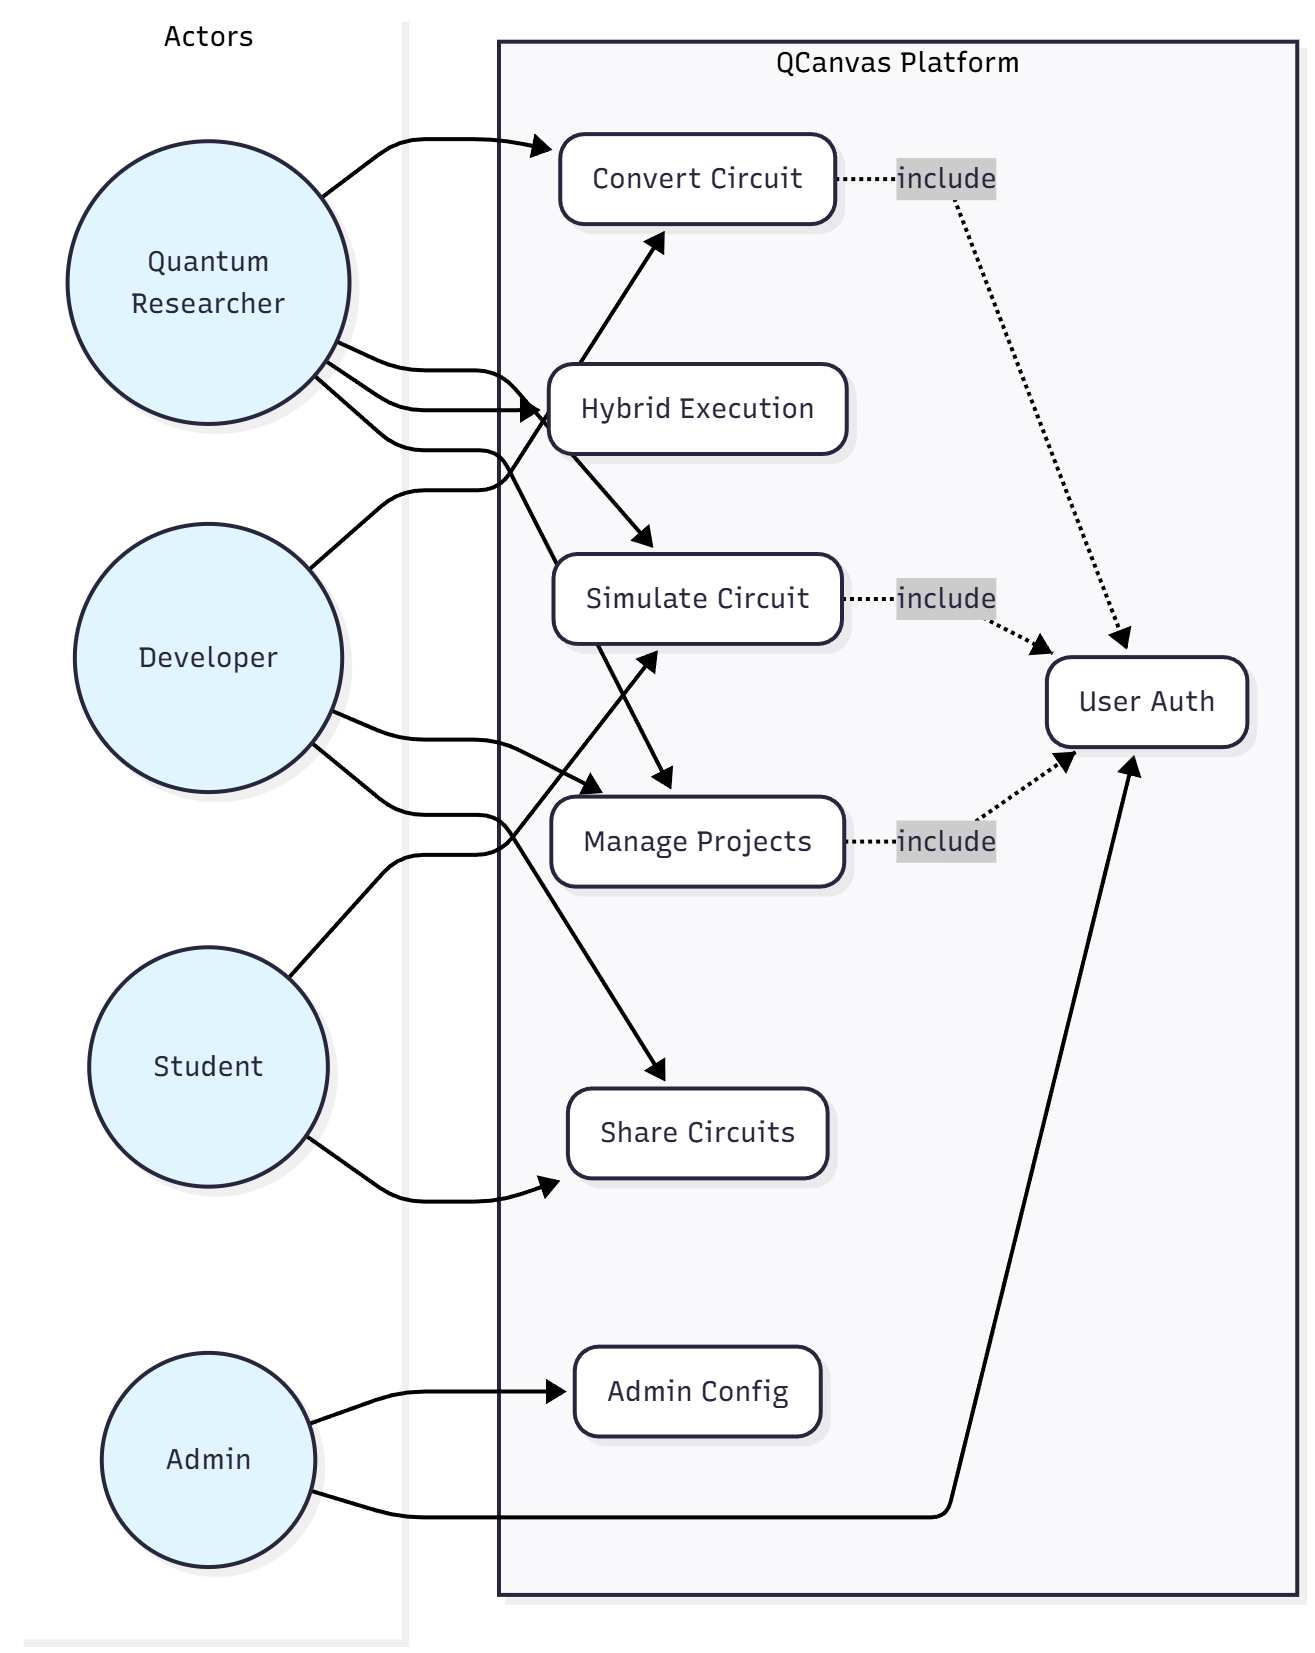
\includegraphics[width=\linewidth]{FYP-UseCase.png}
    \caption{Use Case Diagram}
    \label{fig:usecase}
\end{figure}

\clearpage
\section{Domain Model Diagram}
This diagram shows the core entities (Circuit, ConversionRequest, SimulationJob, SimulationResult, User, Project, Achievement, Recipe) and key relationships that support conversion, simulation, and educational features.
\begin{figure}[H]
    \centering
    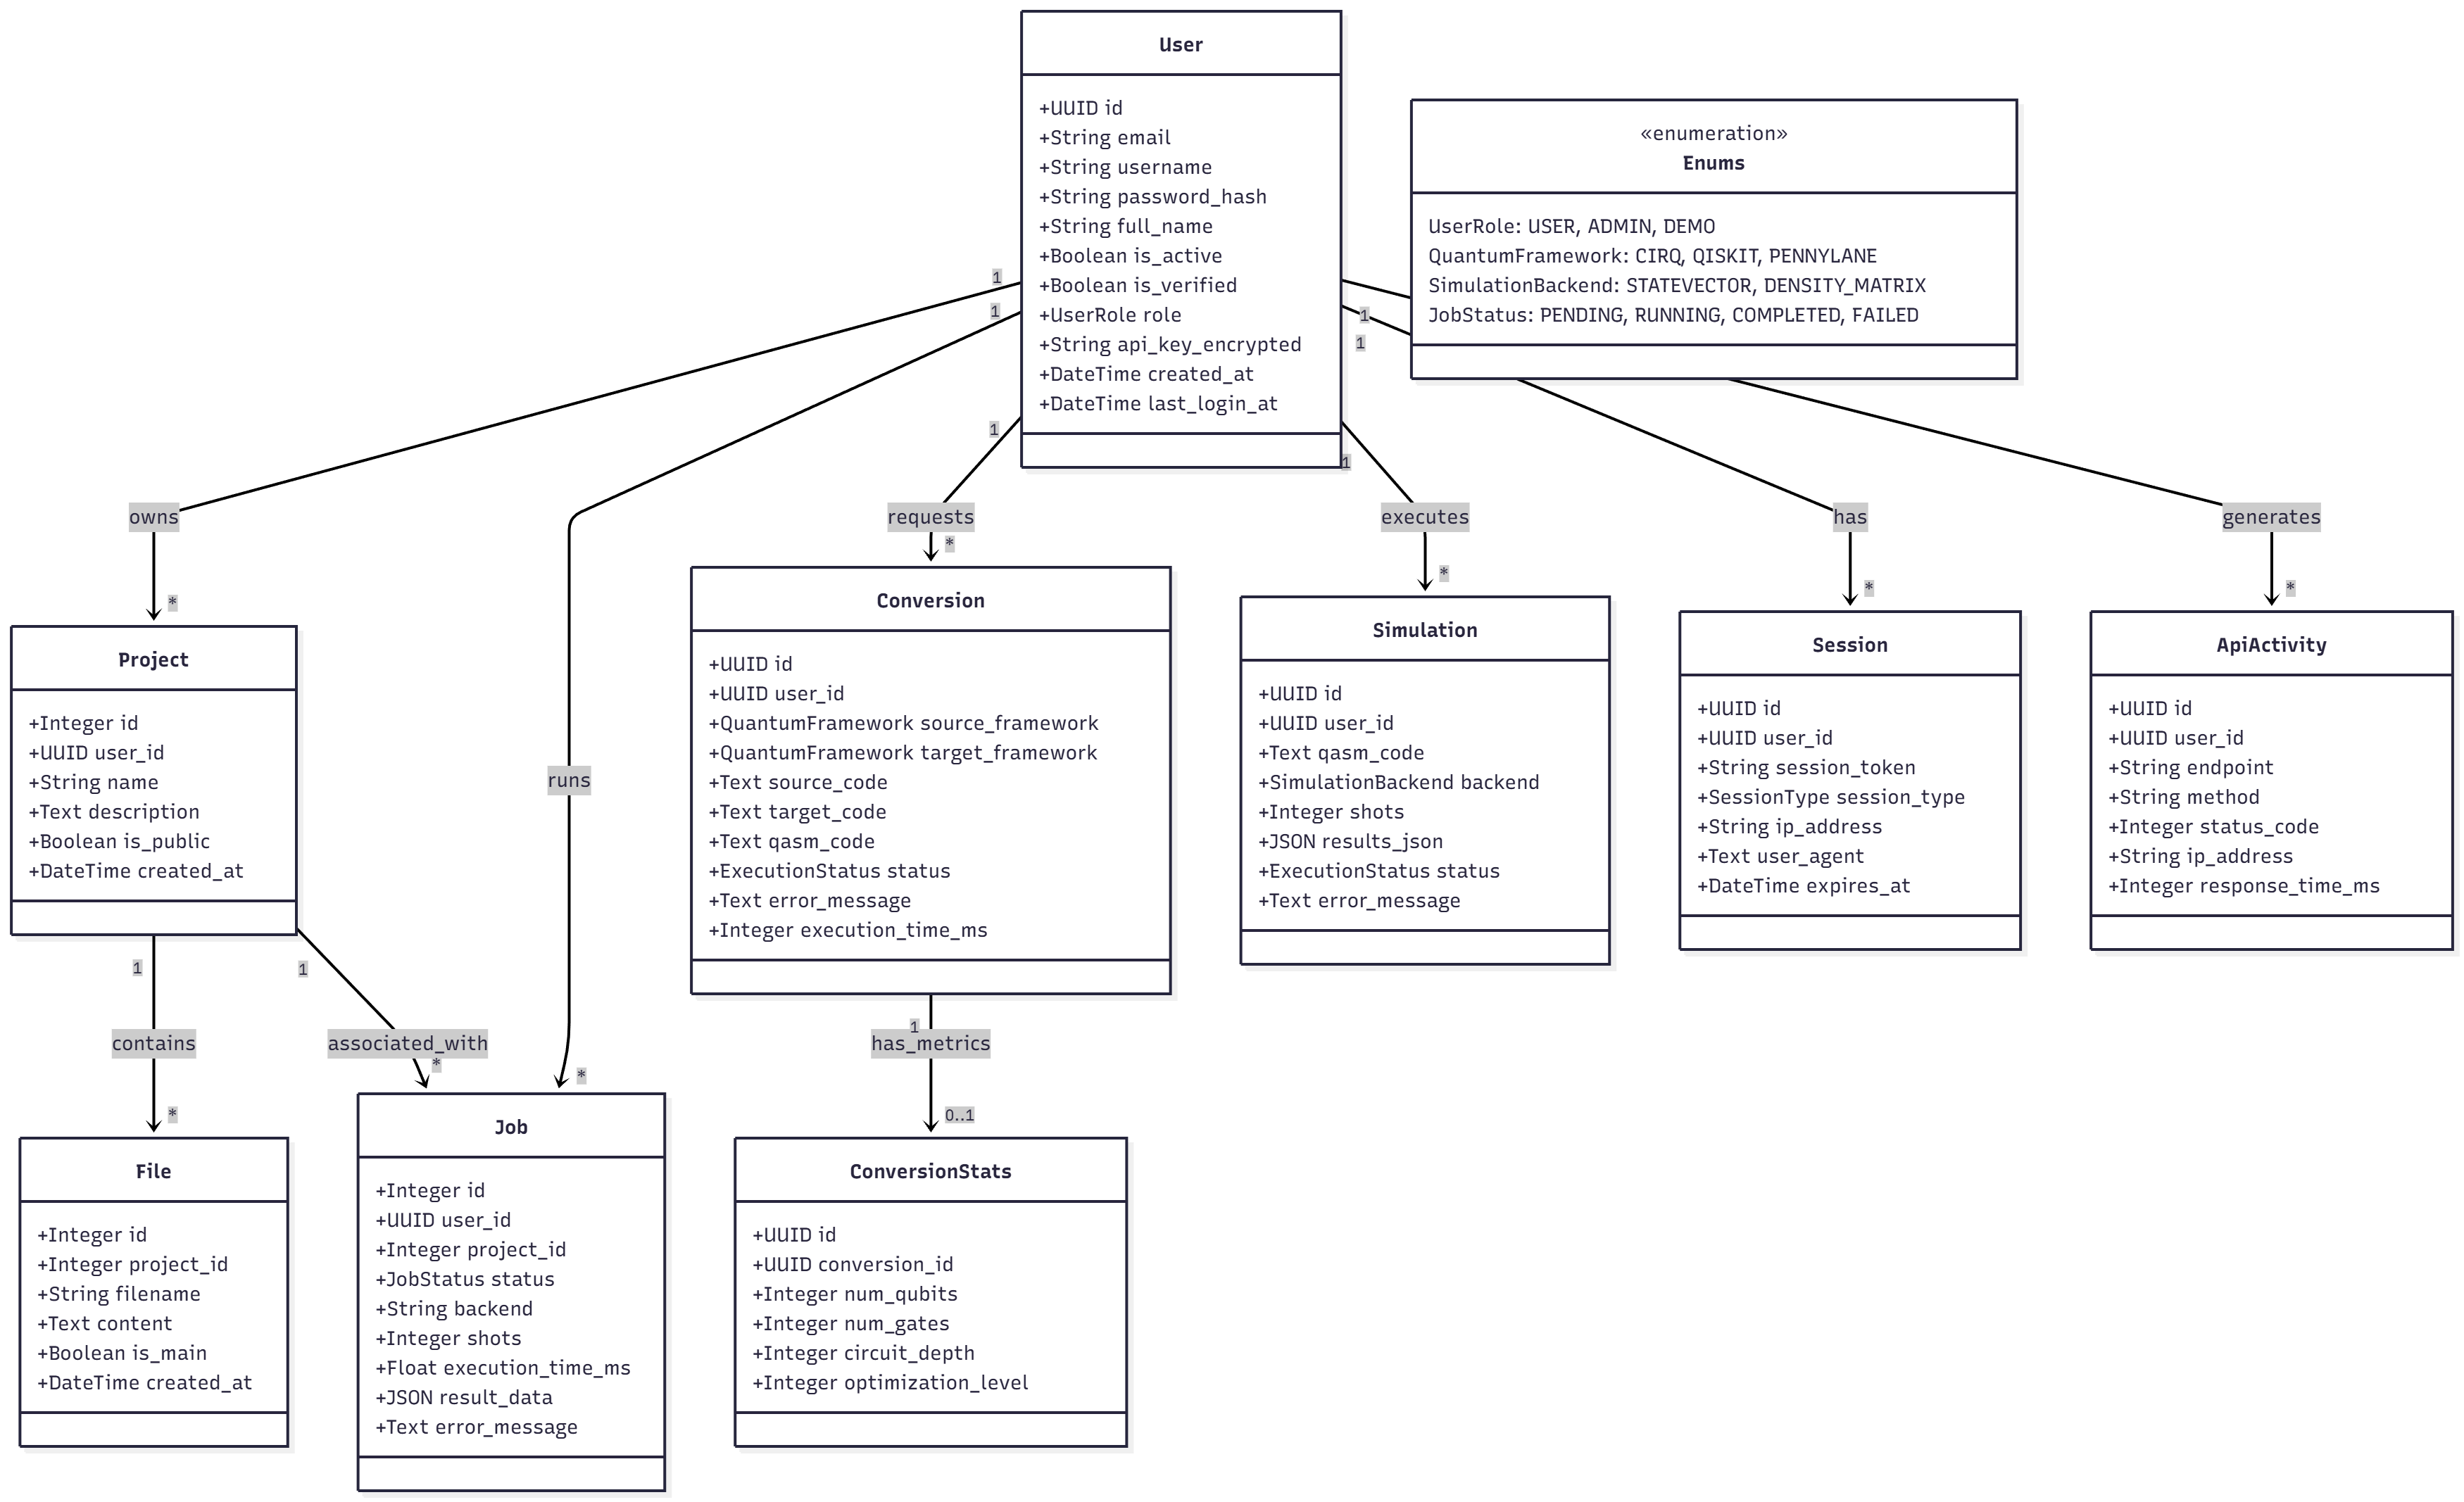
\includegraphics[width=\linewidth]{FYP-DomainModel.png}
    \caption{Domain Model}
    \label{fig:domain-model}
\end{figure}

\chapter{System Overview}
\label{ch:system-overview}

The system architecture of QCanvas follows a modular layered design separating conversion, validation, simulation, and UI concerns. This design ensures scalability, maintainability, and flexibility while supporting the hybrid CPU--QPU execution model \cite{peruzzo2014variational}. The QSim SDK operates as an independently deployable execution kernel that is integrated into the QCanvas backend while also being accessible directly via PyPI.

\section{Architectural Design}

QCanvas employs a hybrid architecture where the Next.js frontend handles UI and simple operations, while the FastAPI backend manages complex quantum computations. QCanvas orchestrates compilation and validation; QSim executes circuits on simulation backends. Both the \texttt{qcanvas-sdk} and \texttt{qsim-sdk} are published on PyPI, making their capabilities accessible to the broader Python community beyond the Web IDE.

\subsection{Layered Responsibilities}
\begin{itemize}
    \item \textbf{Presentation Layer (Next.js)}: Monaco editor UI, D3.js circuit visualization, Chart.js results dashboards, gamification and community UI, and client-side state management via Zustand.
    \item \textbf{API Layer (FastAPI)}: REST endpoints for conversion/validation/simulation, WebSocket for progress streams, structured error handling, request validation, authentication, and rate limiting.
    \item \textbf{Conversion Layer (QCanvas SDK)}: AST parsing, intelligent gate mapping, OpenQASM 3.0 generation via \texttt{QASM3Builder}, validation, conversion analytics, and logging.
    \item \textbf{Execution Layer (QSim SDK)}: Simulation backends (statevector, density matrix, stabilizer), job scheduling, result aggregation, caching, and metrics. Independently installable via \texttt{pip install qsim-sdk}.
    \item \textbf{Persistence Layer}: PostgreSQL for user accounts, projects, and conversion history; Redis for caching and session management.
    \item \textbf{Observability Layer}: Health checks, Prometheus metrics, execution time histograms, and structured logging.
\end{itemize}

\subsection{Technology Stack}

\subsubsection{Frontend Technologies}
\begin{itemize}
    \item Next.js 14 with App Router for server-side rendering and routing.
    \item React 18 with TypeScript for type-safe UI development.
    \item Tailwind CSS for styling with a custom quantum-themed design.
    \item Monaco Editor for code editing with custom syntax highlighting.
    \item D3.js for 2D circuit visualization; \texttt{@react-three/fiber} for 3D rendering.
    \item Zustand for lightweight client-side state management.
    \item Chart.js for measurement histogram visualization.
\end{itemize}

\subsubsection{Backend Technologies}
\begin{itemize}
    \item Python 3.11+ for backend logic and quantum libraries.
    \item FastAPI for high-performance async API framework.
    \item Uvicorn ASGI server for production deployment.
    \item Pydantic for data validation and serialization.
    \item SQLAlchemy ORM with PostgreSQL.
    \item Redis for caching and session management.
    \item Alembic for database migrations.
\end{itemize}

\subsubsection{Quantum Computing Stack}
\begin{itemize}
    \item Cirq 1.0+ for Google quantum framework support \cite{cirq_developers_2023}.
    \item Qiskit 0.44+ for IBM quantum framework support \cite{qiskit}.
    \item PennyLane 0.33+ for Xanadu quantum framework support \cite{bergholm2018pennylane}.
    \item Custom OpenQASM 3.0 generator (\texttt{QASM3Builder}) \cite{cross2021openqasm}.
    \item QSim SDK: Custom simulation backends (statevector, density matrix, stabilizer) \cite{nielsen2010quantum}.
    \item Both SDKs deployed to PyPI for community access.
\end{itemize}

\subsection{Hybrid CPU--QPU Execution Model}

\subsubsection{Orchestration Boundary}
\begin{itemize}
    \item \textbf{CPU Responsibilities}: Circuit construction, parameter preparation, AST parsing, OpenQASM generation, validation, pre/post-processing, and result aggregation.
    \item \textbf{QSim/Simulator Responsibilities}: Gate-level circuit execution, statevector/density matrix evolution, measurement sampling, and state snapshot generation.
\end{itemize}

\subsubsection{Data Flow}
\begin{enumerate}
    \item User writes circuit in source framework (Qiskit/Cirq/PennyLane) in the Monaco editor.
    \item Frontend sends code to FastAPI backend via REST API.
    \item Backend parses code using AST or runtime execution.
    \item QCanvas SDK generates OpenQASM 3.0 intermediate representation.
    \item Validation layer checks conformance to supported subset.
    \item QSim SDK executes circuit on selected backend (statevector/density/stabilizer).
    \item Results aggregated and returned via REST/WebSocket.
    \item Frontend visualizes results (histograms, circuit diagrams, statistics).
\end{enumerate}

\section{Design Models}

\subsection{Activity Diagrams}

\subsubsection{Activity Diagram: Circuit Conversion and Execution}
This diagram presents the end-to-end flow from code input in the Monaco editor, through FastAPI conversion and validation services, into QSim execution and results visualization.
\begin{figure}[H]
    \centering
    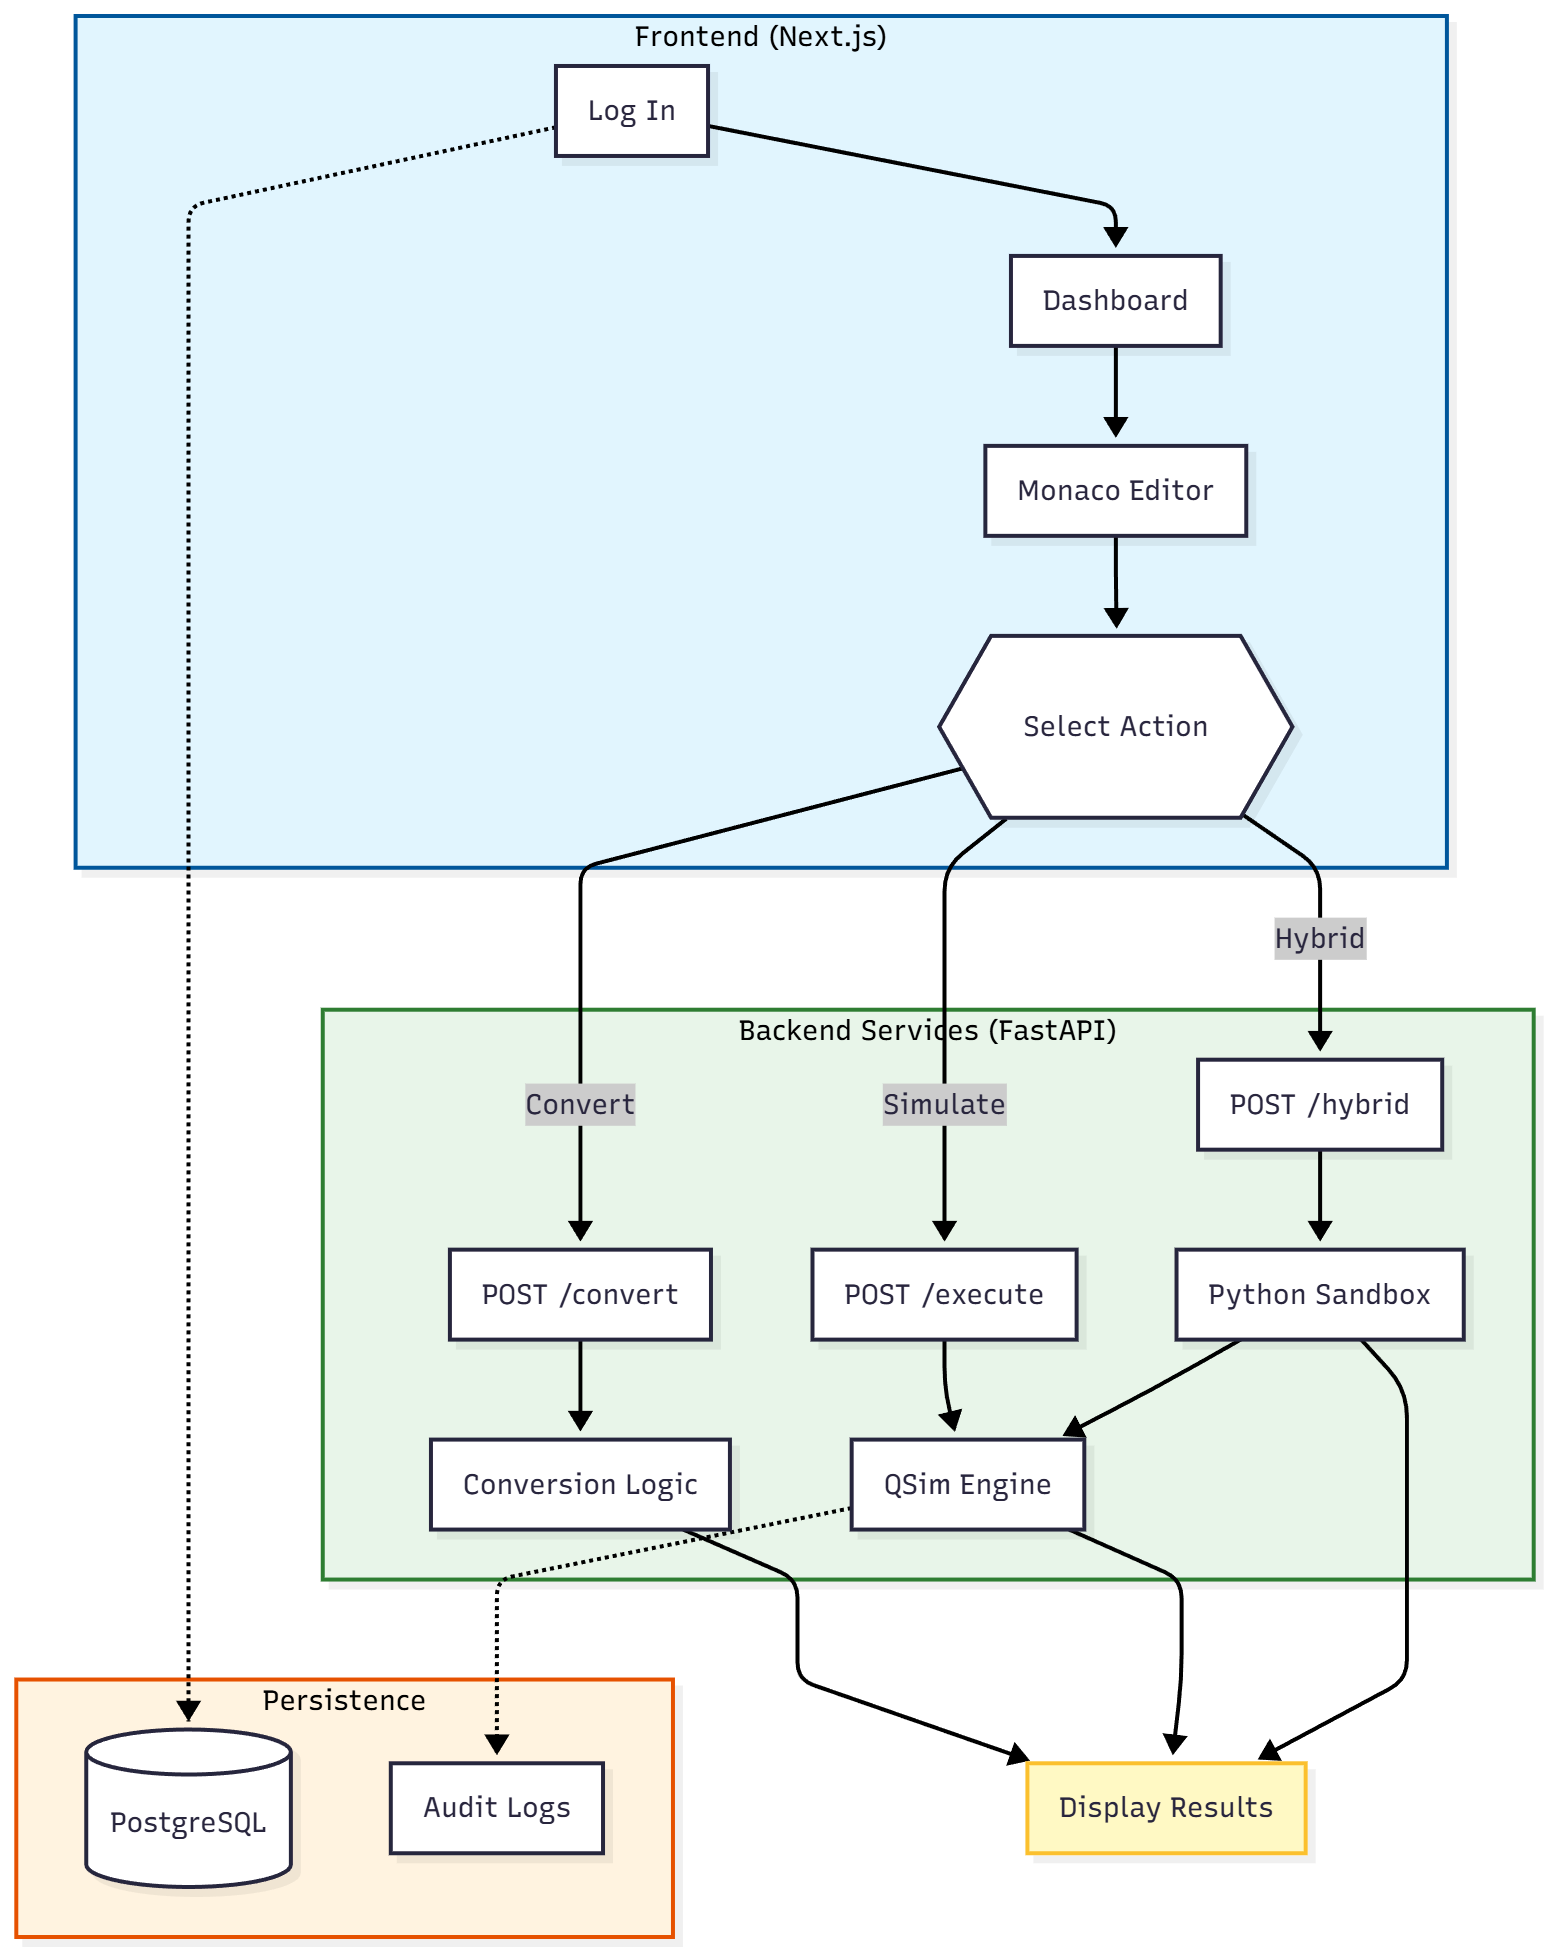
\includegraphics[width=0.65\linewidth]{FYP-Activity-2.png}
    \caption{Activity Diagram --- Circuit Conversion and Execution}
    \label{fig:activity_convert_run}
\end{figure}

\subsubsection{Activity Diagram: User Registration}
This diagram captures the user registration and onboarding flow: a new user submits credentials, FastAPI validates and hashes the password, a PostgreSQL record is created, and a JWT session token is issued.
\begin{figure}[H]
    \centering
    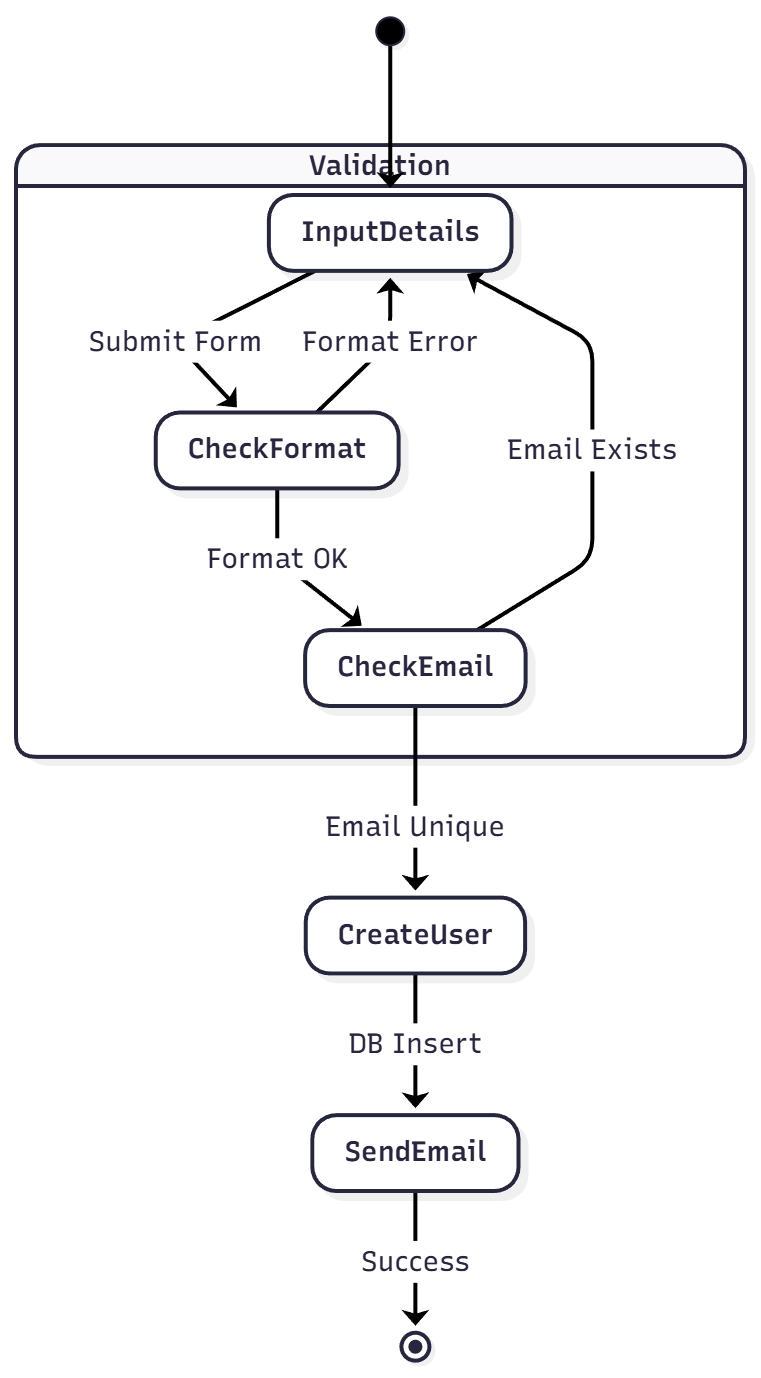
\includegraphics[width=0.55\linewidth]{FYP-ActivityRegistration.png}
    \caption{Activity Diagram --- User Registration}
\end{figure}

\subsection{Sequence Diagrams}

\subsubsection{Sequence Diagram: Unified Execution Flow}
This diagram shows the interaction flow across concrete system components: the user browser, Next.js app, FastAPI routes, ConversionService/SimulationService layer, and the QSim backends.
\begin{figure}[H]
    \centering
    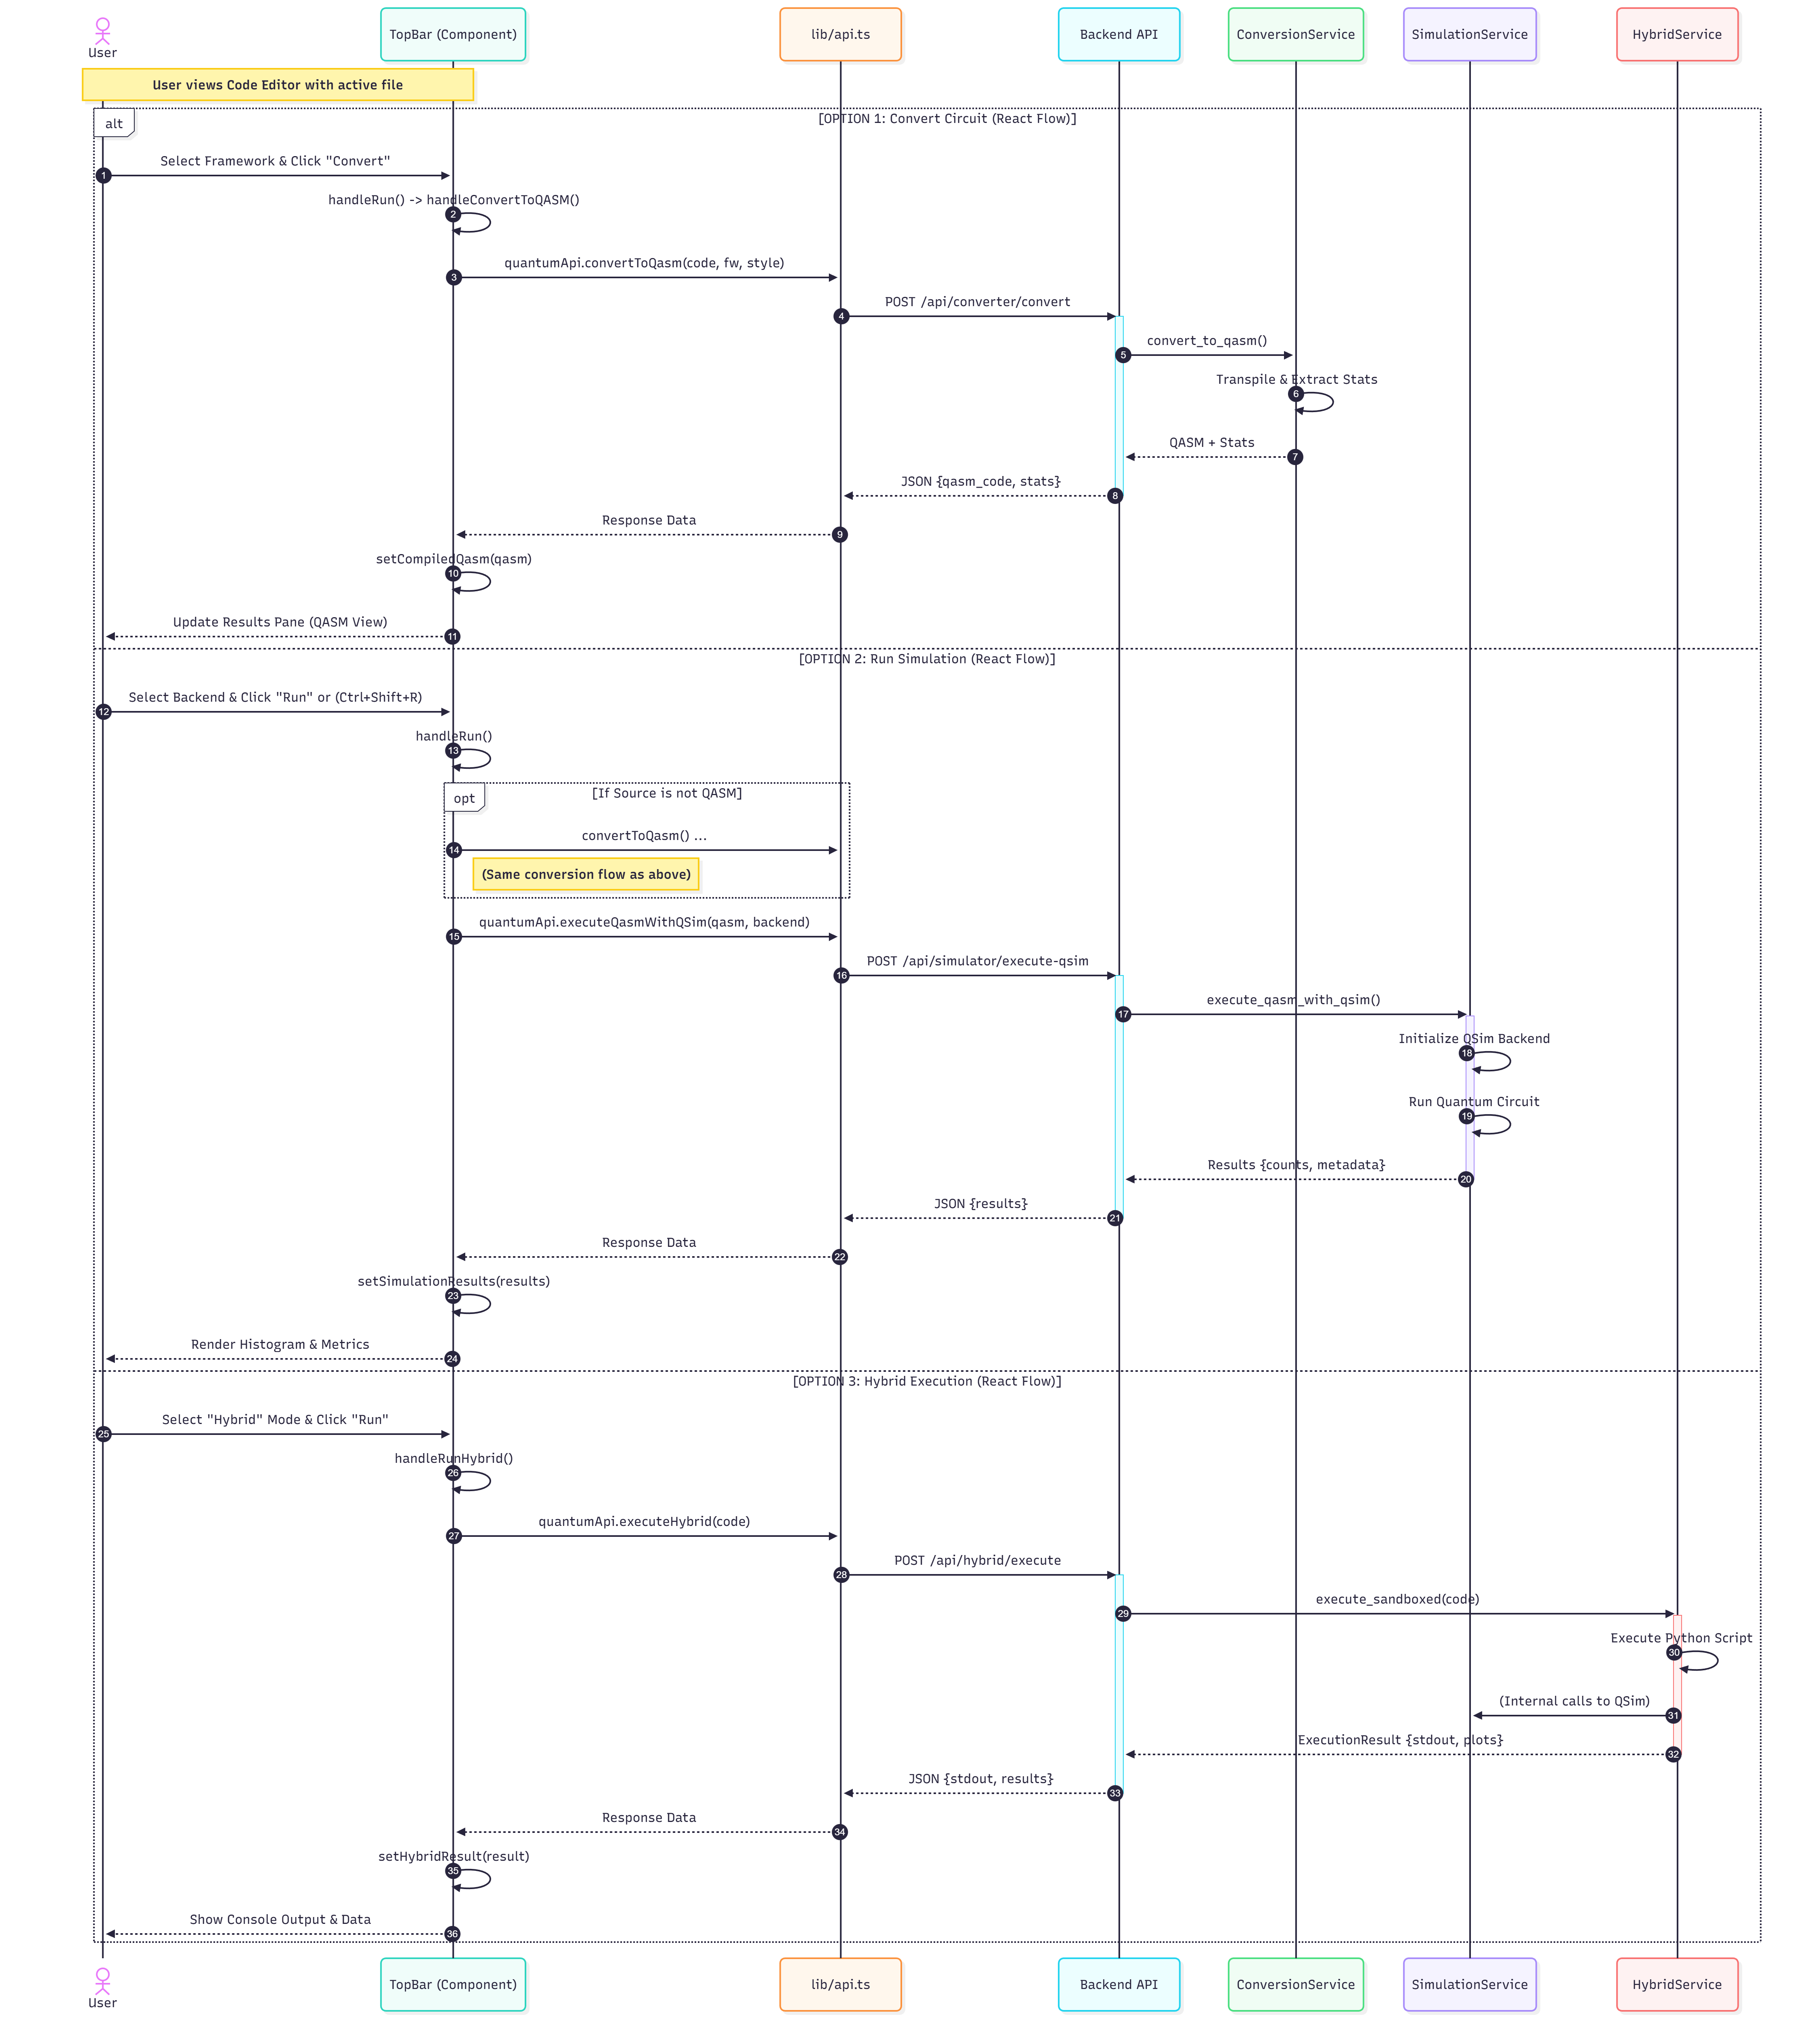
\includegraphics[width=\linewidth]{FYP-SequenceUnified.png}
    \caption{Sequence Diagram --- Unified Flow}
    \label{fig:seq_unified}
\end{figure}

\subsubsection{Sequence Diagram: Authentication}
\begin{figure}[H]
    \centering
    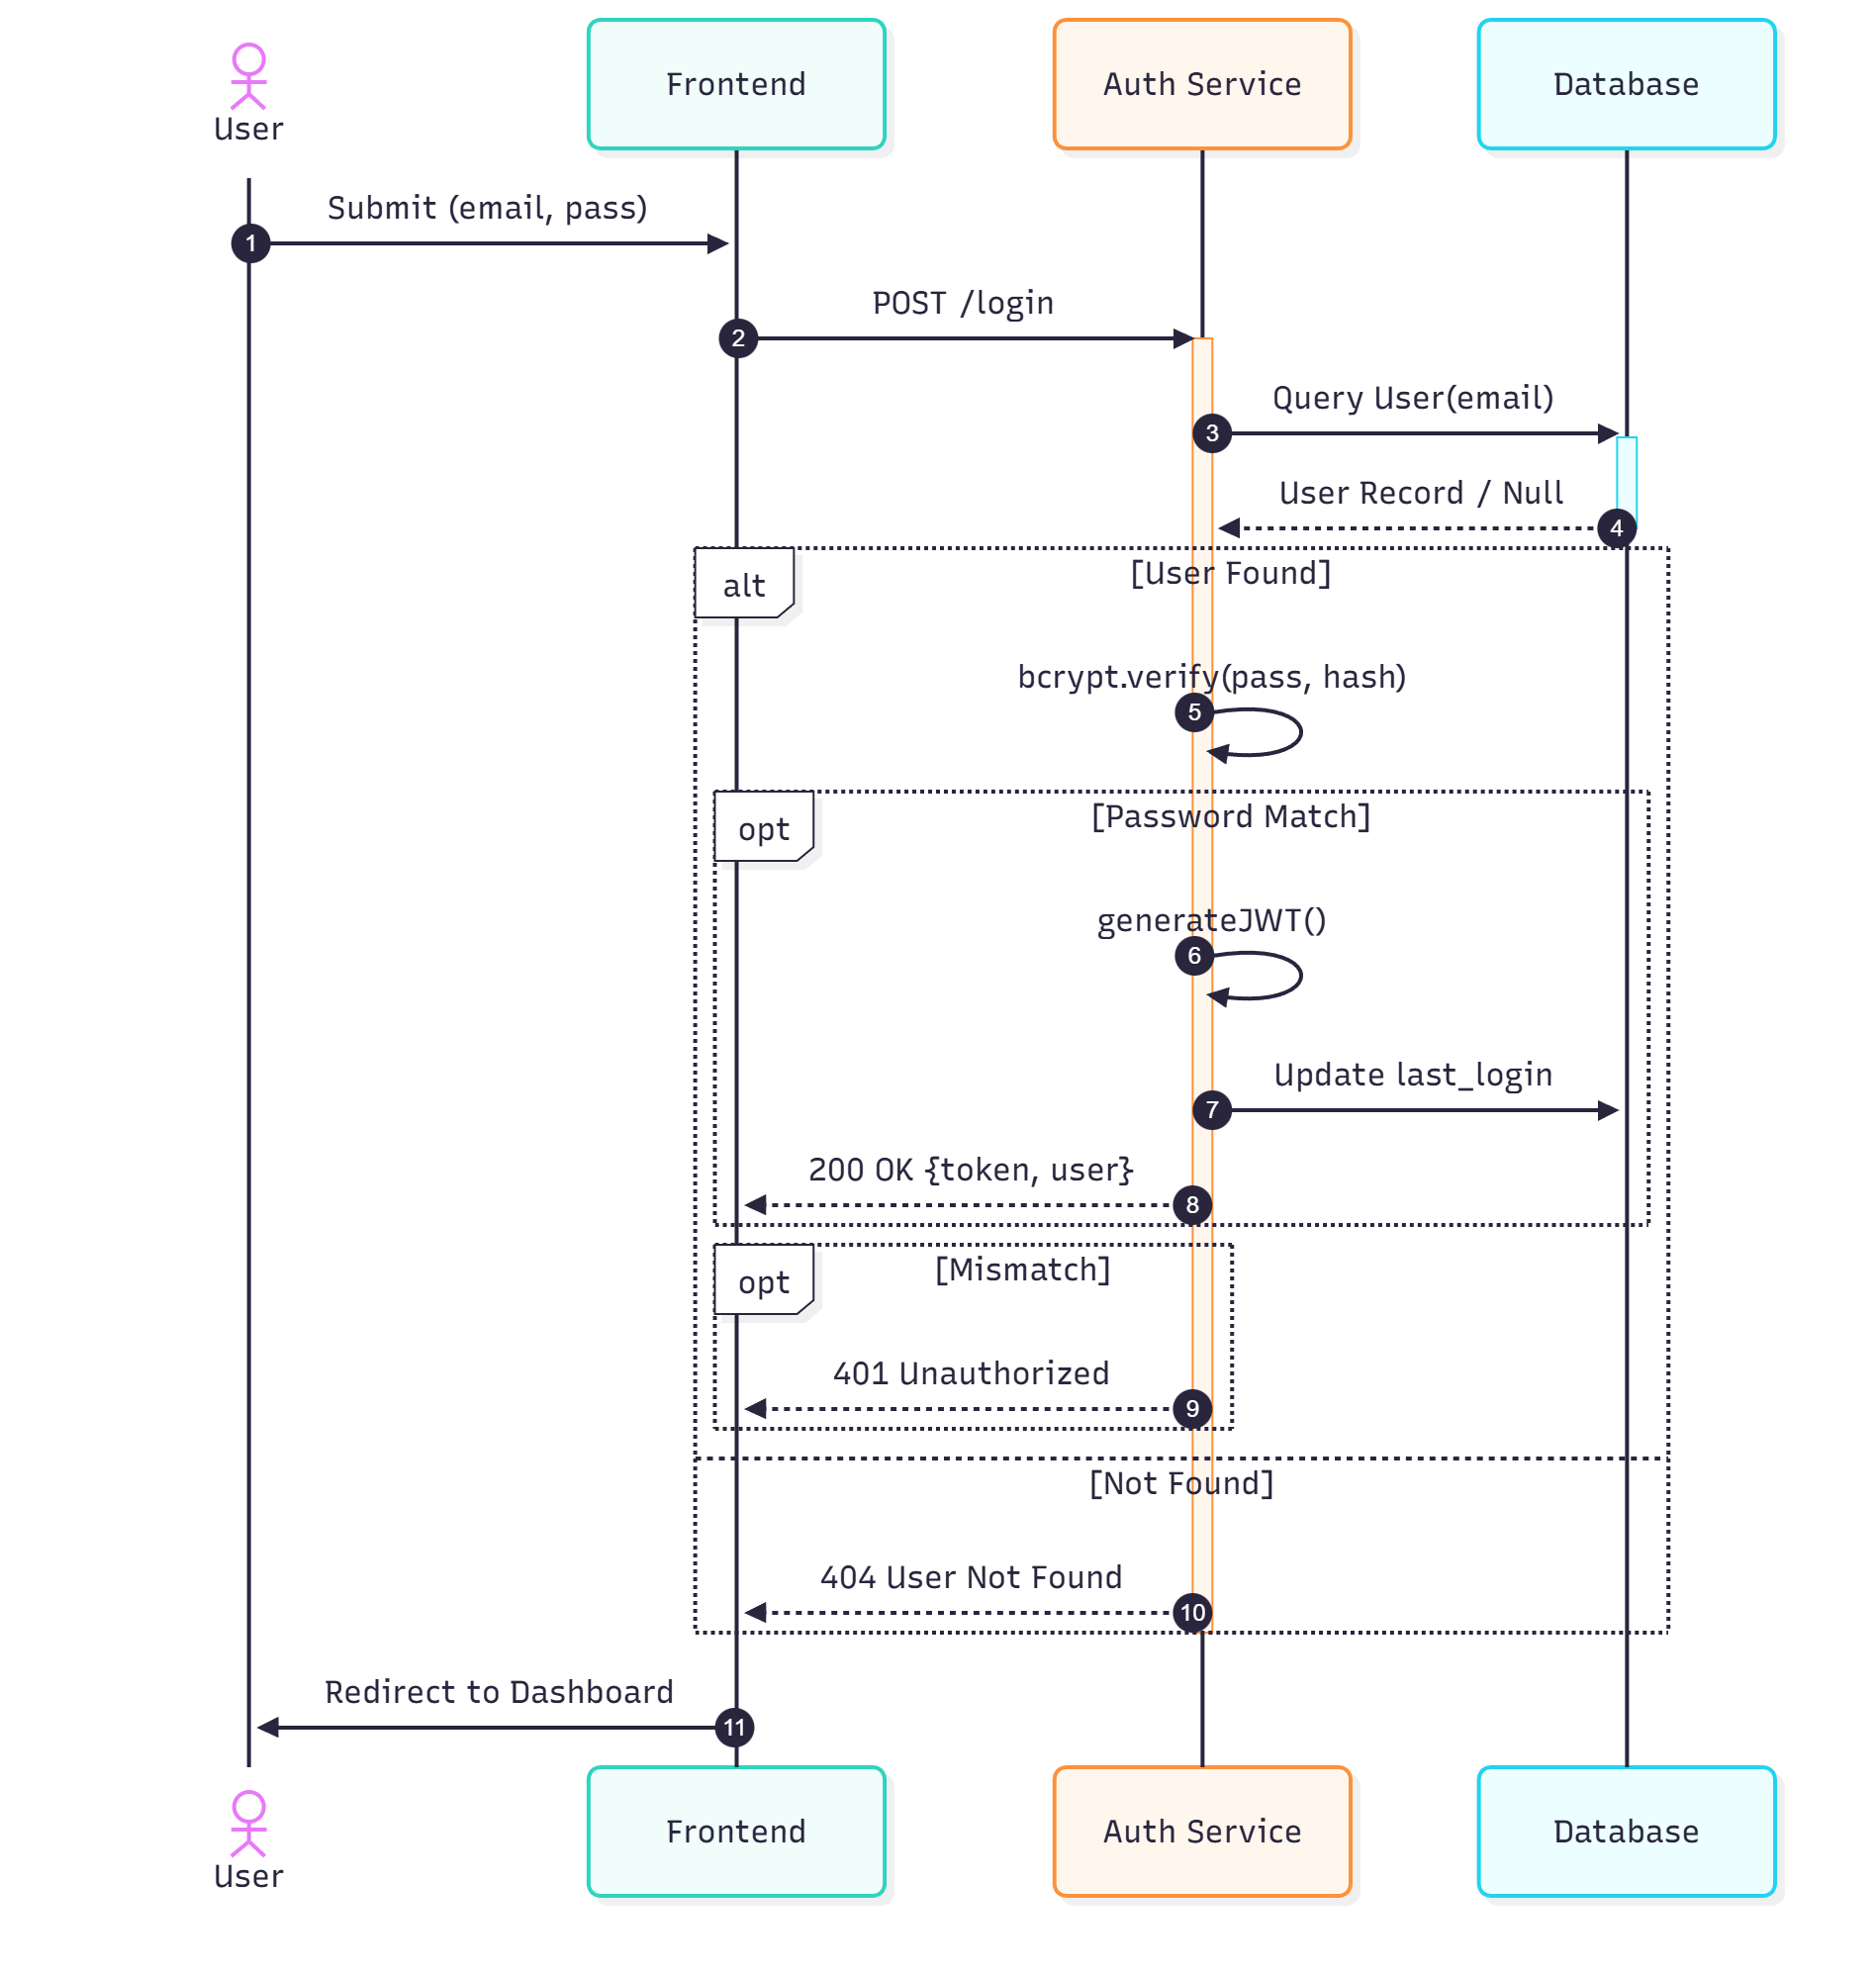
\includegraphics[width=0.95\linewidth]{FYP-SequenceAuth.png}
    \caption{Sequence Diagram --- Authentication}
\end{figure}

\subsubsection{System Sequence Diagrams (SSD)}

\textbf{SSD: Authentication}
\begin{figure}[H]
    \centering
    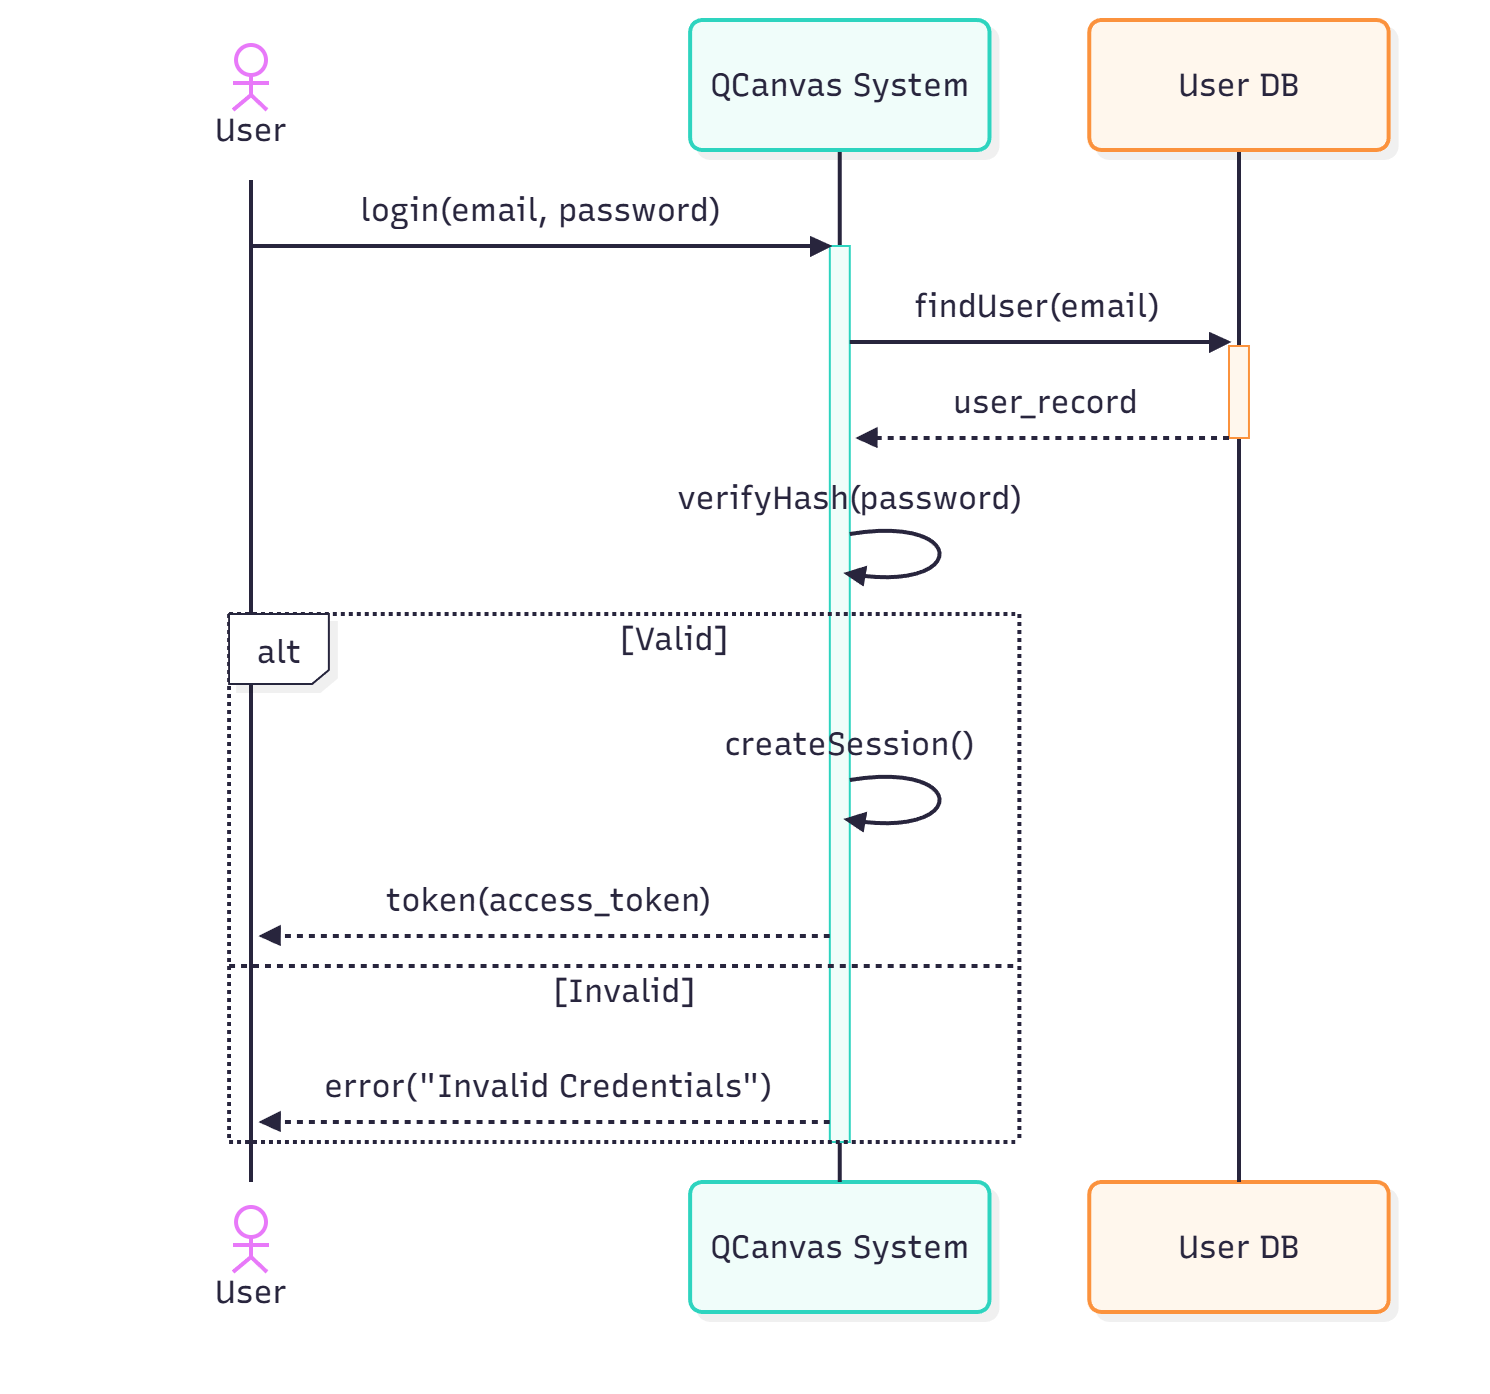
\includegraphics[width=0.95\linewidth]{FYP-Ssd-Auth.png}
    \caption{SSD --- Authentication}
\end{figure}

\textbf{SSD: Conversion}
\begin{figure}[H]
    \centering
    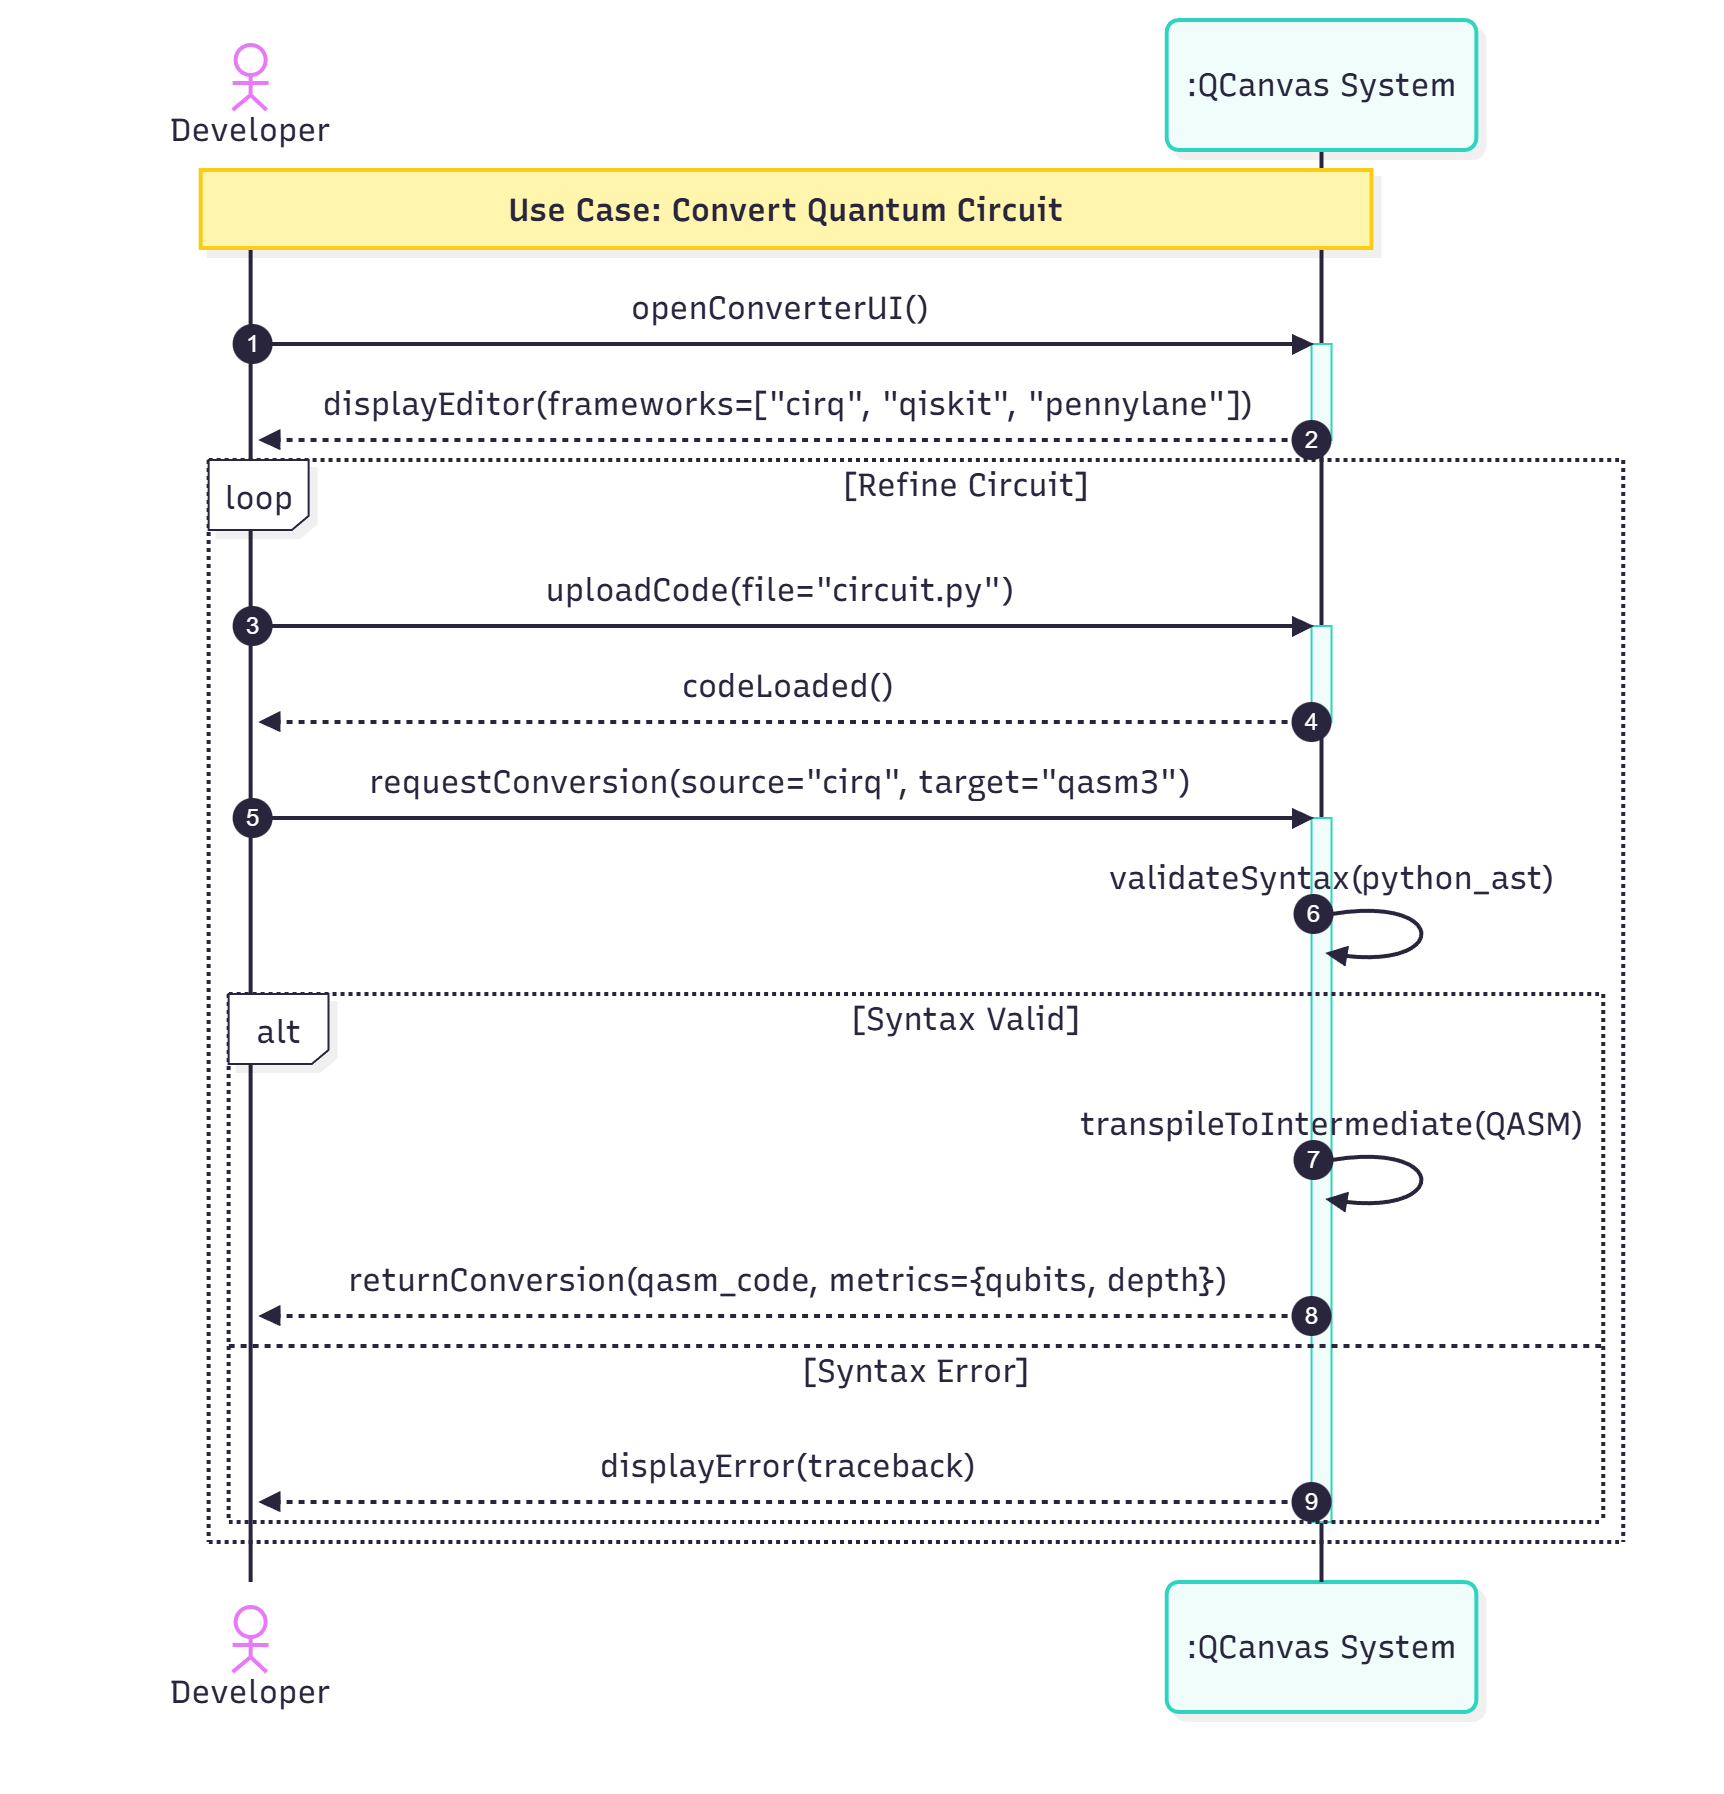
\includegraphics[width=0.92\linewidth]{FYP-Ssd-Conversion.png}
    \caption{SSD --- Conversion}
\end{figure}

\textbf{SSD: Simulation}
\begin{figure}[H]
    \centering
    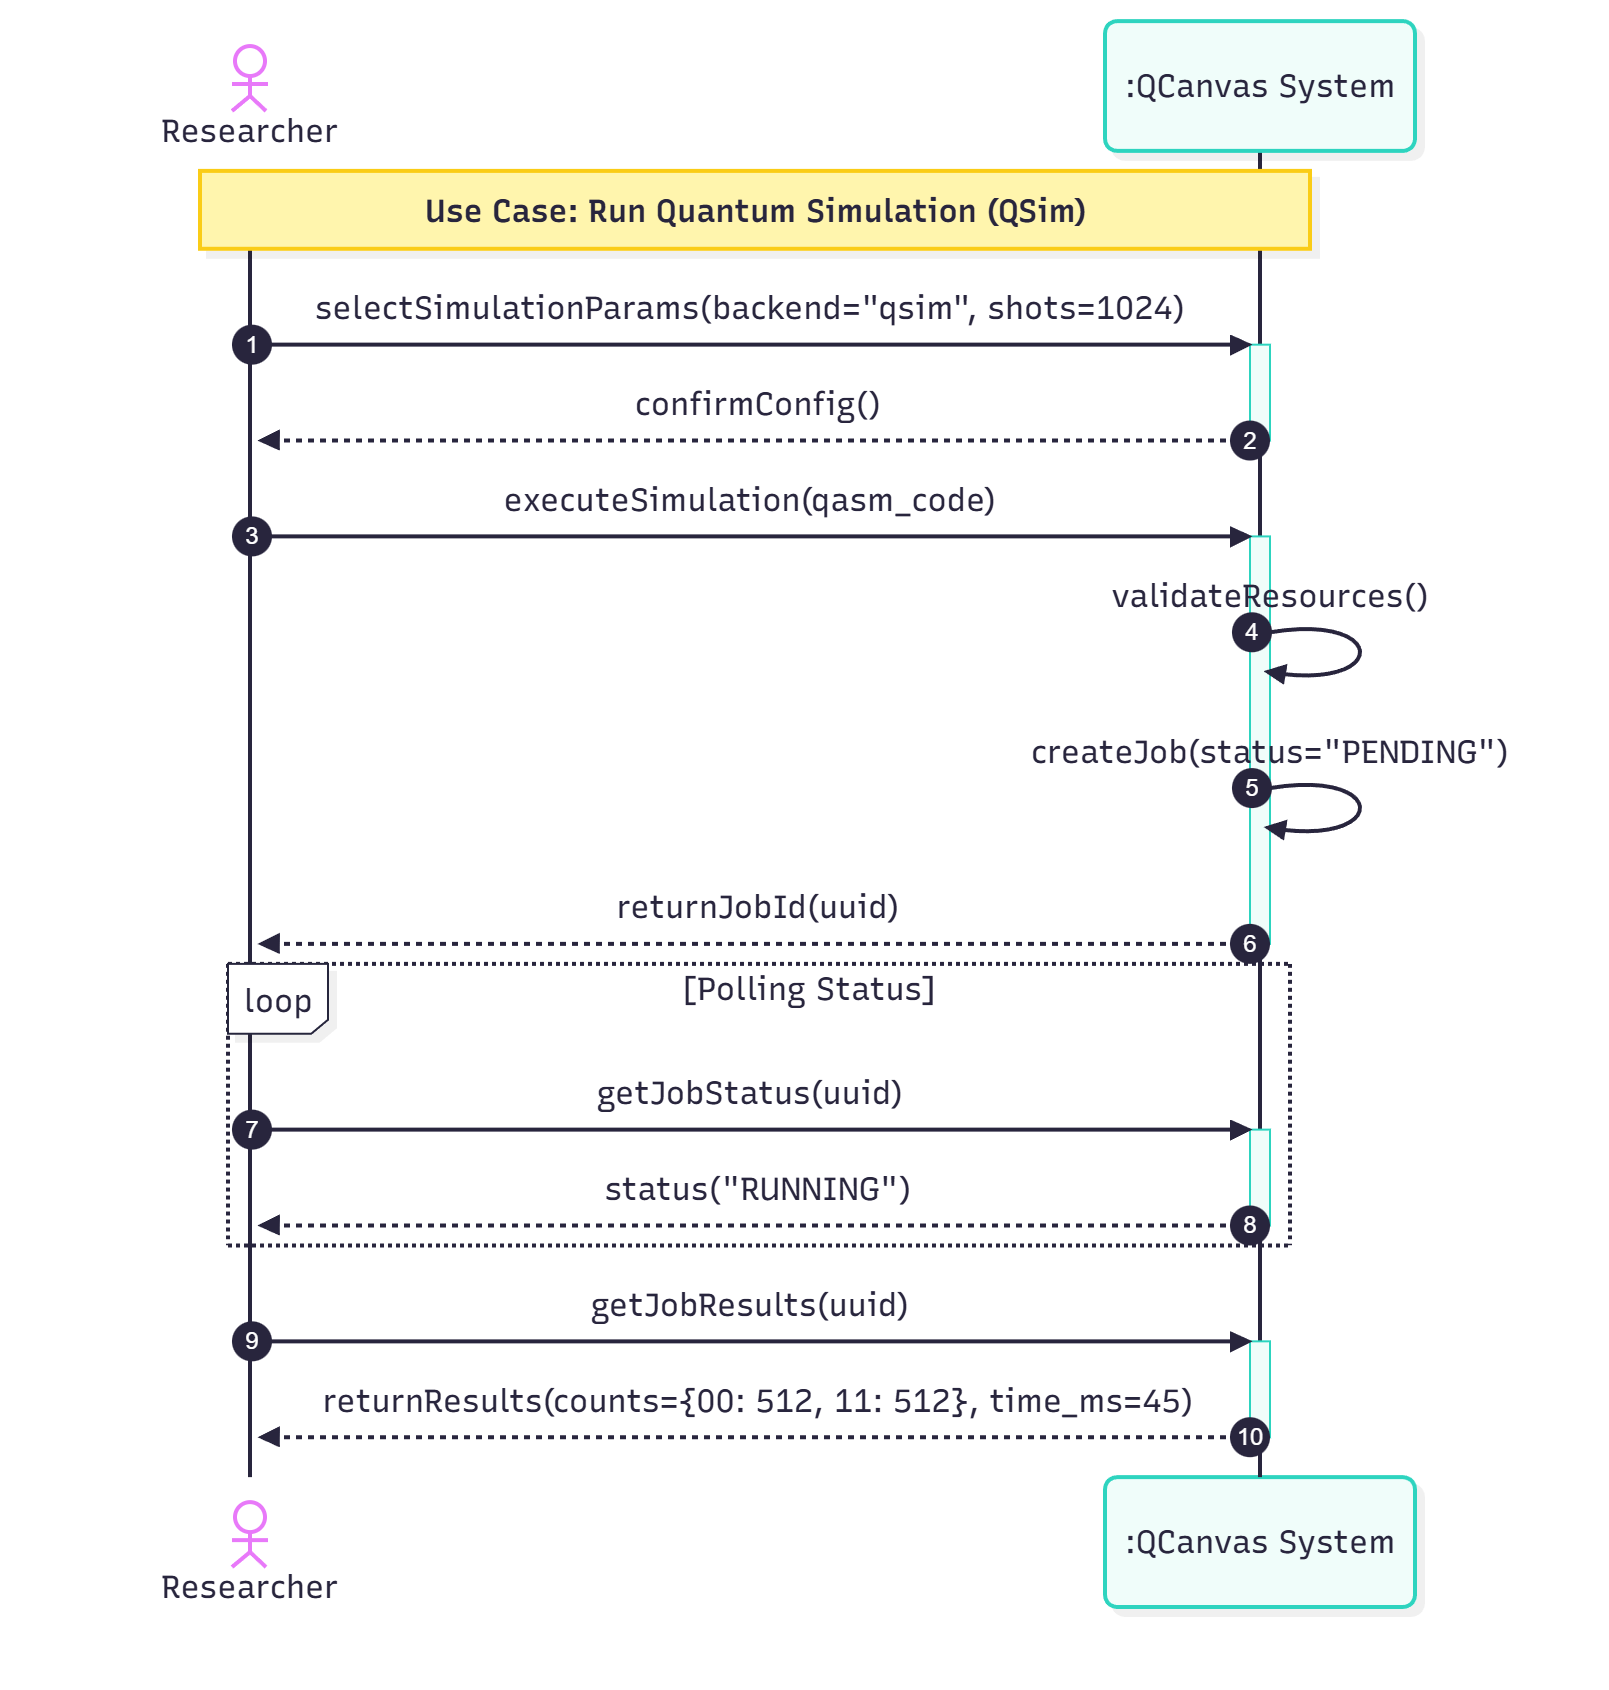
\includegraphics[width=0.95\linewidth]{FYP-Ssd-Simulation.png}
    \caption{SSD --- Simulation}
\end{figure}

\clearpage
\subsection{Architecture Diagram}
This diagram provides a high-level view of the deployed QCanvas stack: the Next.js IDE, FastAPI API layer, \texttt{quantum\_converters} and \texttt{quantum\_simulator} (QSim) packages, PostgreSQL/Redis persistence, and WebSocket/REST communication channels.
\begin{figure}[H]
    \centering
    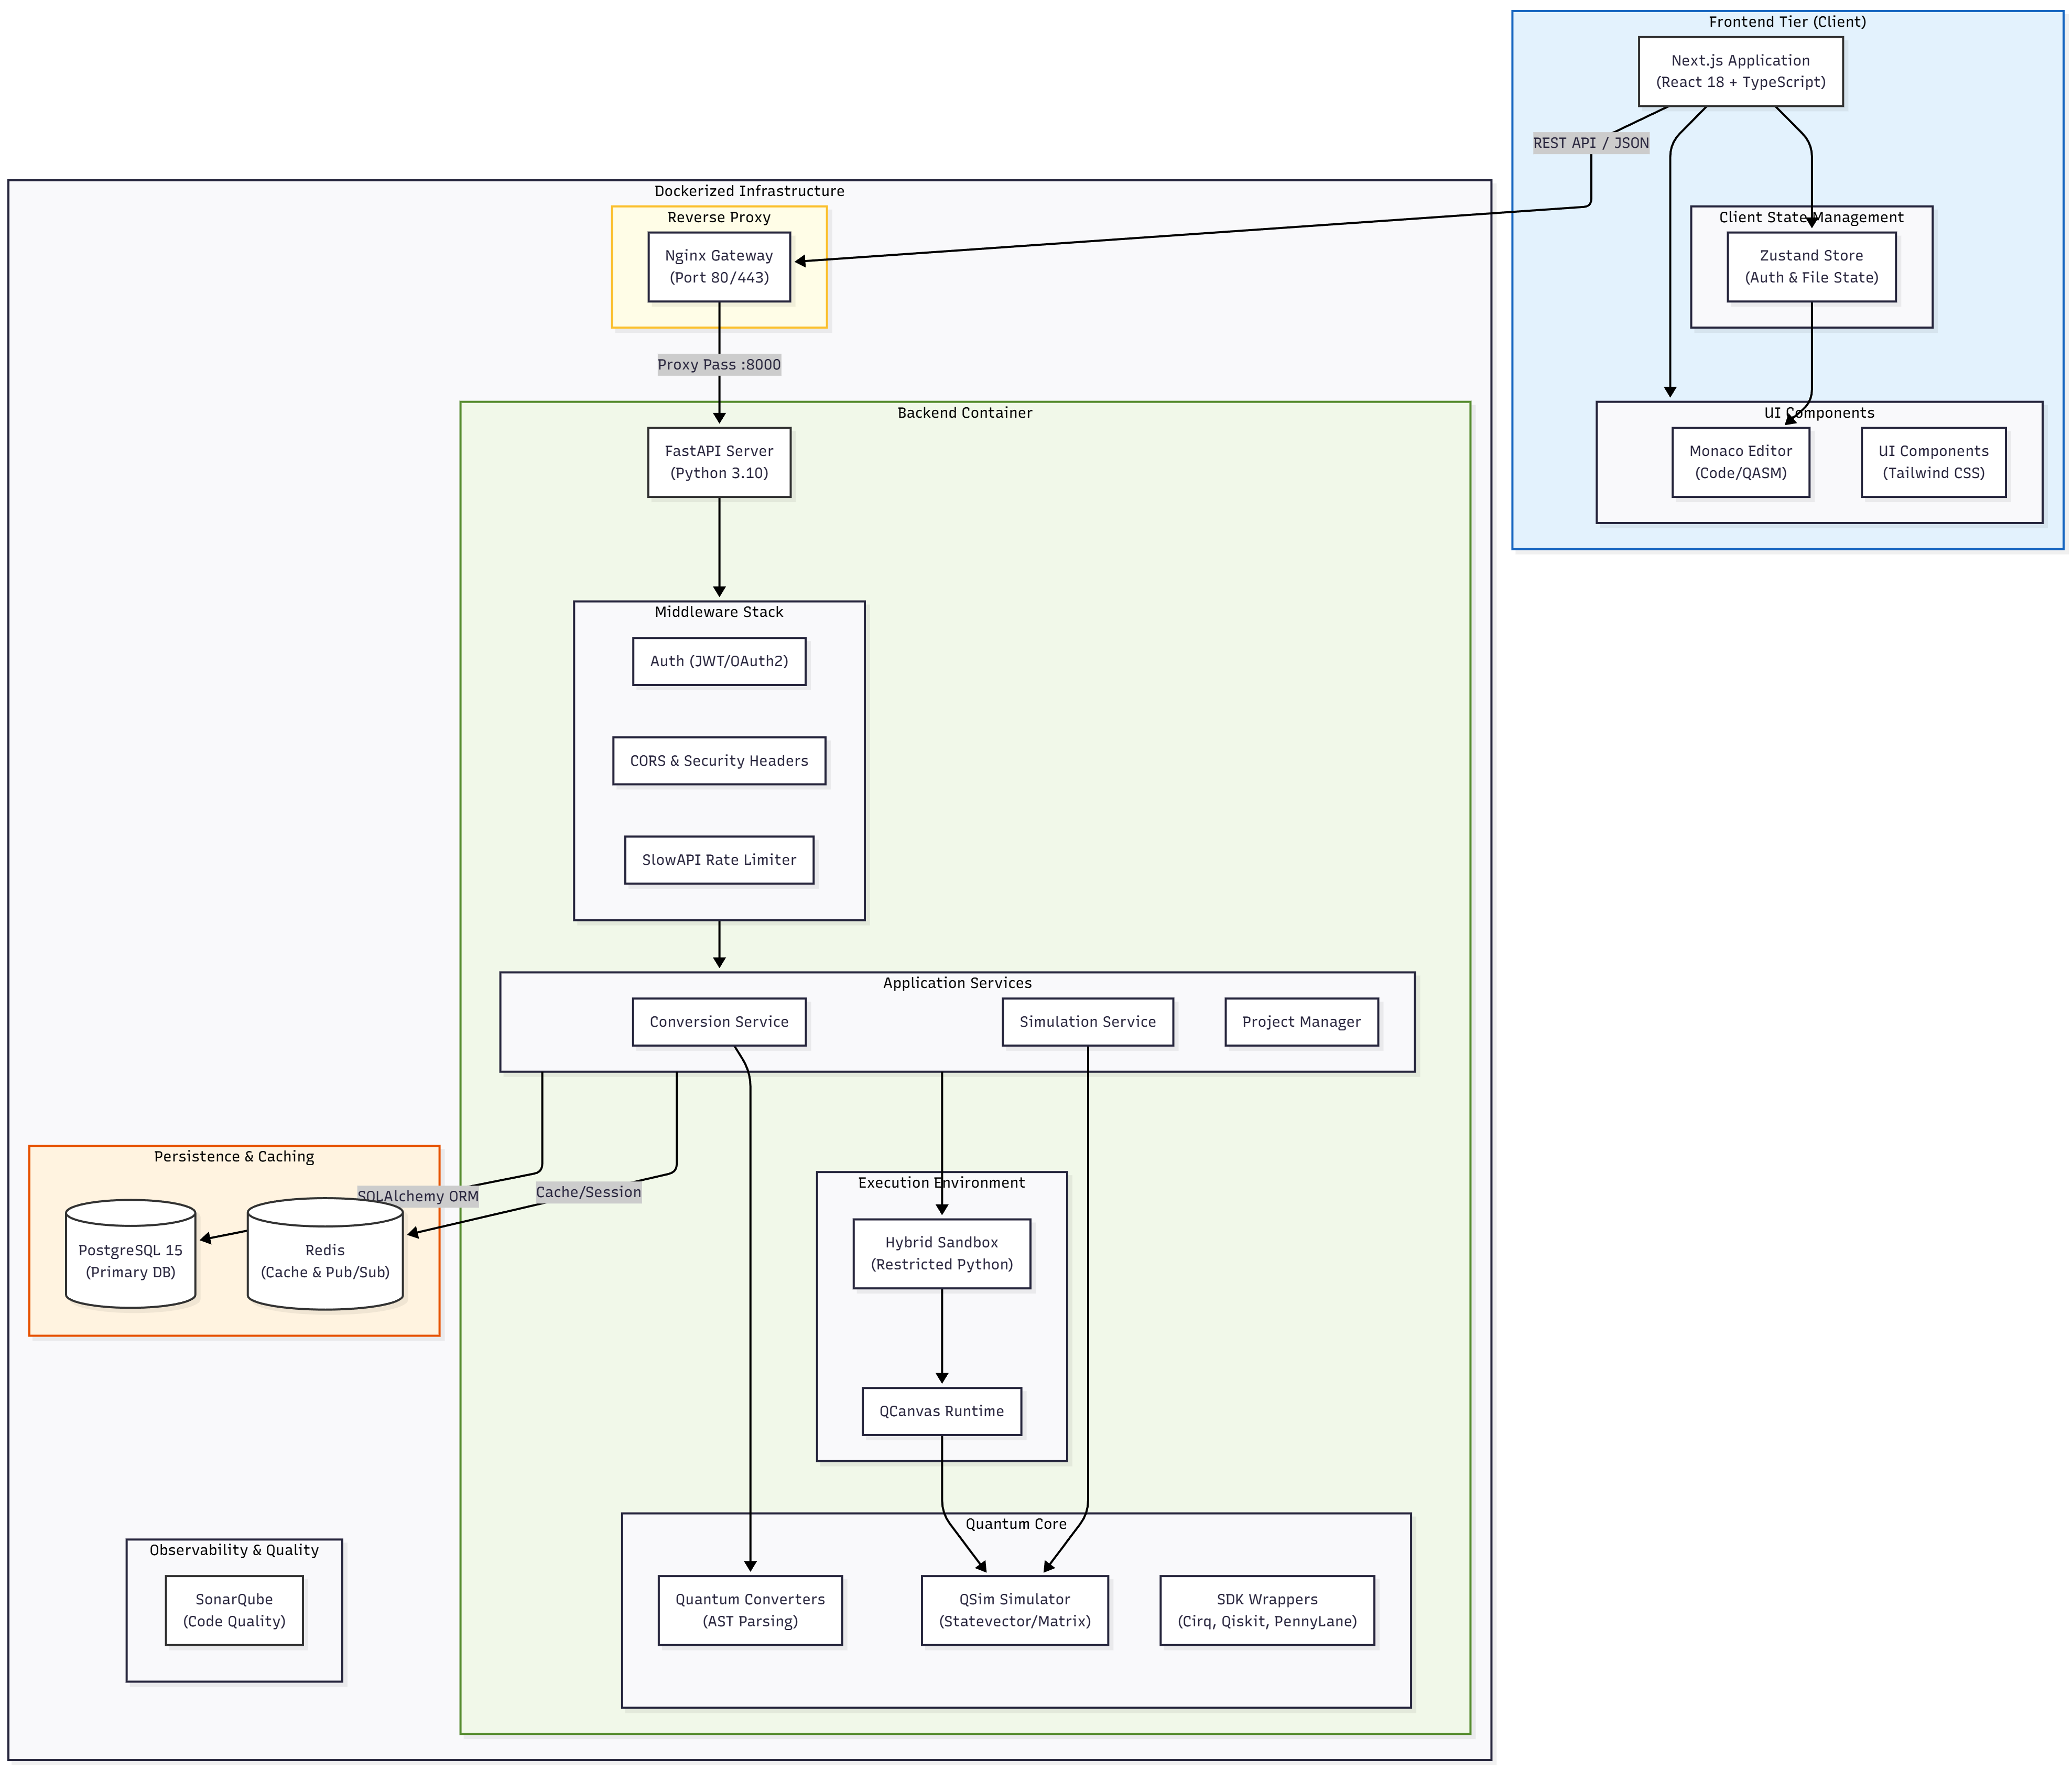
\includegraphics[width=0.95\linewidth]{FYP-SystemArchitecture.png}
    \caption{System Architecture Diagram}
    \label{fig:architecture}
\end{figure}

\clearpage
\subsection{Component Diagram}
This diagram depicts concrete module boundaries: editor and results components in the frontend, API routes and services in the backend, conversion/validation modules, QSim simulation backends, and shared utilities.
\begin{figure}[H]
    \centering
    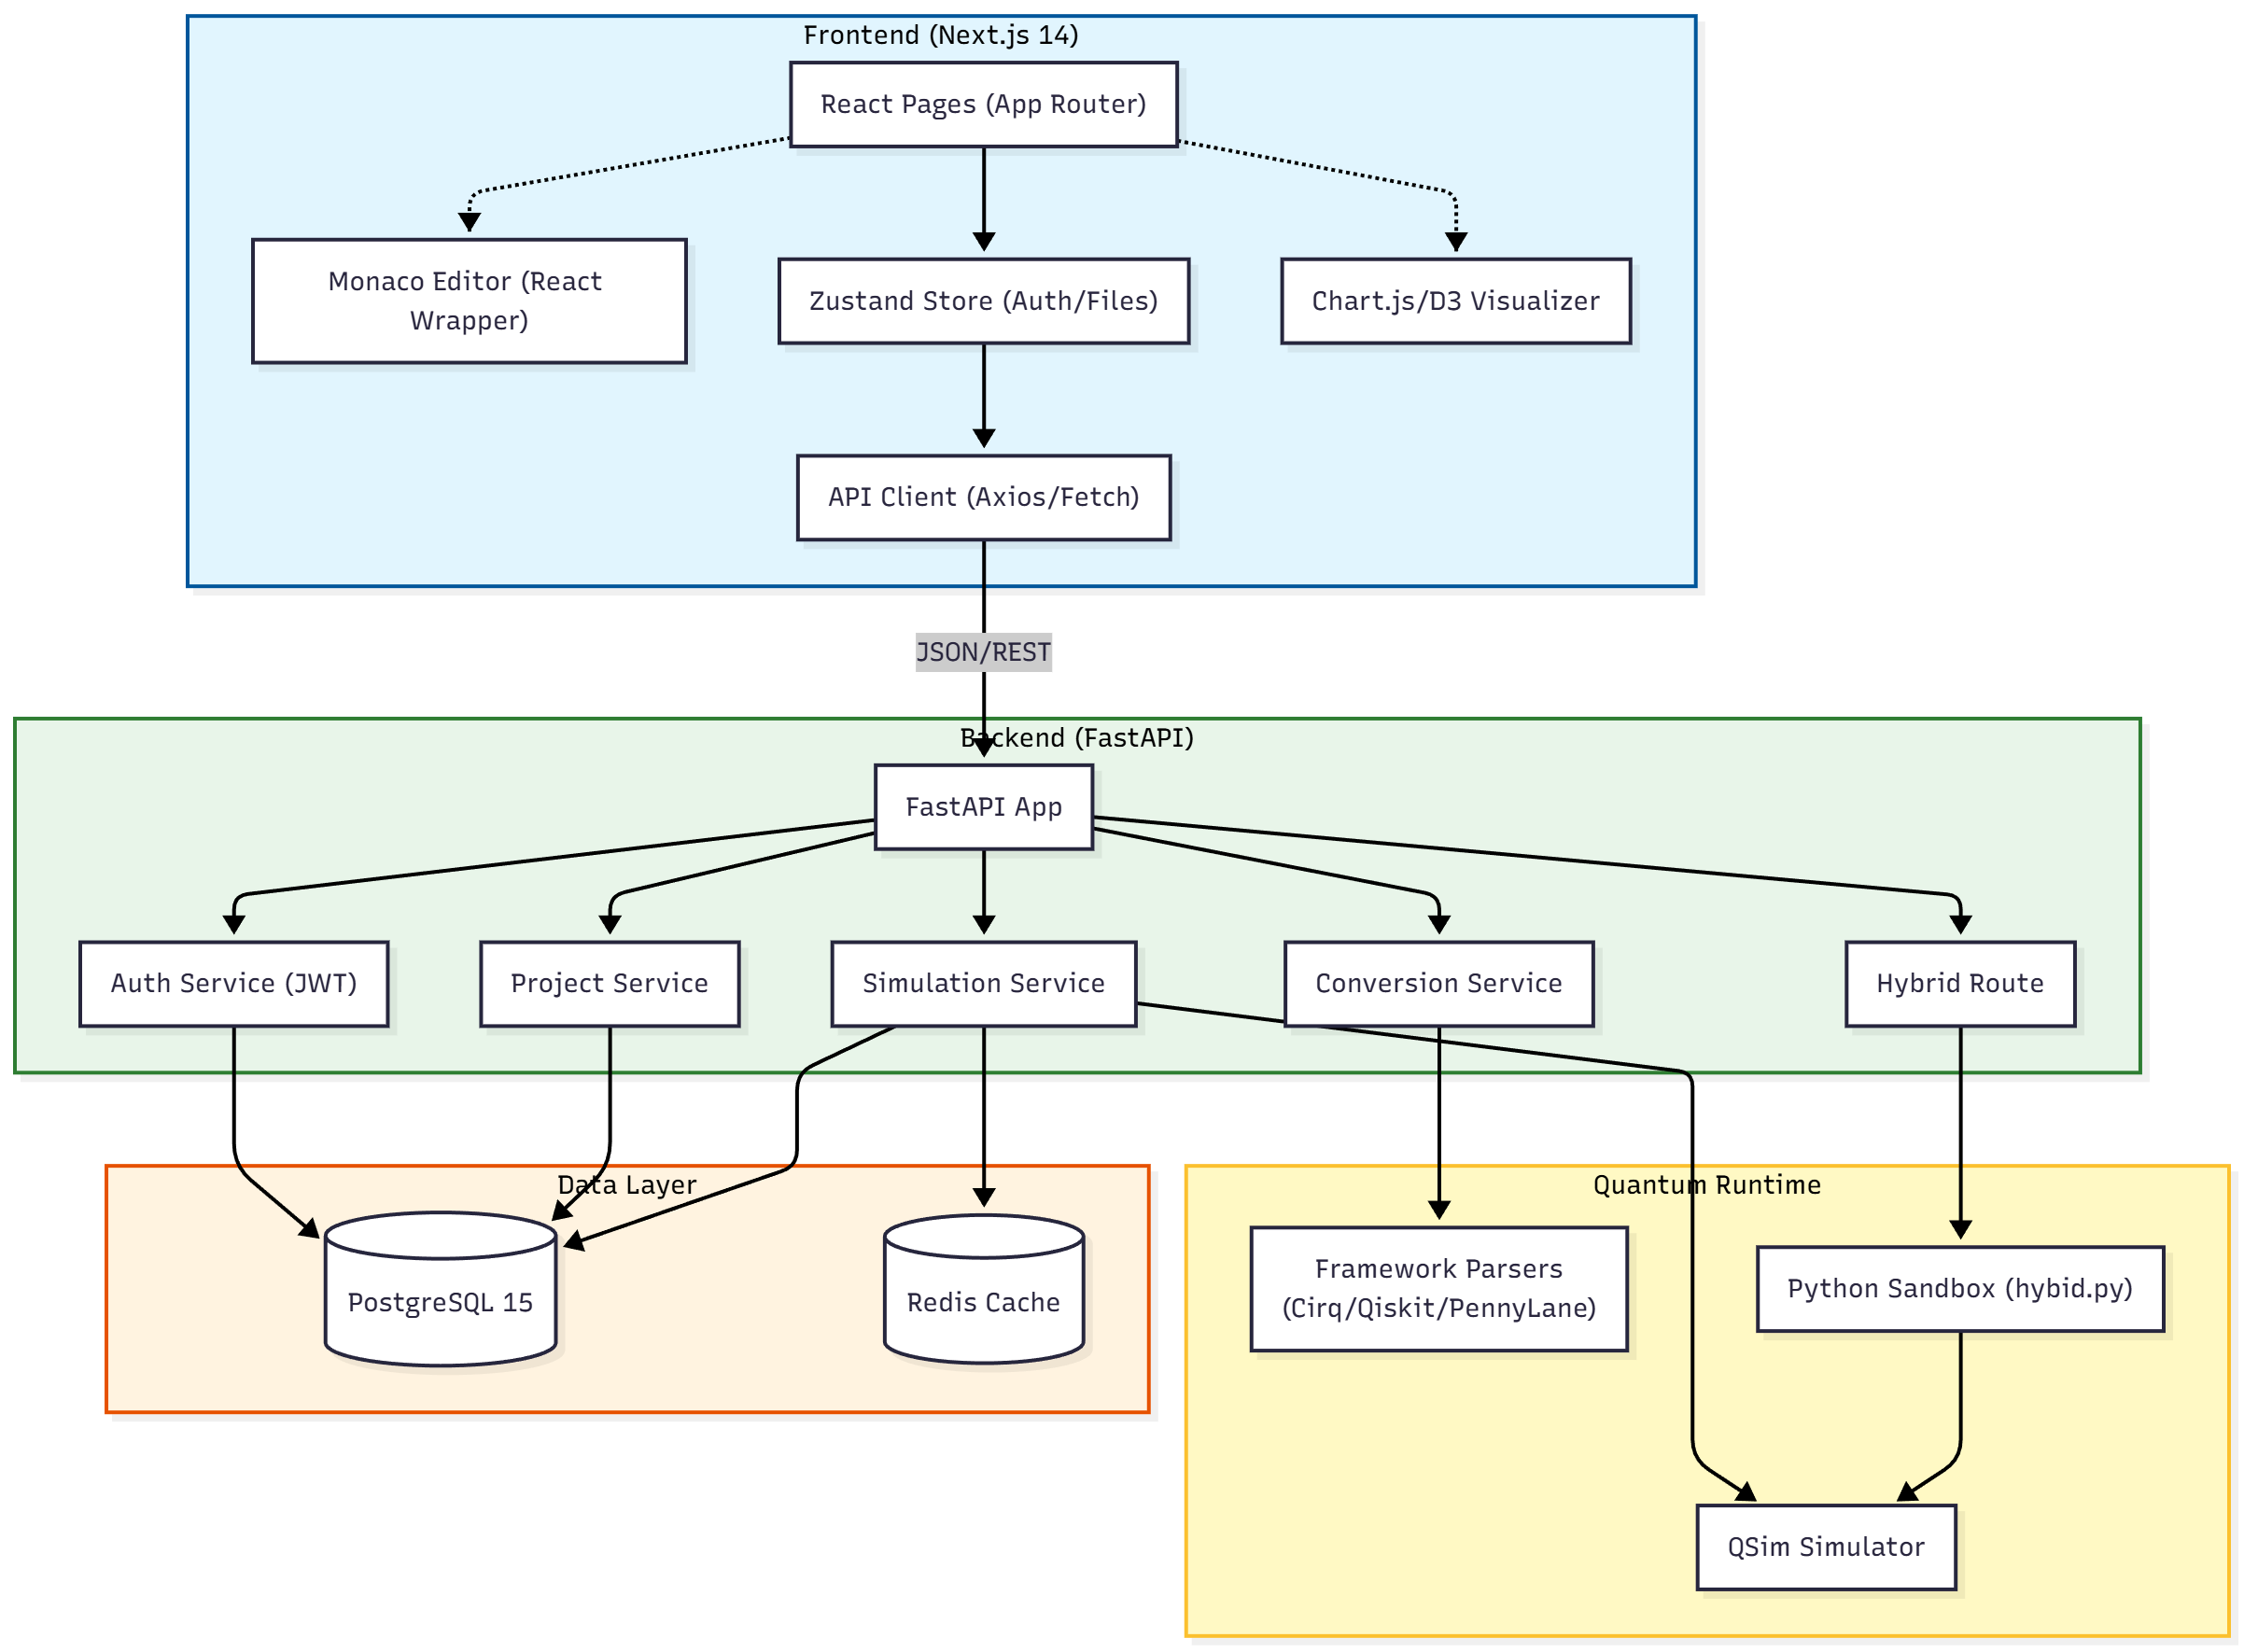
\includegraphics[width=0.95\linewidth]{FYP-Component.png}
    \caption{Component Diagram}
    \label{fig:component}
\end{figure}

\clearpage
\subsection{Package Diagram}
This diagram outlines the actual package organization across the frontend (Next.js \texttt{app}, \texttt{components}, \texttt{lib}), backend (\texttt{app/api}, \texttt{core}, \texttt{services}, \texttt{models}), \texttt{quantum\_converters} (parsers, converters, optimizers), and \texttt{quantum\_simulator} (QSim) libraries.
\begin{figure}[H]
    \centering
    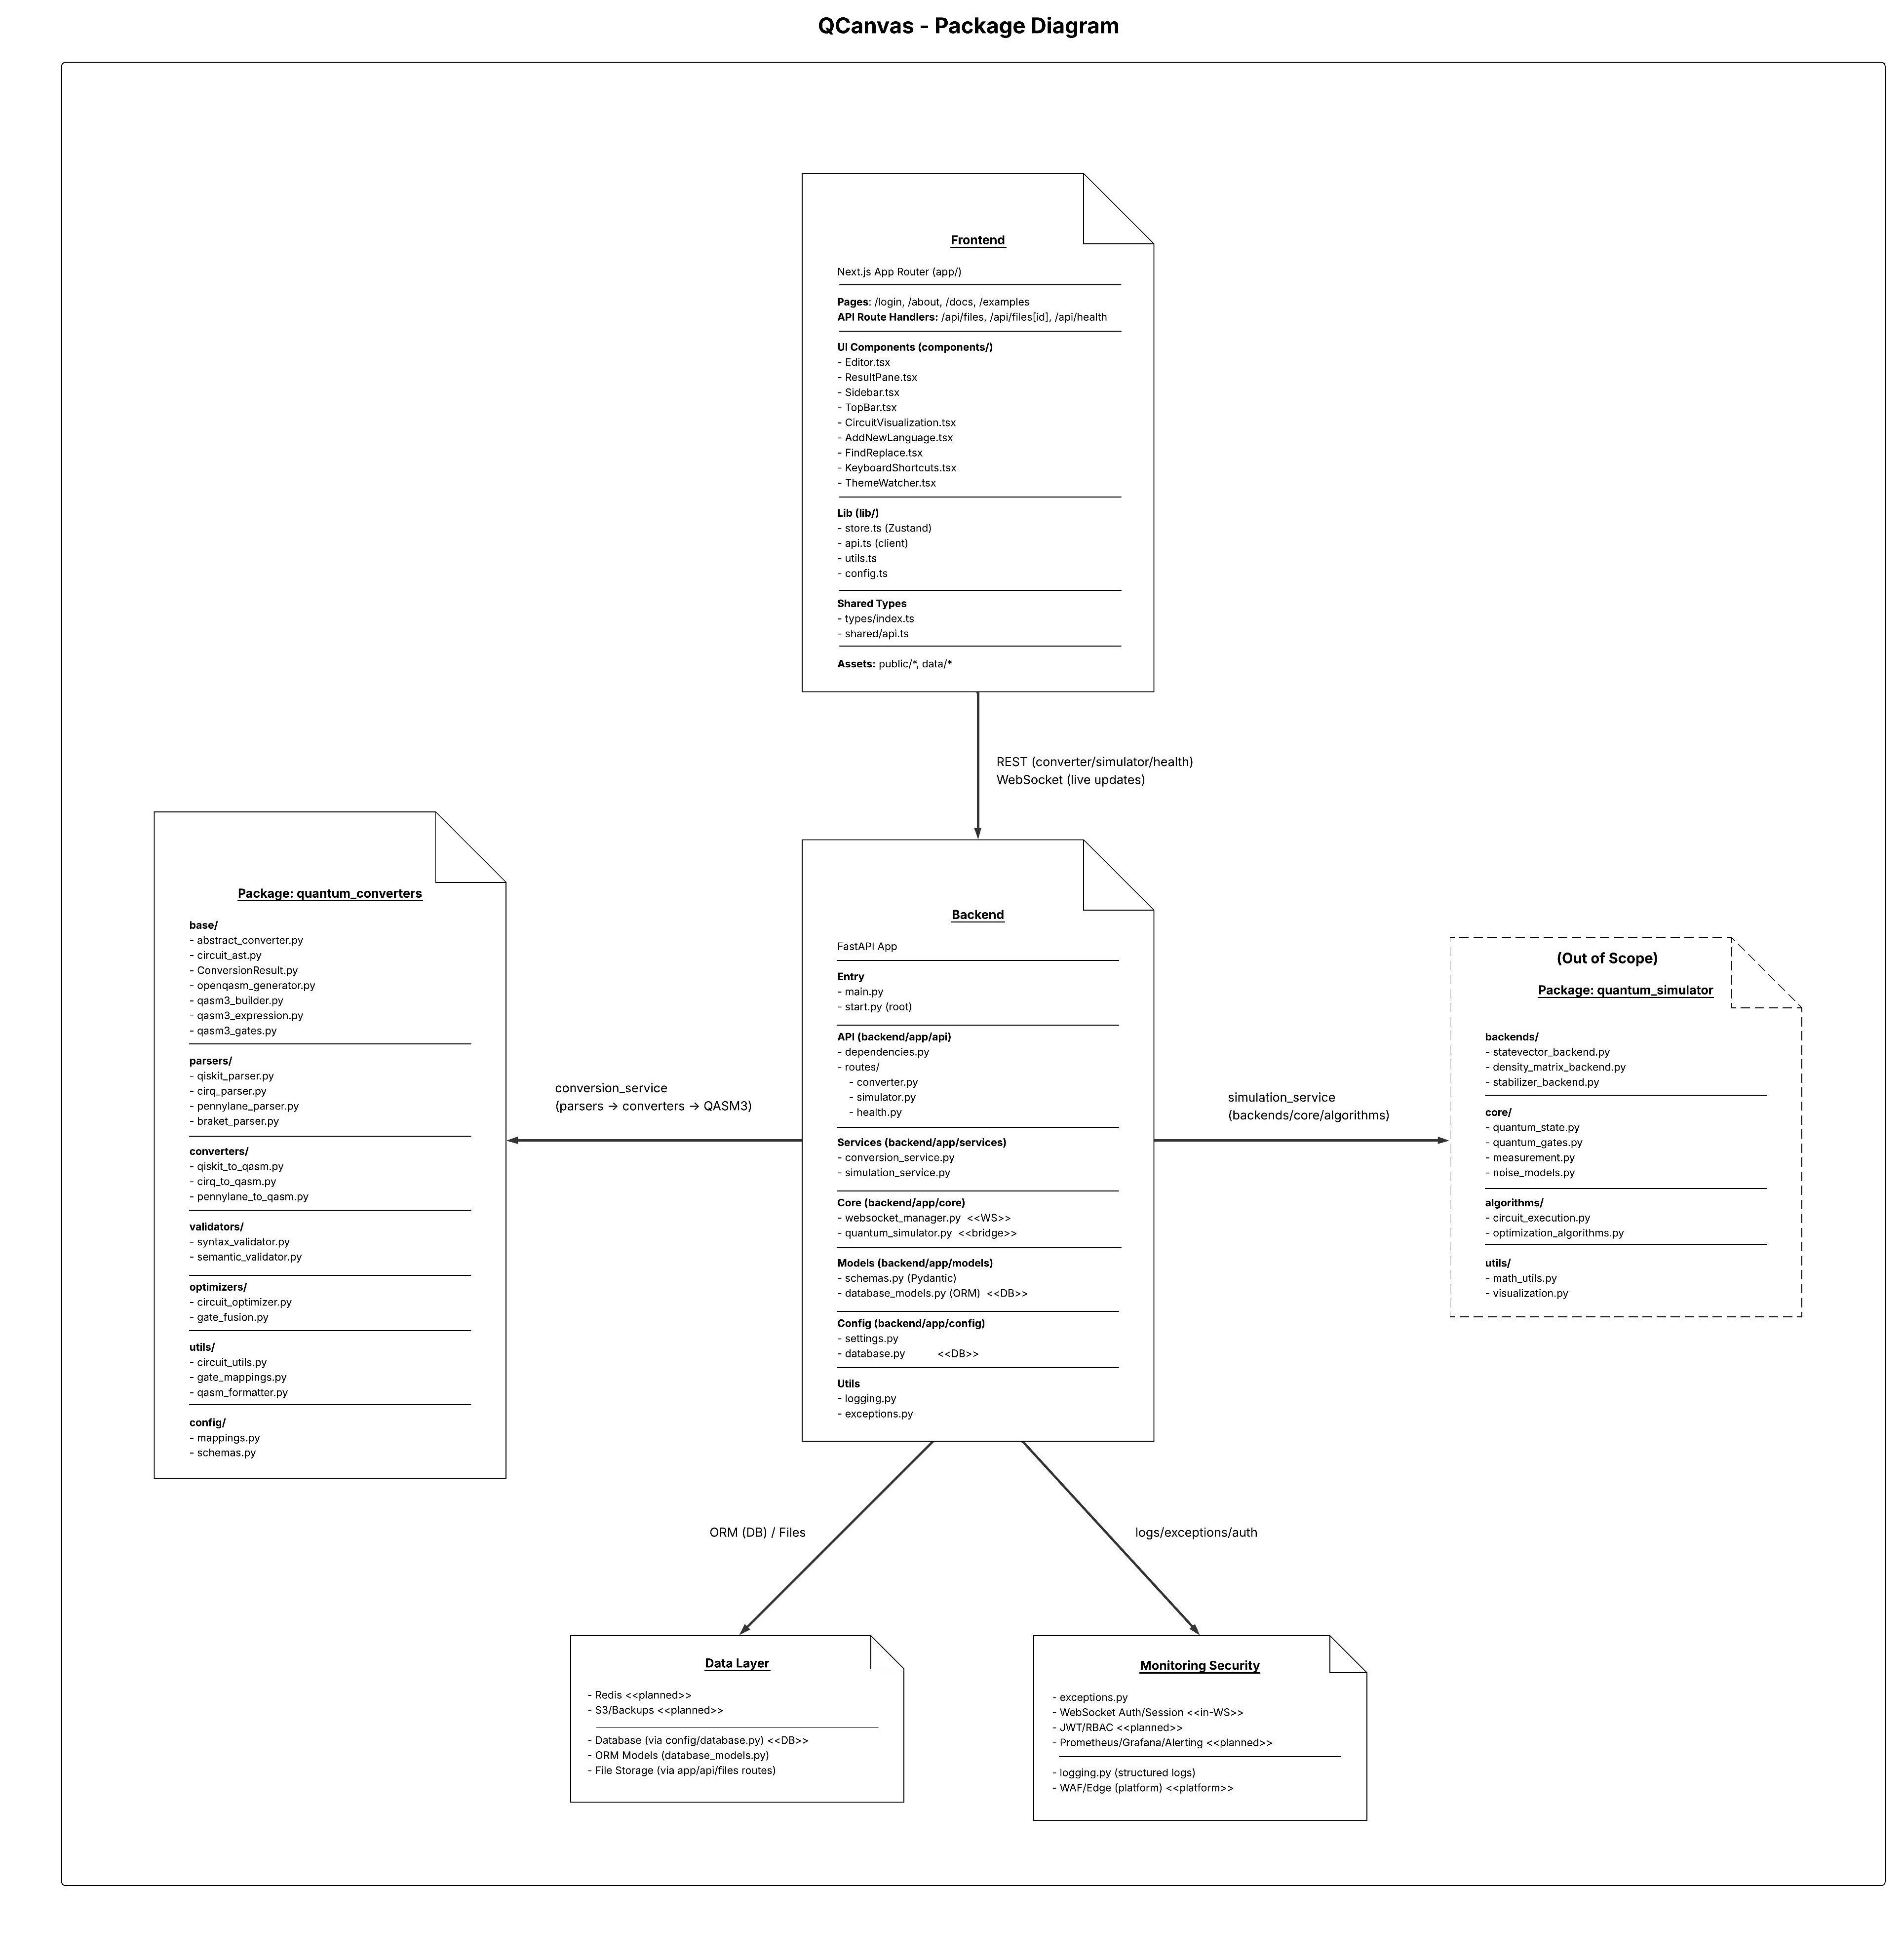
\includegraphics[width=0.95\linewidth]{Package Diagram.jpeg}
    \caption{Package Diagram}
    \label{fig:package}
\end{figure}

\clearpage
\subsection{Deployment Diagram}
This diagram shows the deployment view for production: an Nginx HTTP reverse proxy, the FastAPI backend service, the Next.js frontend, PostgreSQL/Redis containers, and containerization via Docker Compose.
\begin{figure}[H]
    \centering
    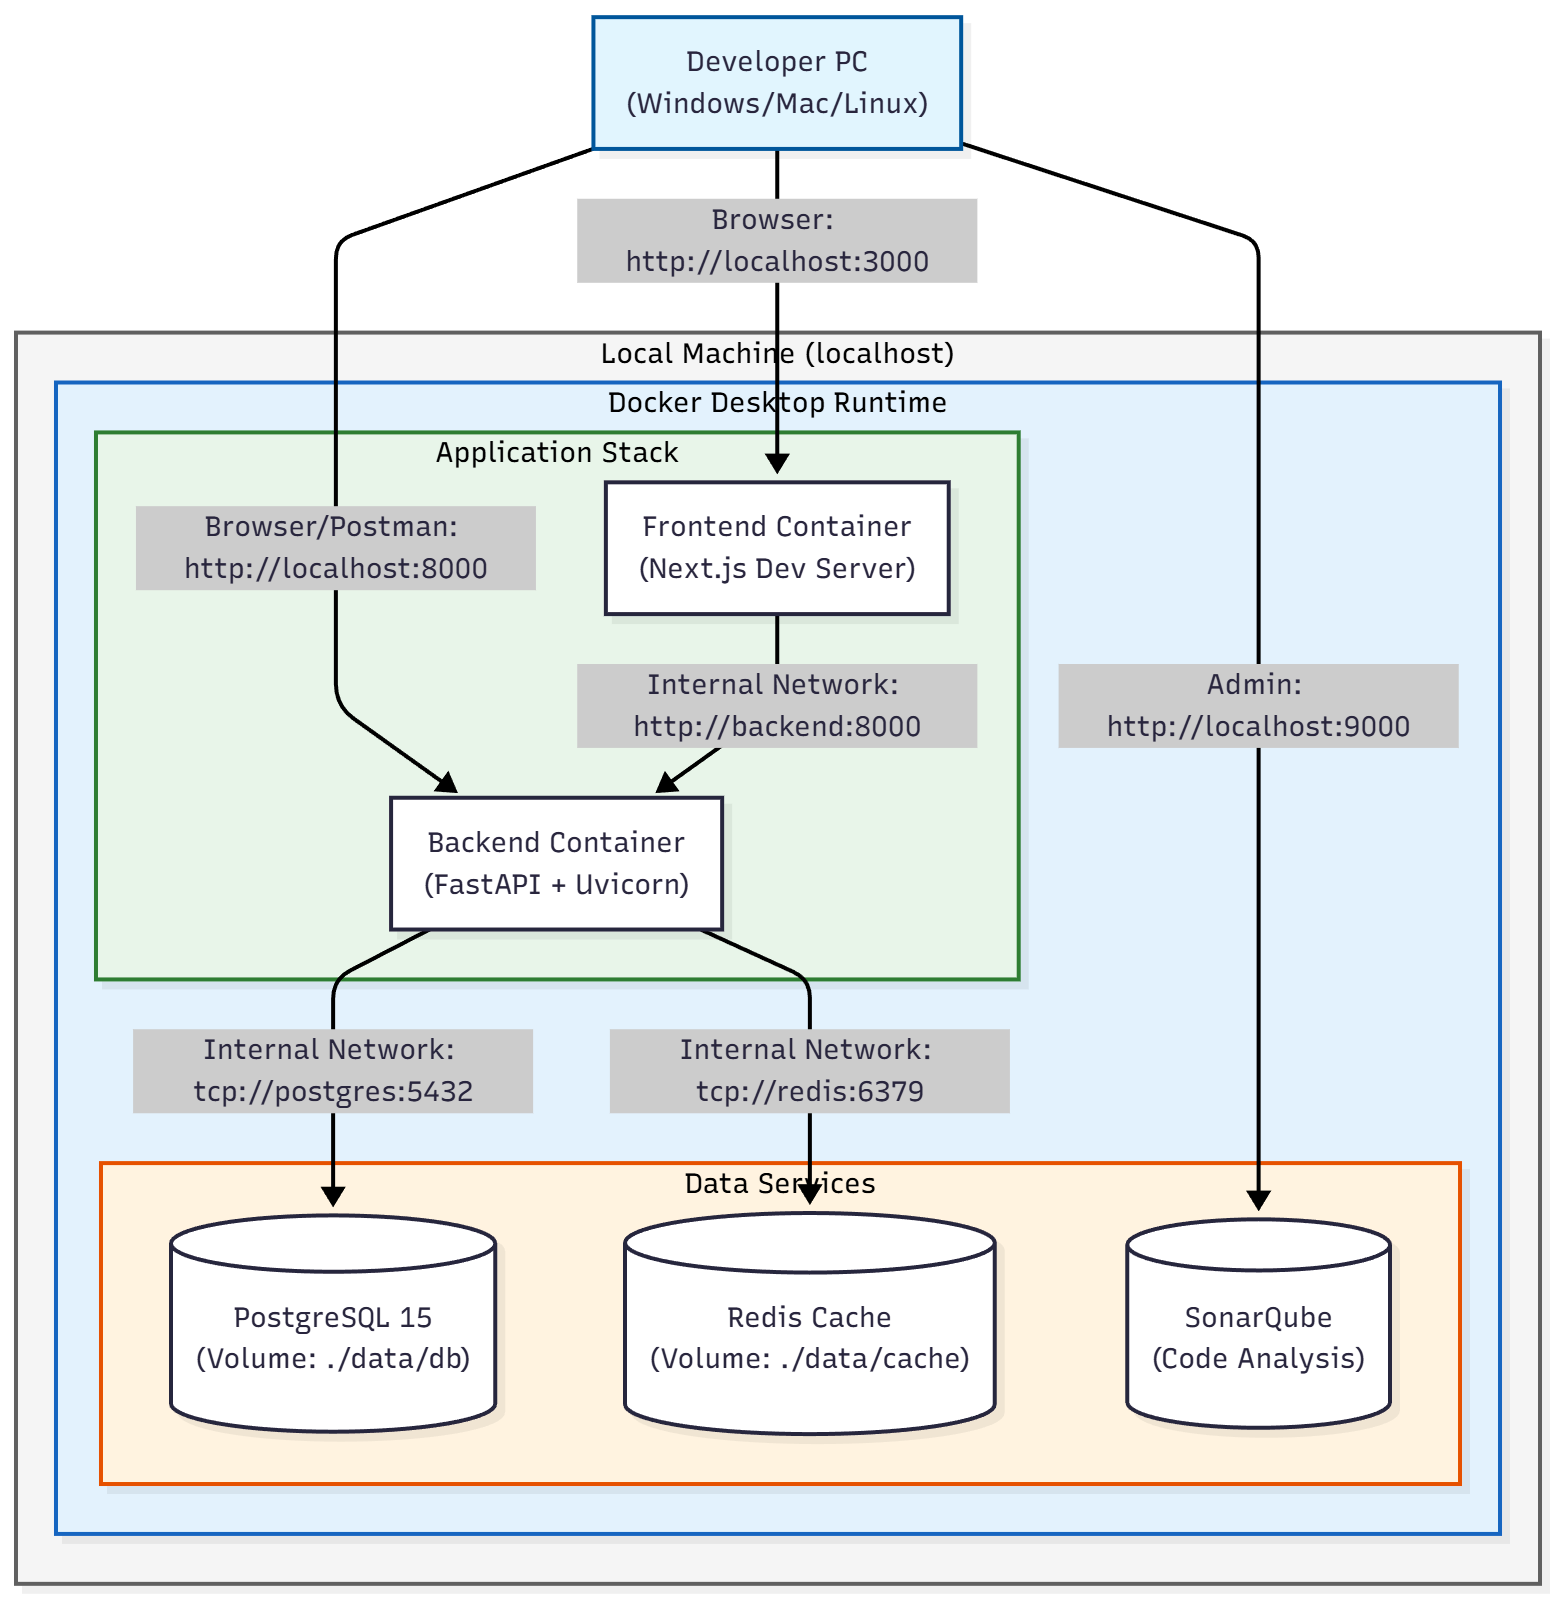
\includegraphics[width=0.95\linewidth]{FYP-Deployment.png}
    \caption{Deployment Diagram}
    \label{fig:deployment}
\end{figure}

\clearpage
\subsection{State Diagrams}

\subsubsection{State Diagram: Conversion Process}
\begin{figure}[H]
    \centering
    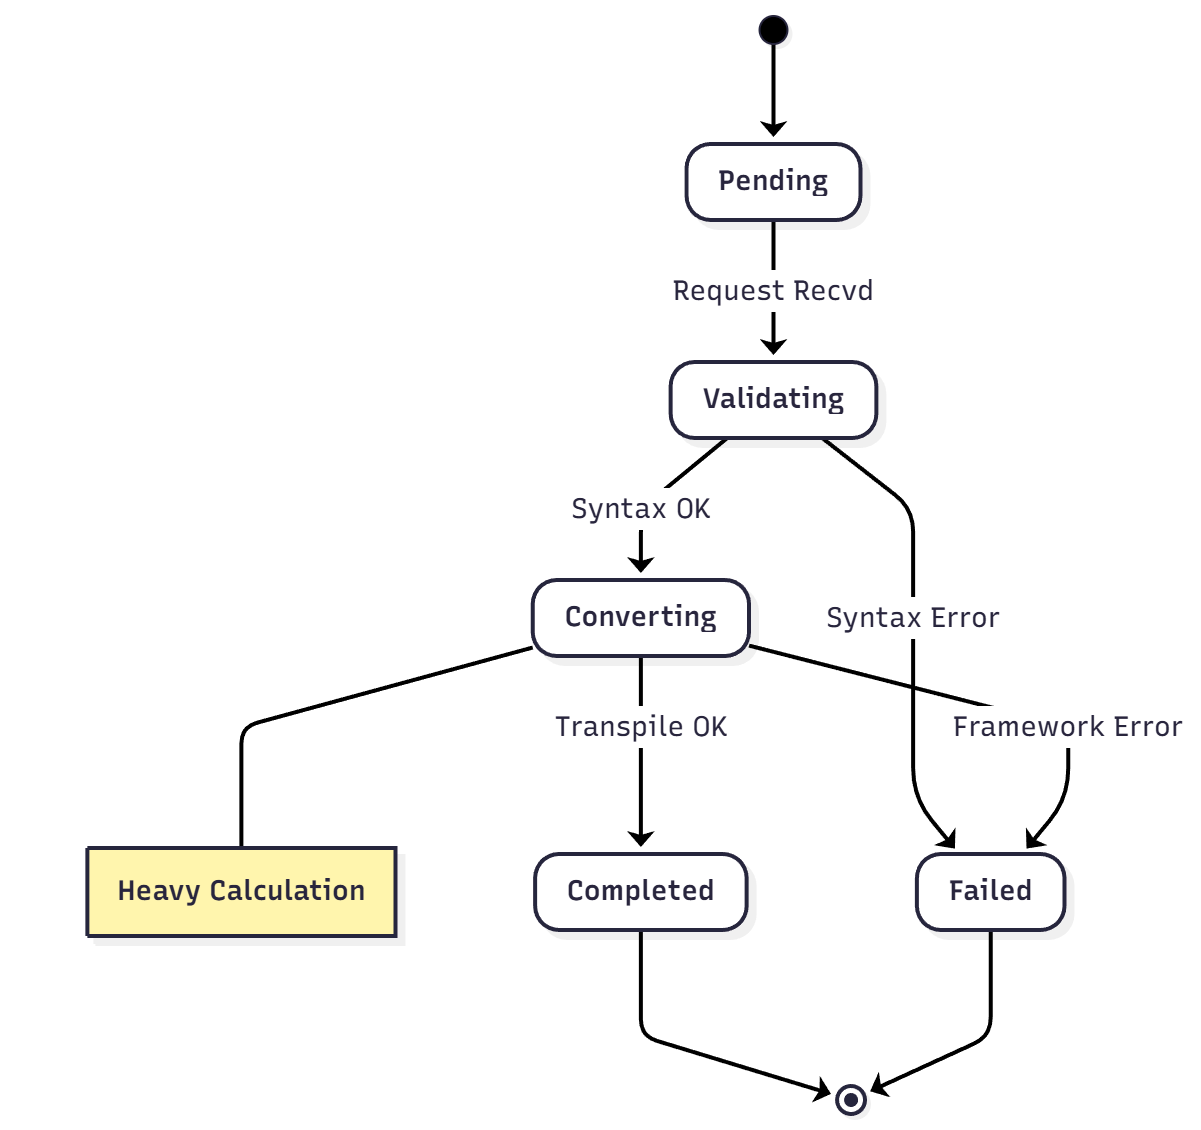
\includegraphics[width=0.8\linewidth]{FYP-StateConversion.png}
    \caption{State Diagram --- Conversion}
\end{figure}

\subsubsection{State Diagram: Simulation Job}
\begin{figure}[H]
    \centering
    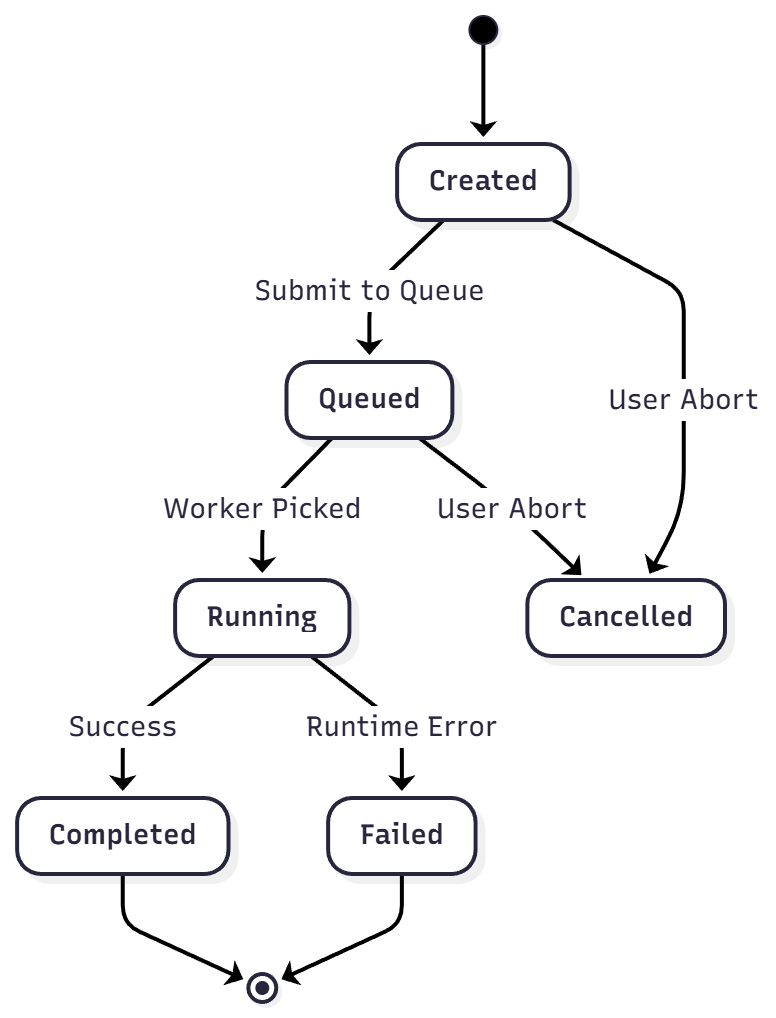
\includegraphics[width=0.8\linewidth]{FYP-StateJob.png}
    \caption{State Diagram --- Simulation Job}
\end{figure}

\clearpage
\subsection{Data Flow Diagrams (DFD)}

\subsubsection{DFD Level 0 (Context Diagram)}
At the context level, the DFD shows QCanvas as a single system interacting with external entities: the User, Authentication Provider, and QSim backend.
\begin{figure}[H]
    \centering
    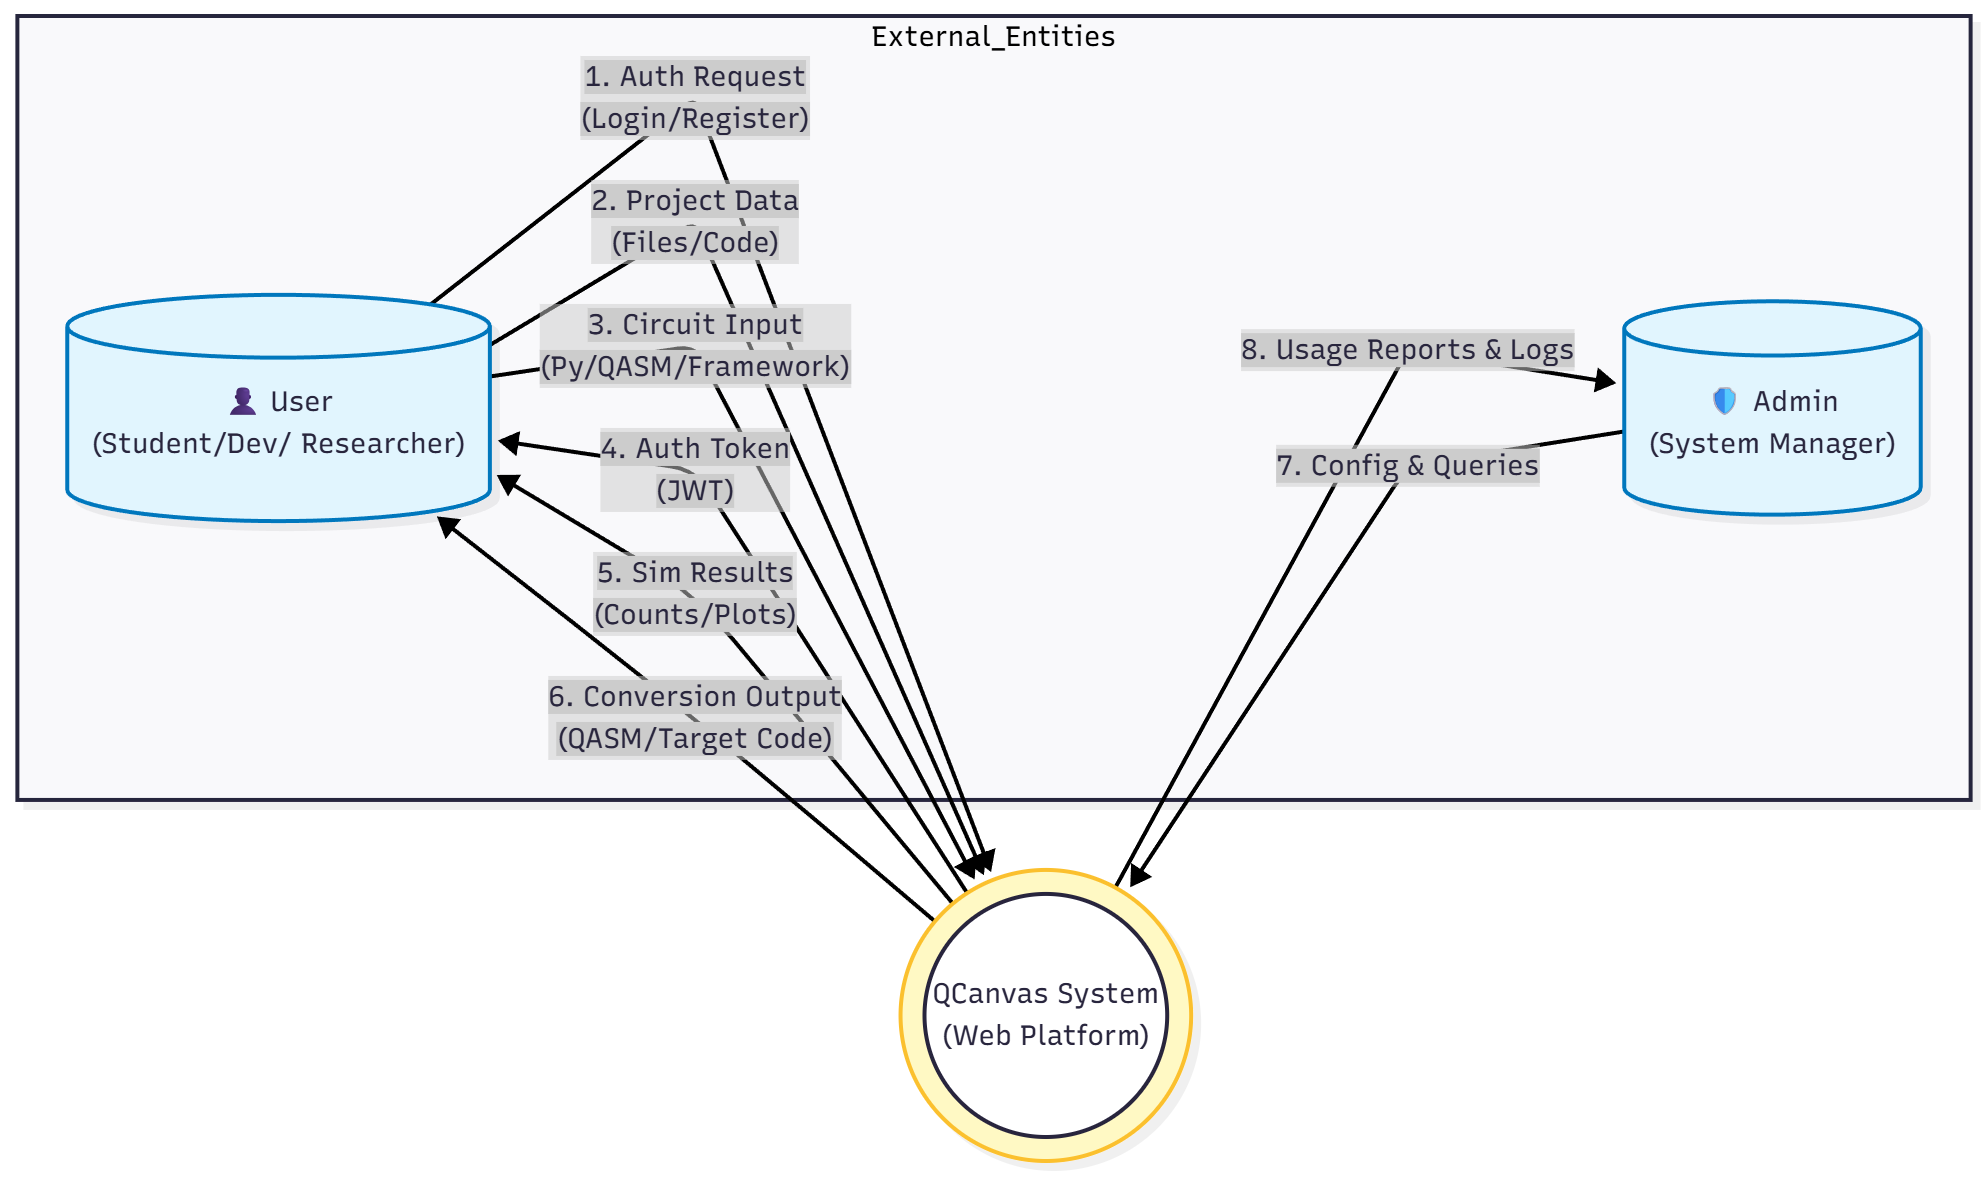
\includegraphics[width=0.8\linewidth]{FYP-DFD-lvl0.png}
    \caption{DFD Level 0}
\end{figure}

\subsubsection{DFD Level 1}
\begin{figure}[H]
    \centering
    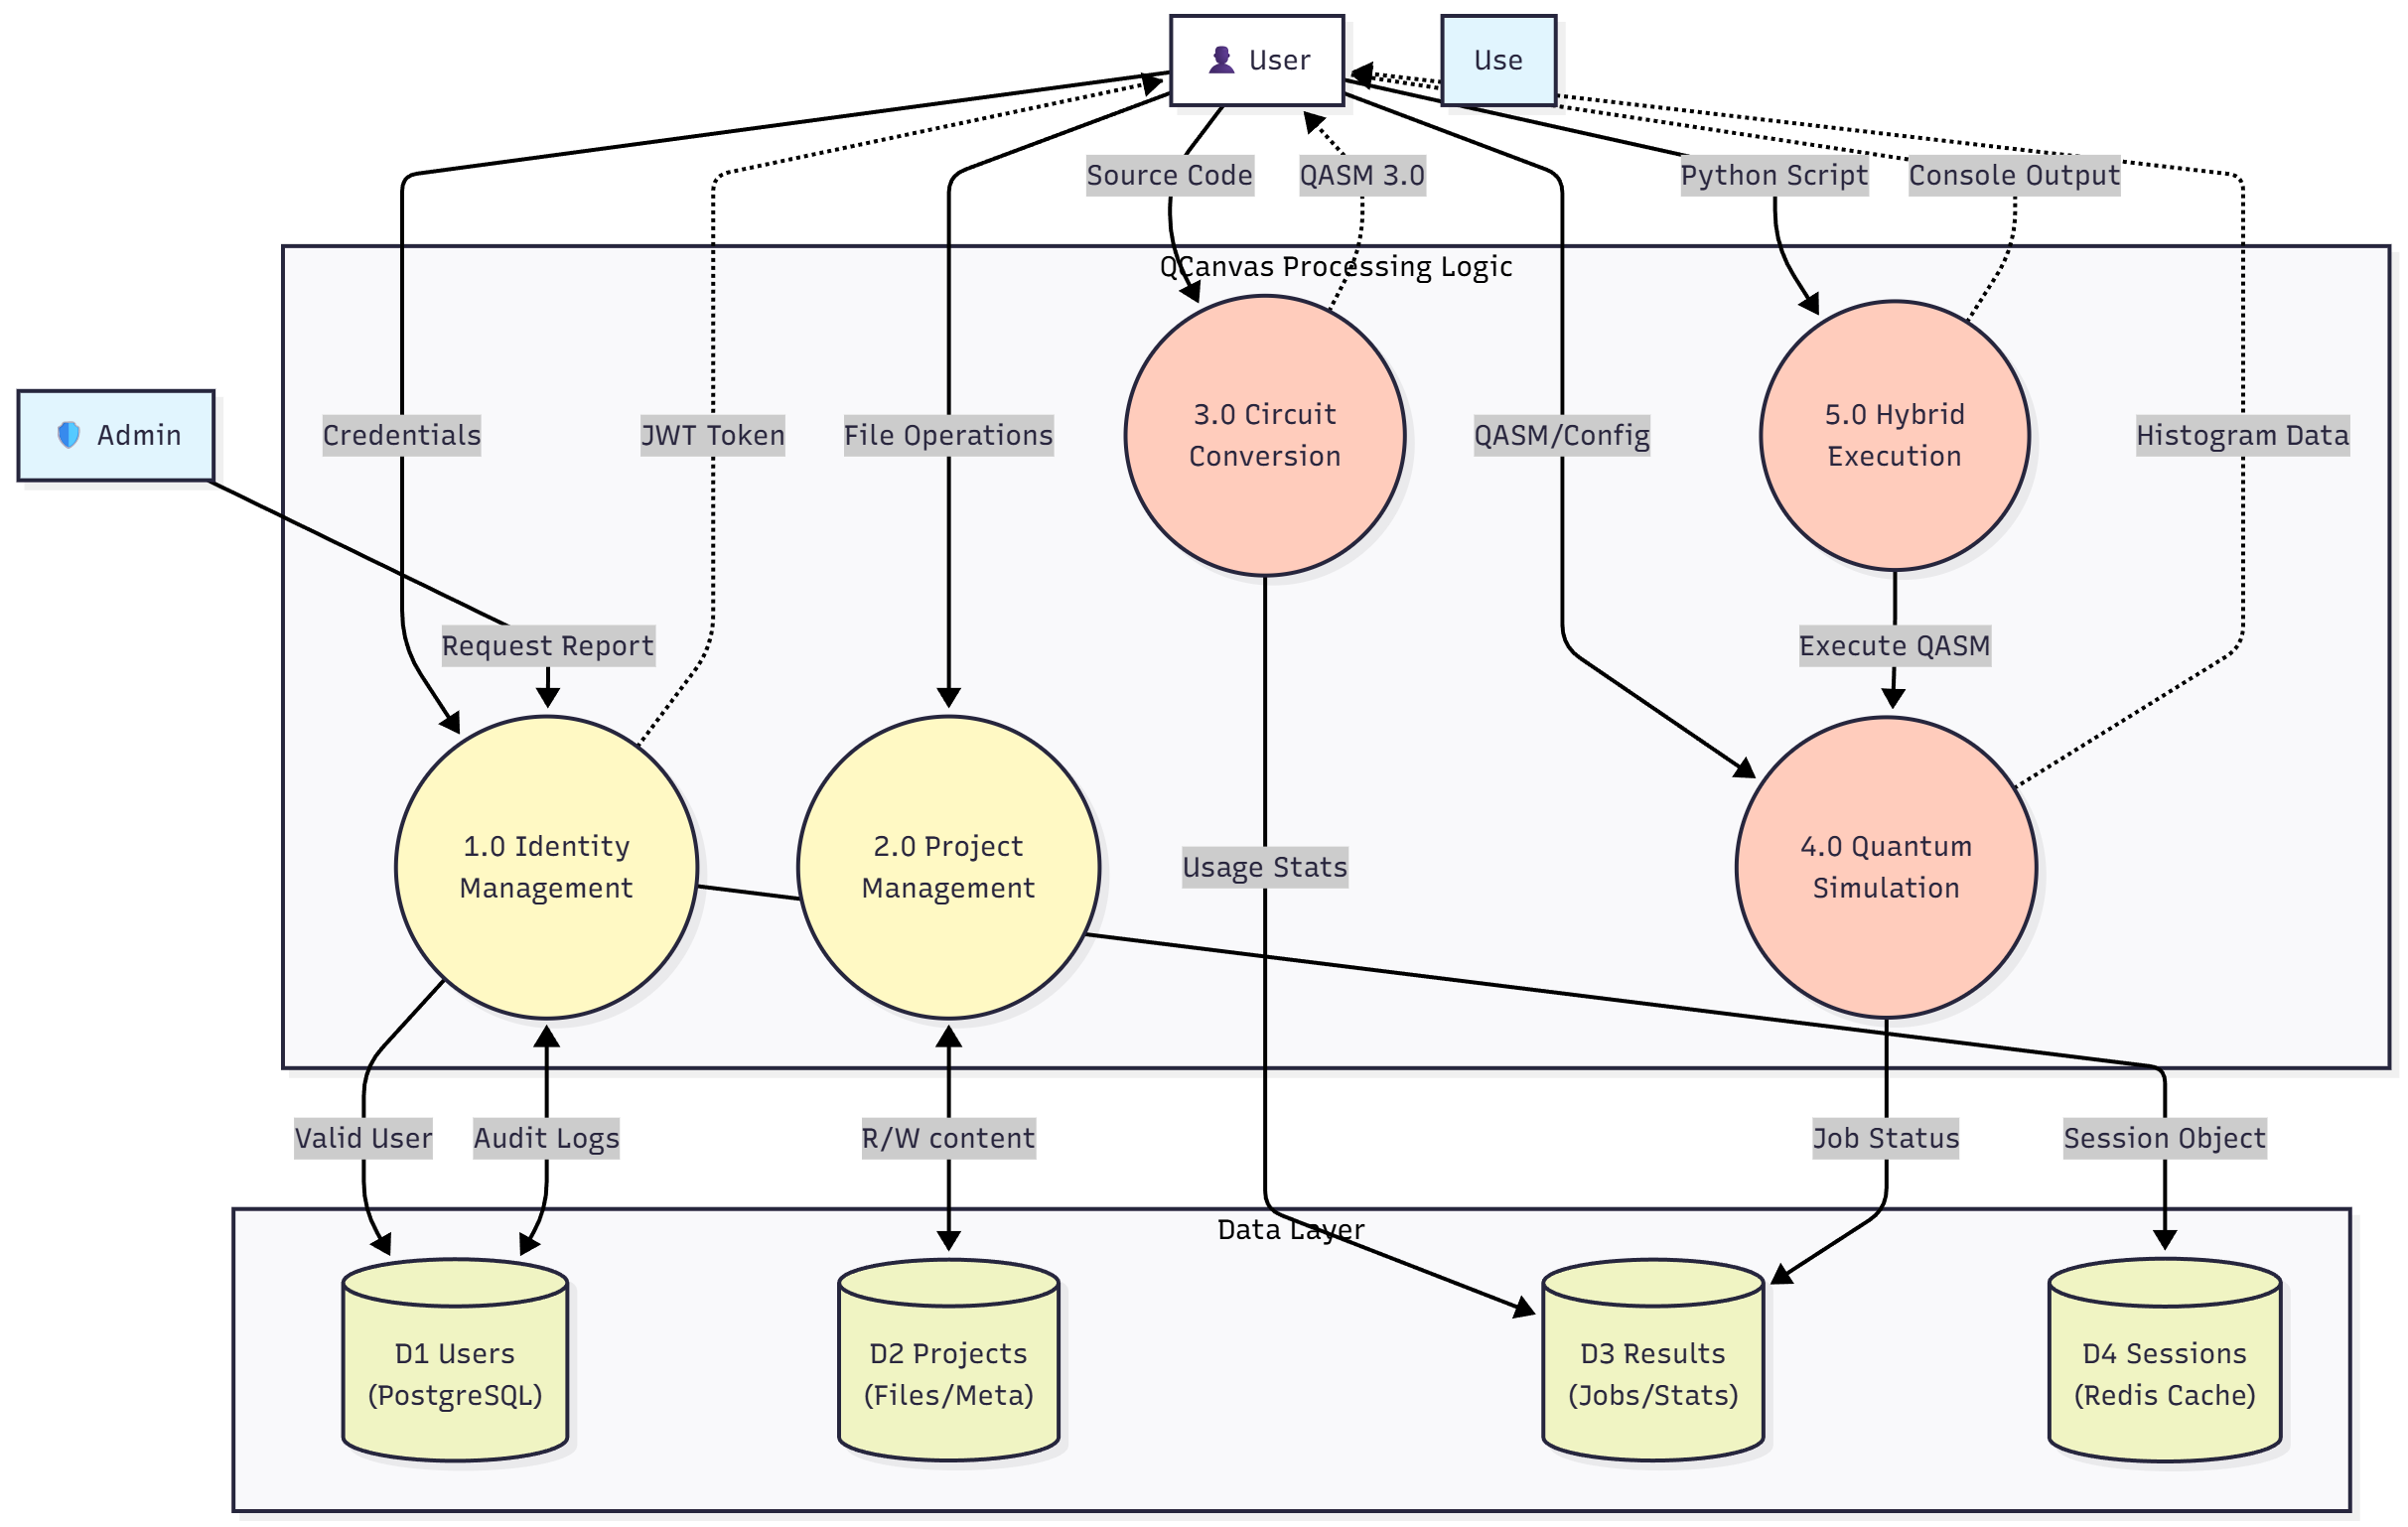
\includegraphics[width=0.98\linewidth]{FYP-DFD-lvl1.png}
    \caption{DFD Level 1}
\end{figure}

\section{Data Design}

\subsection{Core Entities}
\begin{itemize}
    \item \textbf{Circuit}: Framework source code, parsed AST, OpenQASM 3.0 representation, metadata, and statistics.
    \item \textbf{ConversionRequest}: Source framework, target framework or QASM, source code, optimization options, validation flags.
    \item \textbf{ConversionResult}: Generated OpenQASM 3.0 code, conversion statistics, warnings, errors, execution time.
    \item \textbf{SimulationJob}: OpenQASM code, selected backend, shots, seed, execution status, progress percentage.
    \item \textbf{SimulationResult}: Measurement counts, statevector/density matrix (optional), execution time, metadata.
    \item \textbf{Project}: Files collection, active file reference, project settings, theme preferences.
    \item \textbf{User}: Authentication credentials, profile data, XP, level, achievement set.
    \item \textbf{Achievement}: Criteria type, threshold value, XP reward, unlock state.
    \item \textbf{Recipe}: Circuit snippet, framework tag, difficulty label, community tags, upvote count.
\end{itemize}

\subsection{Entity Relationship Diagram}
\begin{figure}[H]
    \centering
    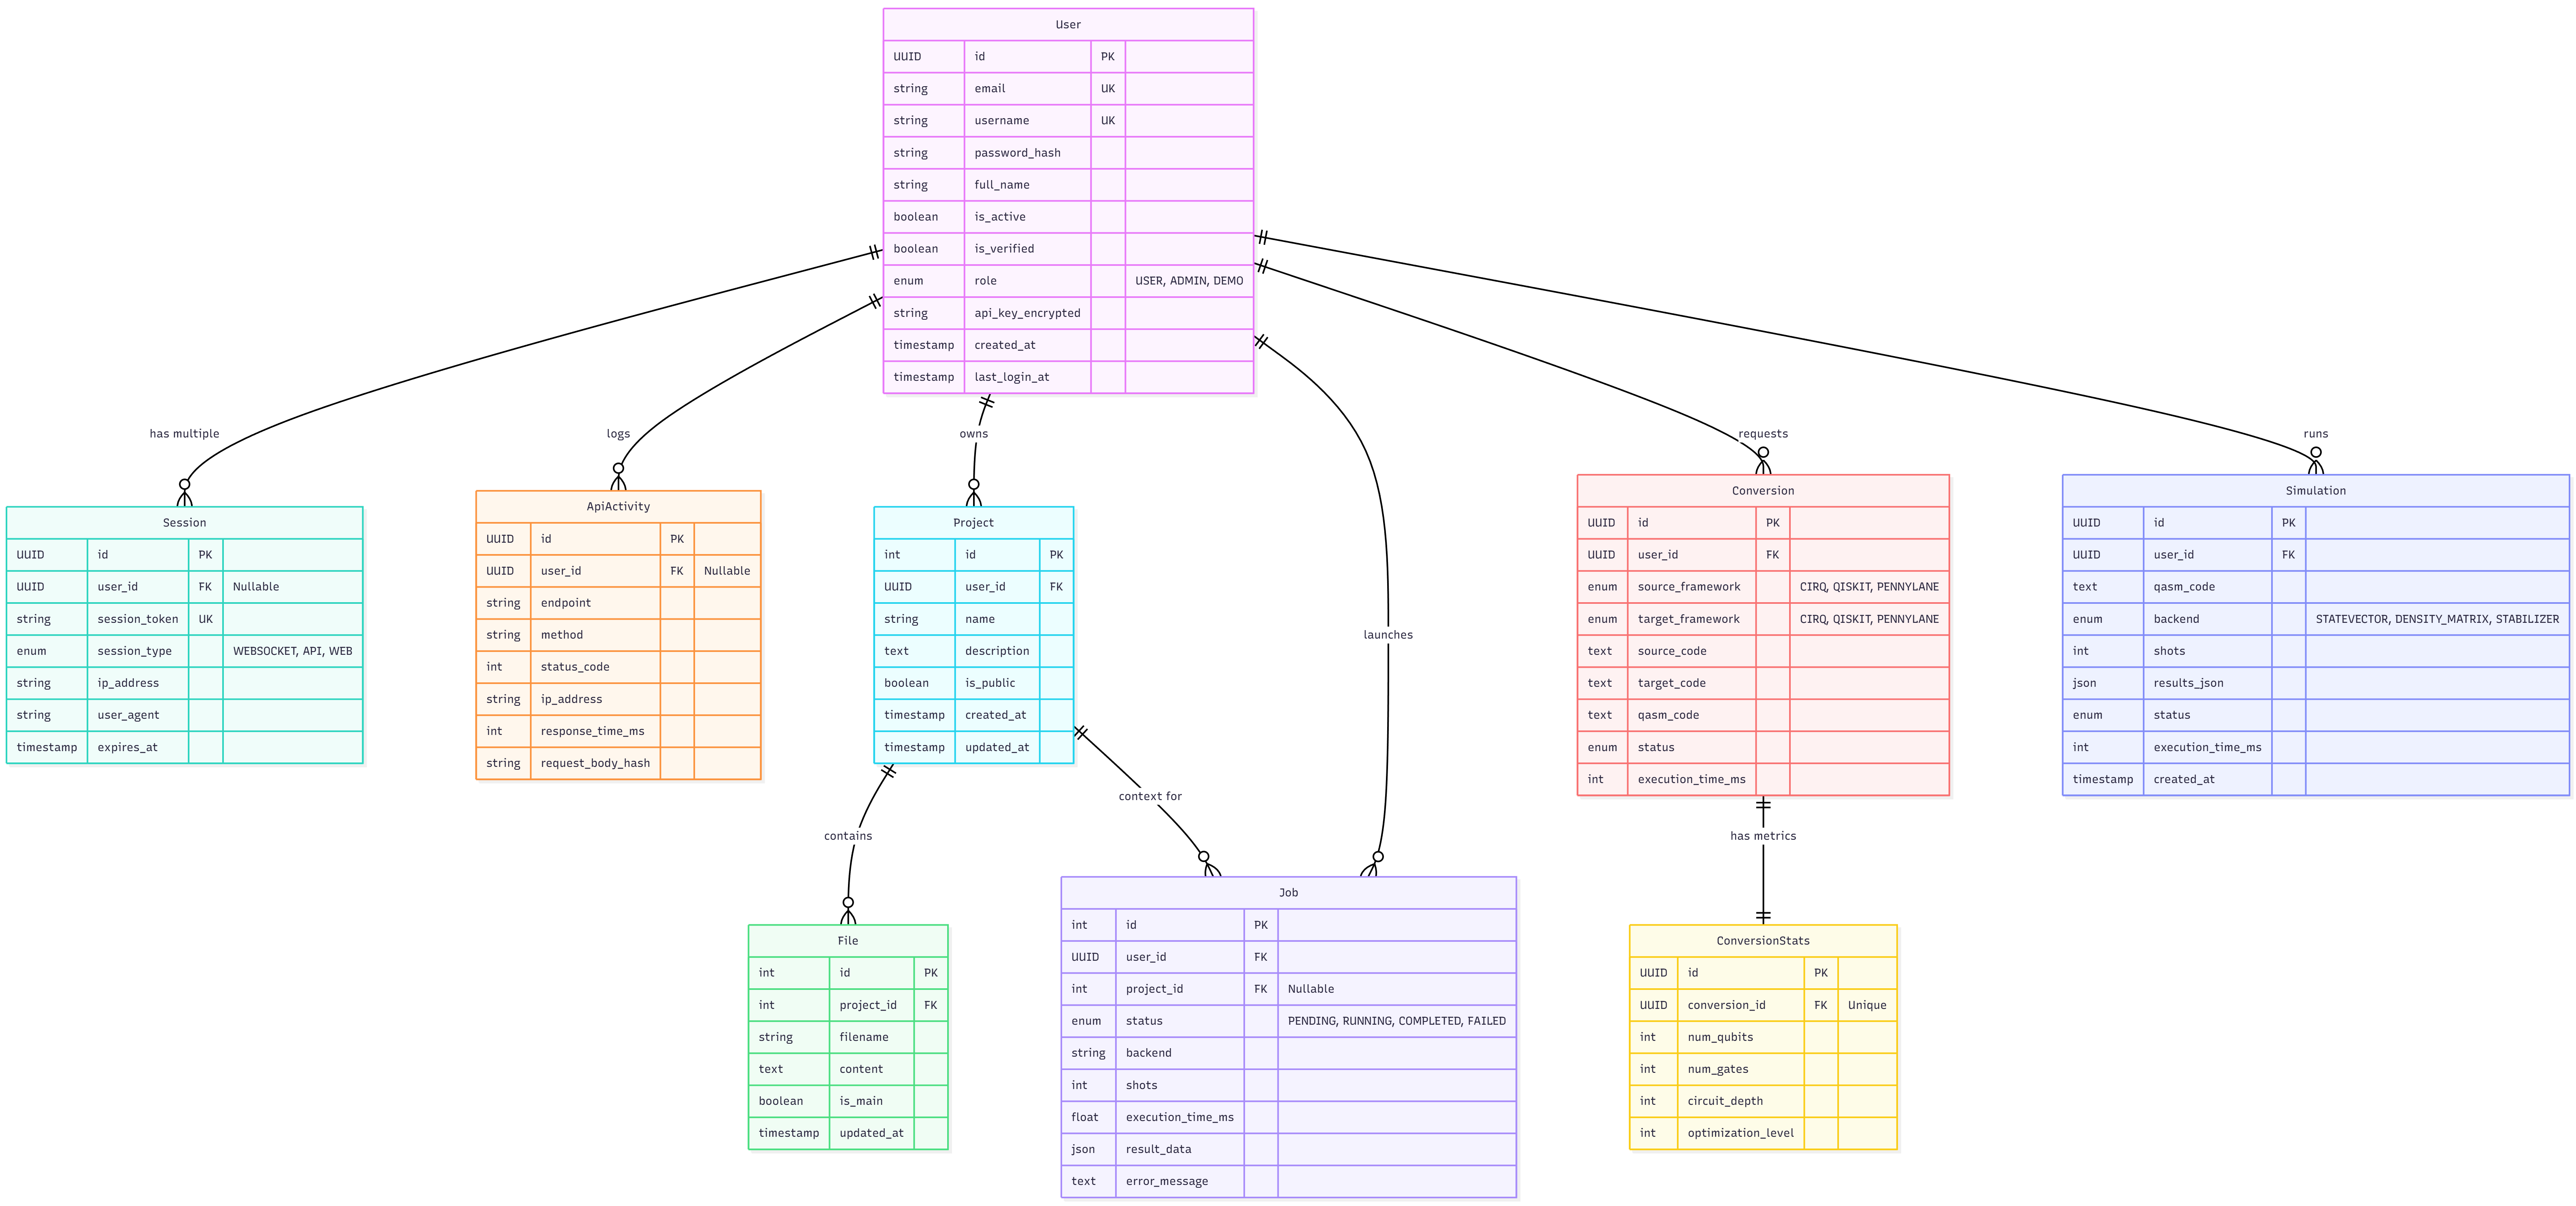
\includegraphics[width=\linewidth]{FYP-ErdDiagram.png}
    \caption{Entity Relationship Diagram}
    \label{fig:erd}
\end{figure}

\subsection{Data Organization and Processing}

\begin{longtable}{p{0.22\textwidth} p{0.70\textwidth}}
\toprule
\textbf{Layer} & \textbf{Data Handled / Description} \\
\midrule
\endfirsthead
\toprule
\textbf{Layer} & \textbf{Data Handled / Description} \\
\midrule
\endhead
Input Layer & Source code (Python/QASM), examples, editor configuration (JSON), user preferences \\
Parsing Layer & Python AST, circuit operations, gate definitions, qubit mappings \\
Conversion Layer & CircuitAST intermediate format, gate mappings, OpenQASM 3.0 text, diagnostics \\
Validation Layer & Syntax errors, semantic errors, unsupported feature warnings, subset conformance checks \\
Simulation Layer & Backend selection, shots configuration, execution parameters, caching keys \\
Results Layer & Measurement counts, histograms, statevector arrays, execution metadata \\
Rendering Layer & Circuit diagrams (SVG/D3), charts (Chart.js), formatted statistics \\
Persistence Layer & Project files, conversion history, results cache, user sessions, achievements, recipes \\
\bottomrule
\caption{Data Organization and Processing}
\label{tab:data-organization}
\end{longtable}

\subsection{API Data Models}

All API endpoints use Pydantic models for validation:

\subsubsection{Request Models}
\begin{itemize}
    \item \texttt{ConversionRequest}: source\_framework, target\_framework, source\_code, style, validate
    \item \texttt{SimulationRequest}: qasm\_code, backend, shots, seed, noise\_model
    \item \texttt{FileRequest}: name, content, language, project\_id
    \item \texttt{RecipeRequest}: title, code, framework, difficulty, tags
\end{itemize}

\subsubsection{Response Models}
\begin{itemize}
    \item \texttt{ConversionResponse}: success, qasm\_code, stats, warnings, errors, timestamp
    \item \texttt{SimulationResponse}: success, results, execution\_time, backend\_info, timestamp
    \item \texttt{ErrorResponse}: error\_code, message, details, suggestions
    \item \texttt{AchievementEvent}: achievement\_id, name, xp\_awarded, new\_level
\end{itemize}

\chapter{Implementation and Testing}
\label{ch:implementation}

This chapter details the implementation progress across all four iterations, the algorithm design, external APIs, testing results, and the full cross-framework benchmarking evaluation.

\section{Algorithm Design}

The core pipeline of QCanvas is its multi-stage quantum circuit compilation algorithm. The pseudocode below describes the main conversion flow.

\begin{algorithm}[H]
\caption{QCanvas Circuit Compilation Pipeline}
\begin{algorithmic}[1]
\Require Source code $S$, framework $F$, backend $B$, shots $n$
\Ensure Measurement counts $C$, execution metadata $M$

\State $F \gets \textsc{DetectFramework}(S)$  \Comment{Inspect imports and class patterns}
\State $\text{AST} \gets \textsc{ParseAST}(S, F)$  \Comment{AST traversal; runtime fallback if ambiguous}
\State $\text{ops} \gets \textsc{ExtractOps}(\text{AST})$  \Comment{Gate list, qubits, params, measurements}
\State $\text{QASM} \gets \textsc{QASM3Builder.build}(\text{ops})$  \Comment{Header + declarations + gates}
\State $\text{diag} \gets \textsc{Validate}(\text{QASM})$  \Comment{Subset check; emit line-precise errors}
\If{$\text{diag.has\_errors}$}
    \State \Return $\text{diag}$  \Comment{Return diagnostics to frontend; halt}
\EndIf
\State $\text{job} \gets \textsc{QSim.submit}(\text{QASM}, B, n)$  \Comment{Dispatch to selected backend}
\State $C, M \gets \textsc{QSim.collect}(\text{job})$  \Comment{Counts, exec time, state snapshot}
\State \Return $C, M$
\end{algorithmic}
\end{algorithm}

\section{External APIs and SDKs}

\begin{table}[!h]
\resizebox{\textwidth}{!}{%
\begin{tabular}{|p{3cm}|p{4cm}|p{4cm}|p{4cm}|}
\hline
\textbf{API / SDK} & \textbf{Description} & \textbf{Purpose} & \textbf{Key Interface} \\ \hline
Qiskit (v0.44+) & IBM quantum framework & Parse/convert Qiskit circuits to OpenQASM 3.0 & \texttt{QuantumCircuit} \cite{qiskit} \\ \hline
Cirq (v1.0+) & Google quantum framework & Parse/convert Cirq circuits & \texttt{cirq.Circuit} \cite{cirq_developers_2023} \\ \hline
PennyLane (v0.33+) & Xanadu variational framework & Parse/convert PennyLane QNodes & \texttt{qml.QNode} \cite{bergholm2018pennylane} \\ \hline
QSim SDK (PyPI) & Custom simulation kernel & Execute OpenQASM 3.0 circuits & \texttt{StatevectorBackend.run()} \cite{qsim_sdk_2026} \\ \hline
FastAPI (v0.110+) & Async Python web framework & REST and WebSocket API & \texttt{APIRouter}, \texttt{WebSocket} \\ \hline
Monaco Editor & Microsoft in-browser IDE & Syntax highlighting, hover providers & \texttt{editor.create()} \\ \hline
D3.js (v7) & SVG data-driven library & Real-time 2D circuit diagram & \texttt{d3.select}, \texttt{d3.join()} \\ \hline
PostgreSQL/SQLAlchemy & Relational DB + ORM & Persistent storage for all entities & \texttt{Session}, \texttt{Base.metadata} \\ \hline
\end{tabular}%
}
\caption{External APIs and SDKs Used}
\label{tab:external-apis}
\end{table}

\section{Iteration-by-Iteration Implementation Progress}

\subsection{Iteration 1: Core Infrastructure and Basic Features}
Iteration 1 established the foundational architecture: FastAPI backend, Next.js 14 frontend with TypeScript and Tailwind CSS, Docker Compose DevOps, and initial Cirq/Qiskit/PennyLane to OpenQASM 3.0 conversion with standard gates, if-else control flow, and the complete OpenQASM 3.0 type system \cite{cross2021openqasm}.

\subsection{Iteration 2: Advanced Features and Hybrid Execution}
Iteration 2 added advanced OpenQASM 3.0 constructs (\texttt{while}, \texttt{break}, \texttt{continue}, subroutines, complex types, bitwise operators), expanded PennyLane gate coverage (CY, CH, CRX, CRY, CRZ, CP, CSWAP, CCZ, GlobalPhase, \texttt{negctrl}, \texttt{ctrl(n)}, \texttt{pow(k)}), the full database layer (SQLAlchemy models, Alembic migrations, FK constraints), and the hybrid CPU--QPU execution model separating classical orchestration from QSim-powered quantum execution. Security was hardened with AES-256 key encryption, Bcrypt password hashing, and RBAC.

\subsection{Iteration 3: Educational Intelligence and Community Features}
Iteration 3 delivered the real-time D3.js circuit visualisation pipeline with 500ms debounce, the ``Quantum Explain It'' hover system, an event-driven gamification engine with 44 unique achievements and XP progression to Level~50+, and the community recipe-sharing platform. The plug-in language architecture was reinforced with Monarch tokenizer injection for \texttt{qasm} and \texttt{pythonq} language modes.

\subsection{Iteration 4: QSim SDK Integration, Benchmarking, and PyPI Deployment}
Iteration 4 marks the project's completion. Both the QCanvas converter SDK and the QSim simulation SDK were packaged and deployed to PyPI:
\begin{itemize}
    \item \texttt{pip install qsim-sdk} --- standalone quantum simulation engine.
    \item \texttt{pip install qcanvas-sdk} --- Qiskit/Cirq/PennyLane to OpenQASM 3.0 converter.
\end{itemize}
The example library was expanded to 40+ categorised algorithms. A comprehensive cross-framework benchmarking study was conducted and a Docker Compose production deployment with Nginx reverse proxy was finalised.

\section{User Interface Implementation}

The QCanvas Web IDE, delivered across all four iterations, provides:
\begin{itemize}
    \item Monaco editor with custom syntax highlighting and hover-based quantum explanations.
    \item Real-time D3.js 2D circuit diagram (debounced) and 3D visualisation via \texttt{@react-three/fiber}.
    \item Chart.js measurement histograms, statevector tables, and execution statistics.
    \item Achievement dashboard with XP bar, level display, and badge collection.
    \item Community library with recipe browsing, forking, and tag-based filtering.
    \item Full dark and light theme support.
\end{itemize}

\section{Testing and Validation}

\subsection{Testing Strategy}
The verification approach combines three layers: (1) backend regression tests covering the converter, simulator, database layer, and authentication flows; (2) targeted feature checks for Iterations 3 and 4; and (3) manual exploratory testing for visual behaviour (circuit rendering, gamification progression).

\subsection{Unit Testing}
Unit tests validate: conversion correctness for all supported gates across Cirq, Qiskit, and PennyLane; OpenQASM 3.0 output validity; QSim simulation correctness against known quantum state distributions; authentication and RBAC logic; and gamification achievement criteria.

\subsection{Test Coverage}

\begin{table}[H]
\centering
\caption{Test Coverage Summary}
\label{tab:test-coverage}
\begin{tabular}{|l|r|l|}
\hline
\textbf{Iteration / Suite} & \textbf{Tests} & \textbf{Scope} \\ \hline
Iteration 1 & 73 & Basic conversion, gates, type system \\ \hline
Iteration 2 & 151 & Advanced features, DB models, auth, RBAC \\ \hline
Integration Tests & 80 & End-to-end conversion and hybrid execution \\ \hline
\textbf{Total} & \textbf{304} & \textbf{100\% pass rate} \\ \hline
\end{tabular}
\end{table}

\textit{Note: Iterations 3 and 4 feature additions (gamification service, recipe sharing, SDK packaging) were validated via manual exploratory testing and integration test extensions included in the 80 integration tests above.}

\section{Evaluation and Benchmarking}

Iteration 4 delivered a reproducible benchmarking study titled \textit{``Cross-Framework Quantum Algorithm Benchmarking via Unified Compilation to OpenQASM 3.0''}, using QCanvas as the compilation platform and QSim as the execution engine.

\subsection{Benchmark Setup}
\begin{itemize}
    \item \textbf{Environment:} Windows 11, Intel Core i7, 16 GB RAM, Python 3.11.
    \item \textbf{Algorithm Suite:} 12 standard algorithms (Bell State, GHZ State, Quantum Teleportation, Deutsch--Jozsa, Bernstein--Vazirani, Grover's Algorithm, QRNG, VQE, QAOA, QML XOR Classifier, Bit-Flip Code, Phase-Flip Code).
    \item \textbf{Frameworks:} Qiskit, Cirq, PennyLane --- each with idiomatic native implementations.
    \item \textbf{Qubit Range:} 2--8 qubits per algorithm; 136 distinct configurations.
    \item \textbf{Shots:} 4,096 per simulation run; 10 runs per configuration for statistical robustness.
\end{itemize}

\subsection{Compilation Time Results}

Table~\ref{tab:compile-times} shows mean compilation latency (ms) for representative algorithms. All values are well within the NFR-P1 target of 1500ms.

\begin{table}[H]
\centering
\caption{Mean Compilation Latency (ms) -- Representative Algorithms at 8 Qubits}
\label{tab:compile-times}
\resizebox{\textwidth}{!}{%
\begin{tabular}{|l|r|r|r|}
\hline
\textbf{Algorithm} & \textbf{Qiskit (ms)} & \textbf{Cirq (ms)} & \textbf{PennyLane (ms)} \\ \hline
Bell State & 18.6 $\pm$ 0.4 & 8.3 $\pm$ 0.5 & 12.2 $\pm$ 0.3 \\ \hline
GHZ State & 21.9 $\pm$ 0.9 & 10.7 $\pm$ 0.4 & 38.0 $\pm$ 0.9 \\ \hline
Bernstein--Vazirani & 17.5 $\pm$ 0.6 & 13.0 $\pm$ 0.5 & 98.9 $\pm$ 2.5 \\ \hline
Deutsch--Jozsa & 7.0 $\pm$ 0.3 & 12.1 $\pm$ 1.3 & 106.3 $\pm$ 3.4 \\ \hline
Grover's Algorithm & 9.6 $\pm$ 0.5 & 32.5 $\pm$ 1.9 & 184.2 $\pm$ 6.5 \\ \hline
VQE & 32.9 $\pm$ 3.9 & 13.8 $\pm$ 1.0 & 55.2 $\pm$ 2.9 \\ \hline
QAOA & 55.0 $\pm$ 3.2 & 19.1 $\pm$ 2.6 & 73.7 $\pm$ 7.2 \\ \hline
\end{tabular}%
}
\end{table}

Cirq consistently achieves the lowest compilation latency (mean 8--35ms). PennyLane incurs the highest latency, exceeding 100ms for oracle-based algorithms due to its full gate decomposition strategy.

\subsection{Structural Benchmark Results}

\begin{table}[H]
\centering
\caption{Structural Benchmark Summary (Selected Algorithms)}
\label{tab:structural-summary}
\resizebox{\textwidth}{!}{%
\begin{tabular}{|l|l|r|r|r|r|}
\hline
\textbf{Algorithm} & \textbf{Framework} & \textbf{Qubits} & \textbf{Total Gates} & \textbf{Circuit Depth} & \textbf{Multi-Qubit Ratio} \\ \hline
Bell State & All Frameworks & 2 & 4 & 3 & 0.25 \\ \hline
\multirow{3}{*}{GHZ State} & Qiskit & 8 & 6 & 4 & 0.33 \\
 & Cirq & 8 & 6 & 4 & 0.33 \\
 & PennyLane & 8 & 16 & 9 & 0.44 \\ \hline
\multirow{3}{*}{Grover's Algorithm} & Qiskit & 6 & 18 & 12 & 0.11 \\
 & Cirq & 6 & 18 & 12 & 0.11 \\
 & PennyLane & 6 & 216 & 62 & 0.00 \\ \hline
\multirow{3}{*}{Bernstein--Vazirani} & Qiskit & 8 & 13 & 6 & 0.15 \\
 & Cirq & 8 & 13 & 6 & 0.15 \\
 & PennyLane & 8 & 31 & 4 & 0.16 \\ \hline
\multirow{3}{*}{VQE} & Qiskit & 6 & 5 & 2 & 0.20 \\
 & Cirq & 6 & 5 & 3 & 0.20 \\
 & PennyLane & 6 & 17 & 7 & 0.29 \\ \hline
\end{tabular}%
}
\end{table}

\begin{figure}[H]
    \centering
    
\includegraphics[width=0.90\linewidth]{fig02_gate_counts.png}
    \caption{Gate Count Comparison Across Frameworks}
    \label{fig:gate-counts}
\end{figure}

\begin{figure}[H]
    \centering
    
\includegraphics[width=0.90\linewidth]{fig03_circuit_depth.png}
    \caption{Circuit Depth Comparison Across Frameworks}
    \label{fig:circuit-depth}
\end{figure}

Qiskit and Cirq consistently produce structurally equivalent, compact circuits. PennyLane's default transpiler generates significantly more gates and deeper circuits for algorithms like Grover's (216 gates at 6 qubits vs.\ 18 for Qiskit/Cirq) due to its full-decomposition strategy for multi-qubit gates.

\subsection{Scaling Behaviour Analysis}

Power-law fits ($y = c \cdot n^a$) were computed for circuit depth as a function of qubit count. An exponent $a = 0$ indicates constant-depth scaling, optimal for NISQ execution.

\begin{table}[H]
\centering
\caption{Scaling Behaviour (Power-Law Fit: Circuit Depth vs.\ Qubits)}
\label{tab:scaling}
\begin{tabular}{|l|l|r|l|}
\hline
\textbf{Algorithm} & \textbf{Framework} & \textbf{Exponent ($a$)} & \textbf{Scaling Class} \\ \hline
GHZ State & Qiskit & 0.00 & Constant-depth \\
GHZ State & Cirq & 0.00 & Constant-depth \\
GHZ State & PennyLane & 1.00 & Linear \\ \hline
Deutsch--Jozsa & Qiskit & 0.00 & Constant-depth \\
Deutsch--Jozsa & Cirq & 0.00 & Constant-depth \\
Deutsch--Jozsa & PennyLane & 0.91 & Sub-linear \\ \hline
Grover's Algorithm & Qiskit & 0.00 & Constant-depth \\
Grover's Algorithm & Cirq & 0.00 & Constant-depth \\
Grover's Algorithm & PennyLane & 2.21 & Super-linear \\ \hline
Bernstein--Vazirani & Qiskit & 0.00 & Constant-depth \\
Bernstein--Vazirani & Cirq & 0.00 & Constant-depth \\
Bernstein--Vazirani & PennyLane & 0.87 & Sub-linear \\ \hline
\end{tabular}
\end{table}

\begin{figure}[H]
    \centering
    
\includegraphics[width=0.80\linewidth]{fig05_ghz_scaling.png}
    \caption{GHZ State Depth Scaling Across Frameworks}
    \label{fig:ghz-scaling}
\end{figure}

\begin{figure}[H]
    \centering
    
\includegraphics[width=0.80\linewidth]{fig14_grovers_scaling.png}
    \caption{Grover's Algorithm Depth Scaling --- PennyLane Super-Linear vs.\ Qiskit/Cirq Constant}
    \label{fig:grovers-scaling}
\end{figure}

\subsection{Statistical Equivalence Analysis}

Jensen--Shannon Divergence (JSD) was computed between pairwise output distributions to confirm that all three frameworks produce equivalent quantum computations despite structural differences.

\begin{table}[H]
\centering
\caption{Statistical Equivalence Summary (JSD, 4096 Shots)}
\label{tab:jsd}
\resizebox{\textwidth}{!}{%
\begin{tabular}{|l|r|r|r|r|r|r|}
\hline
\textbf{Algorithm} & \textbf{Qubits} & \textbf{JSD (Q--C)} & \textbf{JSD (Q--PL)} & \textbf{JSD (C--PL)} & \textbf{Q=C?} & \textbf{All Equiv.?} \\ \hline
Bell State & 2 & 0.0035 & 0.0002 & 0.0037 & \checkmark & \checkmark \\ \hline
GHZ State & 3 & 0.0005 & 0.0021 & 0.0017 & \checkmark & \checkmark \\ \hline
QML XOR Classifier & 2 & 0.0018 & 0.0049 & 0.0067 & \checkmark & \checkmark \\ \hline
QML XOR Classifier & 4 & 0.0010 & 0.0017 & 0.0007 & \checkmark & \checkmark \\ \hline
VQE & 2 & 0.0033 & 0.0029 & 0.0053 & \checkmark & \checkmark \\ \hline
QAOA & 2 & 0.0035 & 0.0035 & 0.0049 & \checkmark & \checkmark \\ \hline
Grover's Algorithm & 2 & 0.0000 & 0.0000 & 0.0000 & \checkmark & \checkmark \\ \hline
\end{tabular}%
}
\end{table}

\begin{figure}[H]
    \centering
    
\includegraphics[width=0.85\linewidth]{fig09_jsd_heatmap.png}
    \caption{Jensen--Shannon Divergence Heatmap (Pairwise Framework Equivalence)}
    \label{fig:jsd-heatmap}
\end{figure}

Qiskit and Cirq are statistically equivalent (JSD $\approx 0$) across all tested algorithms, confirming that QCanvas's unified compilation pipeline preserves quantum semantics. PennyLane shows small divergence for multi-qubit oracle algorithms due to different transpilation strategies, but produces equivalent results for 2-qubit and variational circuits.

\subsection{Quantum Volume Analysis}

\begin{table}[H]
\centering
\caption{Effective Quantum Volume by Framework (Bell State Baseline)}
\label{tab:qv}
\begin{tabular}{|l|r|r|r|}
\hline
\textbf{Framework} & \textbf{$\log_2(\text{QV})$} & \textbf{QV} & \textbf{Fidelity (Bell)} \\ \hline
Qiskit   & 11 & 2048 & 0.9786 \\ \hline
Cirq     & 11 & 2048 & 0.9786 \\ \hline
PennyLane & 11 & 2048 & 0.9786 \\ \hline
\end{tabular}
\end{table}

All three frameworks achieve an effective QV of 2048 ($\log_2 = 11$) for ideal (noise-free) simulation, confirming that QSim provides a level simulation substrate. The divergence between frameworks in structural metrics (Section~\ref{tab:structural-summary}) is purely a consequence of differing compiler strategies, not of underlying quantum semantics.

\subsection{Holistic QPack Scores}

\begin{table}[H]
\centering
\caption{QPack Holistic Benchmark Scores}
\label{tab:qpack}
\begin{tabular}{|l|r|r|r|r|r|}
\hline
\textbf{Framework} & \textbf{$S_\text{compile}$} & \textbf{$S_\text{scale}$} & \textbf{$S_\text{accuracy}$} & \textbf{$S_\text{capacity}$} & \textbf{$S_\text{overall}$} \\ \hline
Qiskit   & 2.84 & 3.91 & 9.41 & 8 & \textbf{58.80} \\ \hline
Cirq     & 2.84 & 3.91 & 9.41 & 8 & \textbf{58.79} \\ \hline
PennyLane & 2.56 & $-$0.90 & 9.18 & 2 & 9.28 \\ \hline
\end{tabular}
\end{table}

\begin{figure}[H]
    \centering
    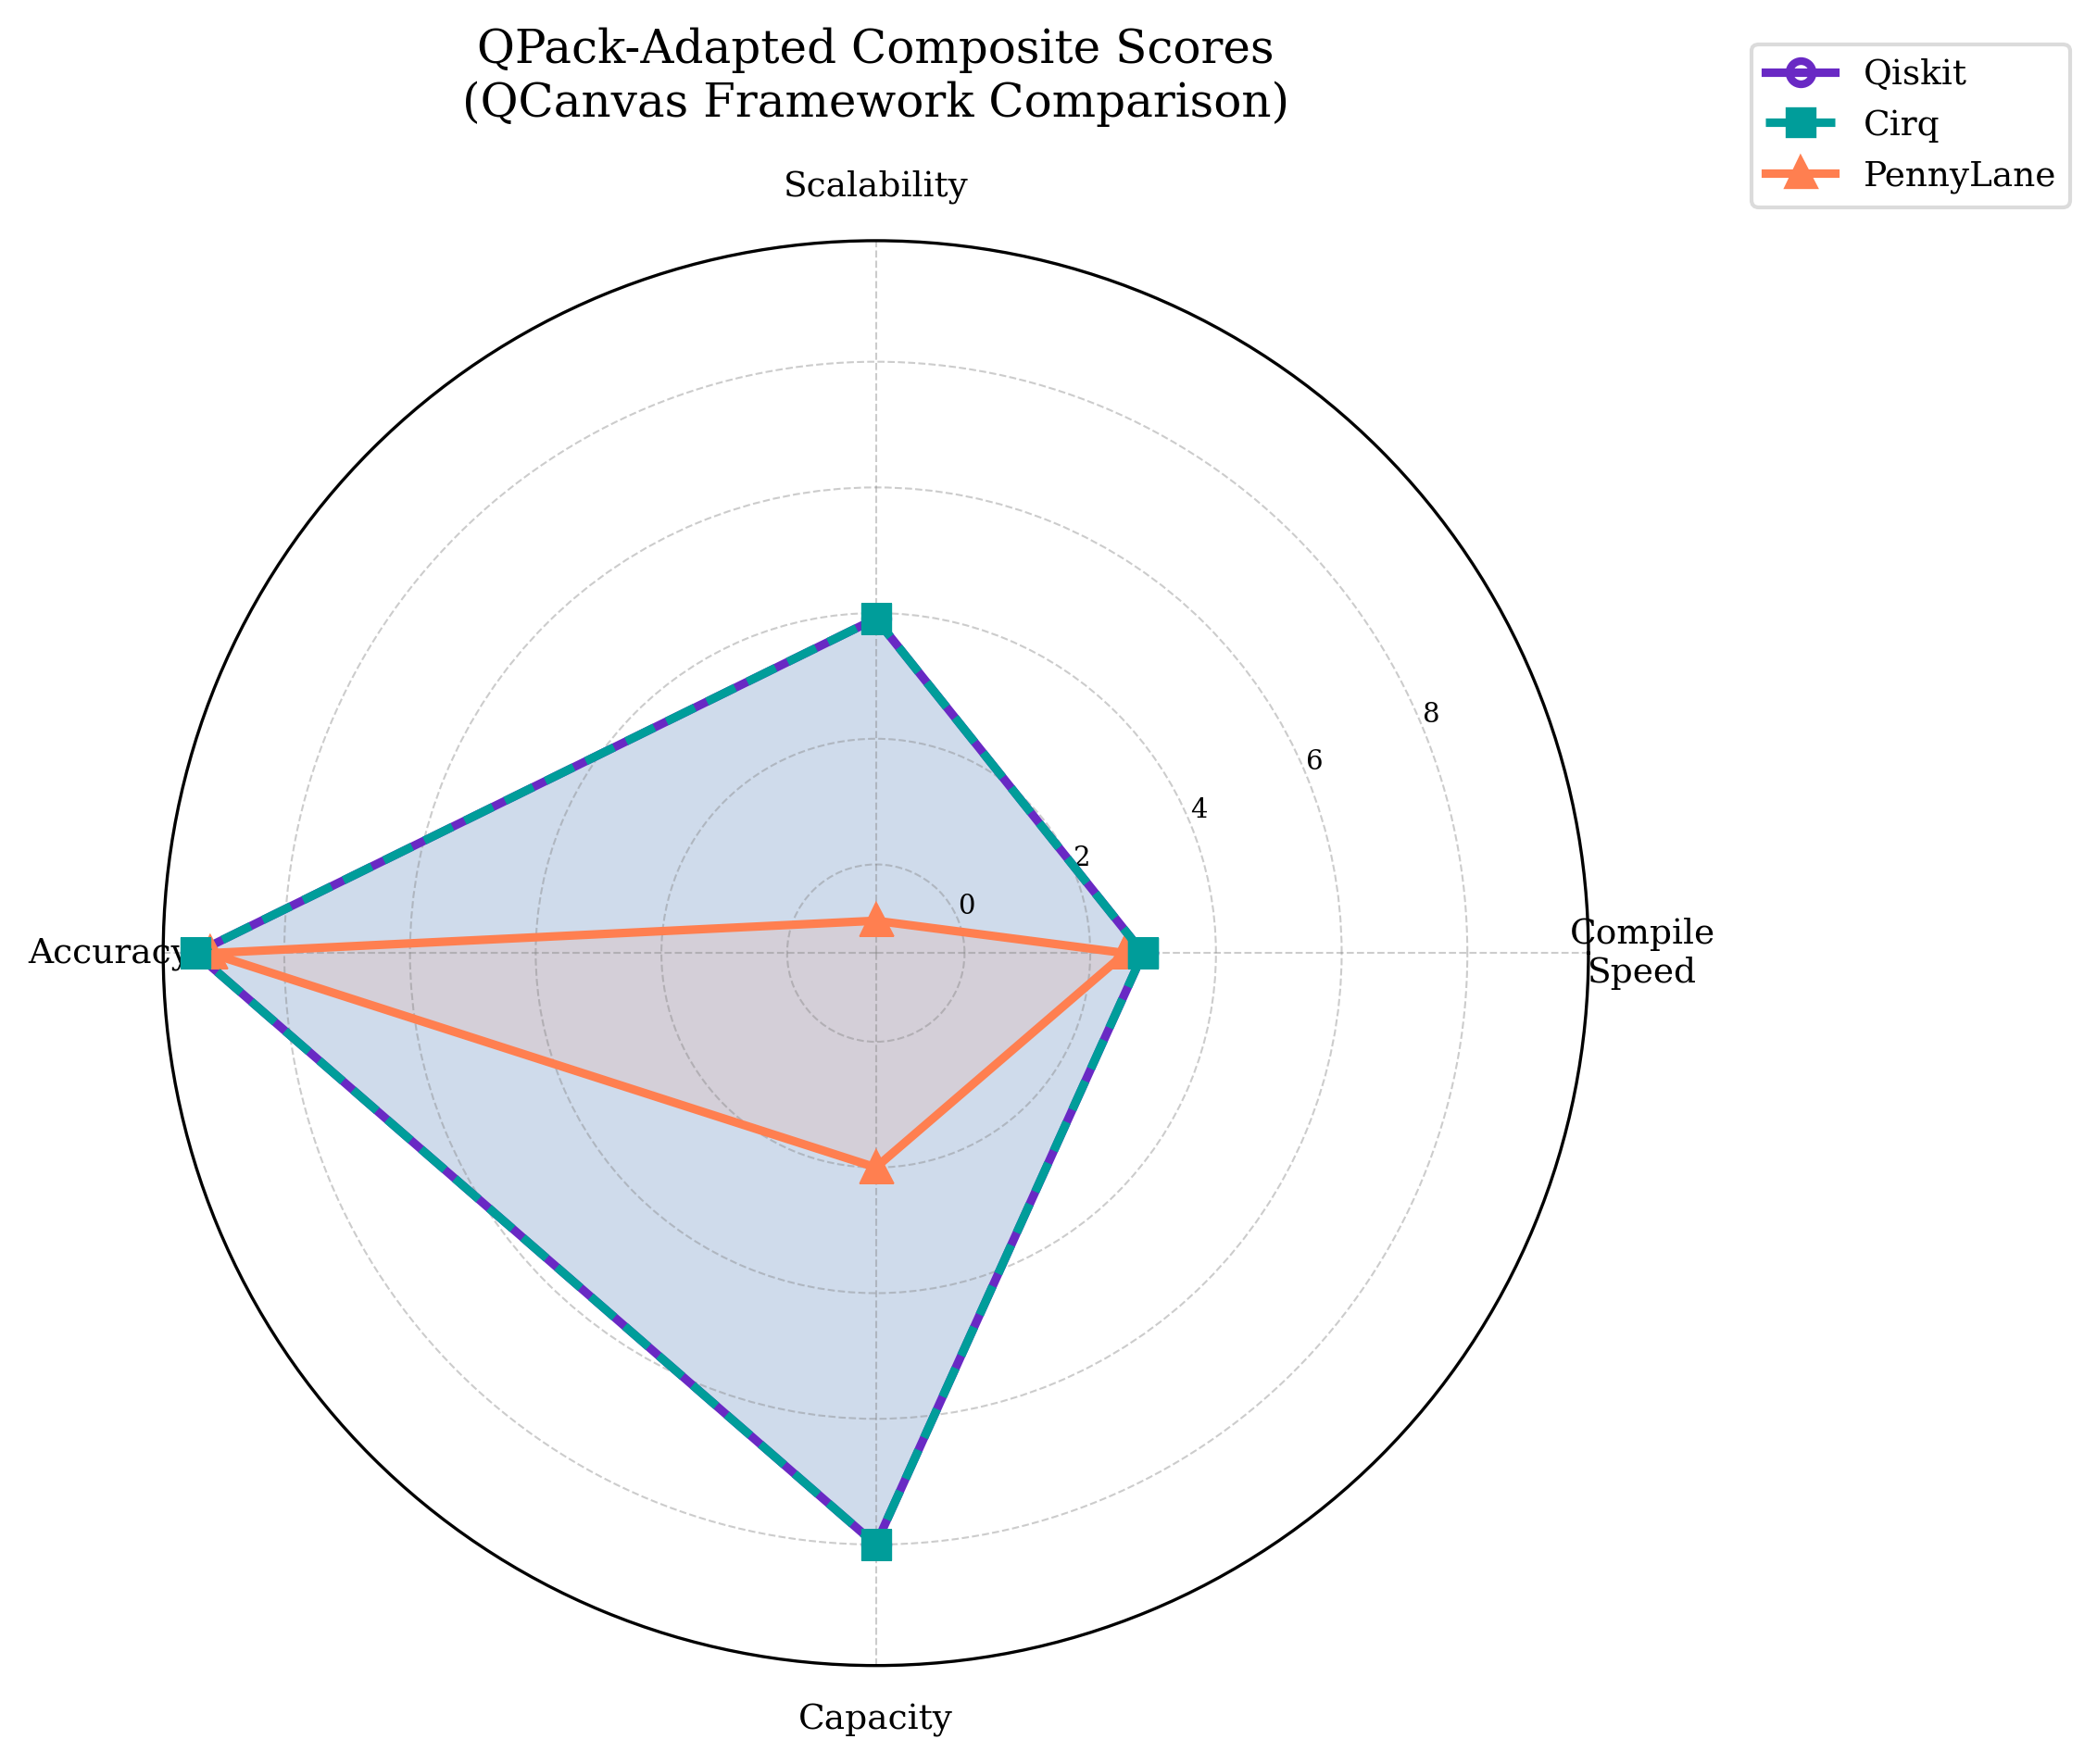
\includegraphics[width=0.80\linewidth]{fig15_qpack_radar.png}
    \caption{QPack Radar Chart --- Framework Holistic Score Comparison}
    \label{fig:qpack-radar}
\end{figure}

Qiskit and Cirq score near-identically (QPack $\approx 58.8$), substantially outperforming PennyLane (QPack $= 9.28$). PennyLane's negative scalability score ($S_\text{scale} = -0.90$) reflects its super-linear circuit growth for Grover's algorithm, which limits its applicability to larger NISQ problem sizes in default configuration.

\subsection{Performance Evaluation}

All measurements were taken on a Windows 11 host, Intel Core i7-12700H, 16 GB RAM, Python 3.11, with 10 repetitions per measurement and mean values reported.

\begin{itemize}
    \item \textbf{Conversion Latency:} Cirq circuits average 8--13ms; Qiskit 7--55ms; PennyLane 12--184ms depending on algorithm. All values satisfy NFR-P1 ($<$1500ms).
    \item \textbf{Simulation Throughput:} Grover's algorithm (6 qubits, 4096 shots) executes in under 800ms on the statevector backend (NFR-P2: $<$5 seconds).
    \item \textbf{Visualisation Render Time:} D3.js circuit diagram updates average sub-200ms for circuits up to 50 gates, satisfying NFR-P3.
    \item \textbf{Round-Trip Accuracy:} Converting standard gates to OpenQASM 3.0 and executing through QSim preserves measurement distributions with JSD $< 0.007$ against theoretical values.
\end{itemize}

\chapter{Conclusions and Future Work}
\label{ch:conclusion}

\section{Conclusion}

This final report has presented the complete development of QCanvas and QSim---a unified quantum circuit simulation and education platform---across four iterative sprints. From a standards-centered design document to a fully deployed, community-accessible pair of Python packages on PyPI, the project has achieved every major objective set out in its original specification.

\textbf{Sprint 1} established the foundational architecture: a FastAPI backend, a Next.js frontend with Monaco editor, and the core Qiskit/Cirq/PennyLane to OpenQASM 3.0 conversion pipeline. The system demonstrated that a single, standards-based intermediate representation could serve as the universal translator for disparate quantum frameworks.

\textbf{Sprint 2} deepened the platform with advanced language features (complex control flow, subroutines, bitwise operations), expanded PennyLane gate coverage, a secure database layer (PostgreSQL, Redis, Alembic migrations), and the hybrid CPU--QPU execution model that cleanly separates classical orchestration from QSim-powered quantum execution.

\textbf{Sprint 3} transformed QCanvas from a functional tool into an intelligent, community-driven learning ecosystem. The addition of real-time D3.js circuit visualization, the ``Quantum Explain It'' hover system, a gamification engine with 44 unique achievements and an XP progression system, and the recipe-sharing community platform collectively elevated the platform's educational value.

\textbf{Sprint 4} brought the project to its conclusion. Both the QCanvas converter SDK and the QSim simulation SDK were packaged and deployed to PyPI, making the FYP's core contributions accessible to the global quantum computing community. A rigorous cross-framework benchmarking study across 12 standard algorithms confirmed that Qiskit and Cirq produce structurally equivalent, constant-depth circuits and are statistically equivalent in output distribution (QPack $\approx 58.8$ each), while PennyLane's default transpiler exhibits super-linear growth for algorithms like Grover's (QPack $= 9.3$), limiting its scalability on NISQ devices. The benchmarking pipeline itself---built on top of QCanvas and QSim---serves as a reusable, reproducible research tool for the quantum computing community.

The work demonstrates that the NISQ ecosystem does not require researchers to choose between frameworks: by compiling all circuits to a common OpenQASM 3.0 intermediate representation and executing them on a shared simulation backend, QCanvas enables fair, apples-to-apples comparison and seamless framework interoperability. This result is validated both theoretically through the standards-compliance architecture and empirically through the JSD-based statistical equivalence study.

In summary, QCanvas successfully delivers:
\begin{itemize}
    \item A unified quantum IDE supporting Qiskit, Cirq, and PennyLane via a single OpenQASM 3.0 pipeline.
    \item A production-ready QSim quantum simulator SDK published on PyPI.
    \item An educational platform with hover explanations, gamification, and community sharing.
    \item A rigorous 12-algorithm, 3-framework benchmarking study with reproducible results.
    \item A complete software system with 304 passing tests, Docker deployment, and AWS-compatible infrastructure.
\end{itemize}

\section{Future Work}

Although the project has reached its FYP completion milestone, the modular architecture of QCanvas and QSim positions the platform for continued community-driven growth. The following directions represent the highest-value extensions for future contributors.

\subsection{Hardware Backend Integration}

The most natural next step is connecting QCanvas to real quantum hardware. The current architecture's pluggable QPU endpoint design means this can be achieved without structural changes to the core pipeline:
\begin{itemize}
    \item \textbf{IBM Quantum Network:} Integrate Qiskit's \texttt{IBMProvider} to dispatch compiled QASM jobs to real IBM QPUs, using the same \texttt{/simulate} API endpoint.
    \item \textbf{AWS Braket:} Leverage Amazon Braket's OpenQASM support to run circuits on IonQ, Rigetti, and OQC hardware without changing the compilation pipeline.
    \item \textbf{Google Quantum Computing Service:} Target Sycamore processors via Cirq's GCS backend.
\end{itemize}

\subsection{Noise-Aware Simulation and Error Mitigation}

\begin{itemize}
    \item \textbf{Noise Model Integration:} Extend QSim to support realistic noise models (depolarizing, amplitude damping, phase damping) for hardware-accurate simulation.
    \item \textbf{Error Mitigation Techniques:} Implement zero-noise extrapolation and measurement error mitigation within the QSim execution pipeline.
    \item \textbf{Noise-Aware Compilation:} Select gate decompositions and circuit layouts that minimize expected error rates based on a user-specified noise model.
\end{itemize}

\subsection{Expanded Framework Support}

The plug-in architecture of the converter layer enables straightforward addition of new quantum frameworks:
\begin{itemize}
    \item \textbf{Q\# (Microsoft):} Convert Microsoft Q\# programs to OpenQASM 3.0 via Q\#'s Python interop layer.
    \item \textbf{PyQuil (Rigetti):} Support Quil-based circuits from Rigetti's Forest SDK.
    \item \textbf{Amazon Braket SDK:} Parse Braket circuit objects and compile them to OpenQASM 3.0.
    \item \textbf{TKET (Pytket):} Leverage pytket's built-in OpenQASM export for t$|$ket$\rangle$ circuit support \cite{sivarajah2020tket}.
\end{itemize}

\subsection{Advanced Visualization and Analytics}

\begin{itemize}
    \item \textbf{Bloch Sphere Animation:} Animated Bloch sphere visualization showing qubit state evolution gate by gate.
    \item \textbf{Entanglement Graph:} Graph-based representation of qubit entanglement relationships throughout circuit execution.
    \item \textbf{Probability Heatmaps:} Visual representation of full measurement probability distributions across all possible bitstring outcomes.
    \item \textbf{AI-Powered Optimization Suggestions:} Circuit simplification recommendations powered by LLM-based gate analysis.
\end{itemize}

\subsection{Community and Research Collaboration}

\begin{itemize}
    \item \textbf{GitHub-Style Circuit Repository:} Git-like versioning for circuits, forking, merging, and community review threads.
    \item \textbf{Research Reproducibility Tools:} Circuit versioning with full execution environment snapshots; automated experiment documentation and LaTeX export.
    \item \textbf{Adaptive Learning System:} Machine learning-based personalization that adjusts content difficulty and example recommendations based on individual learning history.
    \item \textbf{Public REST API with OAuth 2.0:} Tiered rate-limited API access for external applications and CI/CD quantum testing pipelines.
\end{itemize}

\subsection{Production Infrastructure Hardening}

\begin{itemize}
    \item \textbf{Kubernetes Deployment:} Migration from Docker Compose to a Kubernetes cluster with horizontal pod autoscaling.
    \item \textbf{gRPC Communication:} Replace REST-based QCanvas--QSim communication with optimized gRPC endpoints for lower-latency execution.
    \item \textbf{Distributed Tracing:} End-to-end request tracing across frontend, backend, and QSim services using OpenTelemetry.
    \item \textbf{Multi-Factor Authentication:} TOTP-based MFA support to strengthen the authentication system.
\end{itemize}


\appendix
\chapter*{Appendix}
\addcontentsline{toc}{chapter}{Appendix}

\section*{A. PyPI Package Listings}

Both SDK packages are publicly available on the Python Package Index:
\begin{itemize}
    \item \textbf{QSim SDK:} \texttt{pip install qsim-sdk} \\
    Provides \texttt{StatevectorBackend}, \texttt{DensityMatrixBackend}, and \texttt{StabilizerBackend} classes for executing OpenQASM 3.0 circuits programmatically.
    \item \textbf{QCanvas SDK:} \texttt{pip install qcanvas-sdk} \\
    Provides the \texttt{QCanvas\-Converter} class for converting Qiskit, Cirq, and PennyLane circuits to OpenQASM 3.0 source and AST.
\end{itemize}

\section*{B. Benchmark Compilation Times -- Full Summary}

The table below shows mean compilation latency (ms) and standard deviation across all benchmark algorithms at their maximum tested qubit count. All values are within the NFR-P1 target of 1500ms.

\begin{table}[H]
\centering
\caption{Compilation Latency Summary -- All Algorithms at Maximum Qubit Count}
\label{tab:compile-full}
\resizebox{\textwidth}{!}{%
\begin{tabular}{|l|l|r|r|r|}
\hline
\textbf{Algorithm} & \textbf{Max Qubits} & \textbf{Qiskit (ms)} & \textbf{Cirq (ms)} & \textbf{PennyLane (ms)} \\ \hline
Bell State & 2 & 18.6 $\pm$ 0.4 & 8.3 $\pm$ 0.5 & 12.2 $\pm$ 0.3 \\ \hline
GHZ State & 8 & 21.9 $\pm$ 0.9 & 10.7 $\pm$ 0.4 & 38.0 $\pm$ 0.9 \\ \hline
Quantum Teleportation & 3 & 38.7 $\pm$ 0.9 & 15.6 $\pm$ 0.6 & 24.7 $\pm$ 0.6 \\ \hline
Deutsch--Jozsa & 8 & 7.0 $\pm$ 0.3 & 12.1 $\pm$ 1.3 & 106.3 $\pm$ 3.4 \\ \hline
Bernstein--Vazirani & 8 & 17.5 $\pm$ 0.6 & 13.0 $\pm$ 0.5 & 98.9 $\pm$ 2.5 \\ \hline
Grover's Algorithm & 6 & 9.6 $\pm$ 0.5 & 32.5 $\pm$ 1.9 & 184.2 $\pm$ 6.5 \\ \hline
QRNG & 8 & 12.8 $\pm$ 0.4 & 10.3 $\pm$ 0.2 & 37.0 $\pm$ 0.5 \\ \hline
VQE & 6 & 32.9 $\pm$ 3.9 & 13.8 $\pm$ 1.0 & 55.2 $\pm$ 2.9 \\ \hline
QAOA & 6 & 55.0 $\pm$ 3.2 & 19.1 $\pm$ 2.6 & 73.7 $\pm$ 7.2 \\ \hline
QML XOR Classifier & 4 & 47.9 $\pm$ 4.8 & 21.0 $\pm$ 1.6 & 73.9 $\pm$ 5.9 \\ \hline
Bit-Flip Code & 3 & 55.5 $\pm$ 27.0 & 14.0 $\pm$ 1.4 & 35.0 $\pm$ 4.1 \\ \hline
Phase-Flip Code & 3 & 64.8 $\pm$ 11.4 & 22.4 $\pm$ 5.3 & 54.7 $\pm$ 5.1 \\ \hline
\end{tabular}%
}
\end{table}

\section*{C. Quantum Volume Estimates -- Bell State Baseline}

Effective Quantum Volume ($\log_2 = 11$, QV = 2048) is identical across all three frameworks under ideal (noise-free) simulation, confirming that QSim provides a level execution substrate. Divergence in structural metrics (gate count, circuit depth) reflects compiler strategy differences only.


\addcontentsline{toc}{chapter}{References}
\bibliographystyle{plain}
\bibliography{references}

\end{document}
